\documentclass{book}

\usepackage{talmey}

\begin{document}
\begin{titlepage}
    \begin{center}
        \fontsize{50}{50}\selectfont \textbf{\so{IDO}}
        \vfill
        \Huge Exhaustive Text Book of the \\ International Language \\ of the Delegation \\
        \vspace{0.25cm}
        \normalsize \emph{and} \\ 
        \vspace{0.1cm}
        \Large Fundamentals of an \\ Artificial International Language
        \vfill
        \emph{By} \\
        \vspace{0.25cm}
        DR. MAX TALMEY \\ 
        \vspace{0.25cm}
        \emph{Author of Practical and Theoretical Esperanto, \\ Defects of Esperanto, etc.}
        \vfill
        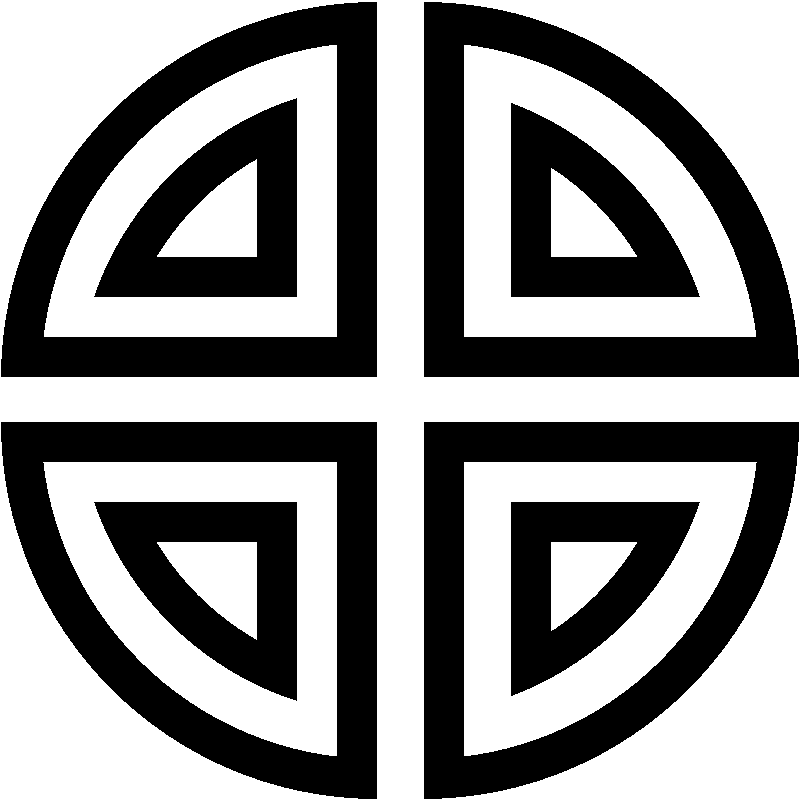
\includegraphics[height = 1.125cm, width = 1.125cm]{symbol.png}
        \vfill
        \textsc{Ido Press, New York} \\
        \rule{0.2\textwidth}{.4pt} \\
        1919
    \end{center}
\end{titlepage}

\tableofcontents

The citations from the magazine Progreso are designated by a Roman number indicating the volume of the magazine, followed by an Arabic number for the page in that volume, both in parentheses. A decision of the Ido academy is designated by dec.

\section*{PREFACE.}
\addcontentsline{toc}{section}{Preface: Essentials of the history of the international language in general; of Volapük and Esperanto; causes of their failure; origin, development, and definition of Ido; aim of this text book}
\lettrine{T}{o} enter upon the study of an international language in an intelligent manner some knowledge of the history of the attempts to create an international language is indispensable. A few of the most important historical data will therefore be briefly presented here. For a more thorough information reference is made to the excellent work on the subject by Dr.~L.~Couturat and Dr.~L.~Leau: Histoire de la Langue Universelle, a volume of nearly 600 pages treating historically and critically all artificial languages devised until about 1903. 

The history of artificial international languages dates back nearly 300 years. During this period about 250 idioms have been constructed. They reveal a gradual evolution from crude linguistic devices, hardly deserving the name language, in the beginning, to more or less perfect languages in recent times, the later systems, as a rule, surpassing the earlier ones in quality. 

From the beginning of this period to our times the problem of an artificial international language has occupied, to a greater or lesser degree, the minds of some of the greatest thinkers and scholars. Among them are to be mentioned Bacon, Descartes, Leibnitz, Voltaire, Alex.~v.~Humboldt, J.~v.~Grimm, A.~M.~Lamartine, Victor Hugo, Ernest Naville, W.~Förster, H.~Schuchardt, W.~Ostwald, Otto Jespersen, etc. 

Of all artificial languages Volapük and Esperanto have gained the widest publicity. It is impossible to establish which of the two had the larger number of adherents, for the reports in this respect are entirely unreliable. 

Volapük was devised by the German priest Schleyer of Konstanz, Baden, and published in 1880. It spread rapidly in all civilized countries and flourished until 1889. Then it began to lose ground and declined as rapidly as it had risen and was soon forgotten. Intrinsic defects of the language, which became apparent at the congress of Volapükists in Paris in 1889, and failure of its advocates to come to an understanding as to the way to amend them furnished the causes for its downfall. 

Esperanto was devised by the Russian physician Dr.~L.~Zamenhof of Warsaw while Volapük was still at its height and published in 1887. Its progress was very slow until the Frenchman Marquis L. de Beaufront, an eminent philologist, began to take interest in it about 1890. He became the second father of Esperanto by creating a real language out of the crude sketch of its inventor, and to him more than to anybody else is due the fact that Esperanto became known in every civilized country gaining everywhere great numbers of adherents many of whom still swear faithful allegiance to it. 

Esperanto has attained a high degree of perfection and in many respects it excels all artificial languages preceding it and those which were devised as a result of the disintegration of Volapük. Because of its good features competent students of the problem of an international language praised and advocated it. They were well aware that it contained also substantial defects and pointed them out. But they recognized that these imperfections could be remedied and hoped that the necessary reforms would be introduced soon enough to prevent the language from deteriorating through its defects to such an extent as to be beyond correction. 

The proper opportunity for starting the reforms of Esperanto came in 1907. In October of this year the Committee of the International Delegation for the Adoption of an International Auxiliary Language convened in Paris for the purpose which had brought the Delegation into existence at the Paris exposition in 1900. This purpose was to procure to the civilized nations an auxiliary international language either by endorsing one of the existing artificial languages or by constructing a new one if none of the existing ones were found adequate. The Committee composed of scholars of international reputation examined many artificial languages and rejected them all, including Esperanto in its original form. It adopted, however, Esperanto in principle under reserve of certain modifications to be introduced by the Permanent Commission of the Delegation in the sense defined by the report of the secretaries of the Committee and by the project of Ido which had also been presented for examination. Besides, the Committee recommended an understanding with the Linguistic Committee for Esperanto. When subsequently this understanding was sought, the majority of the Esperanto Committee, or at least that number of its members which was given out as its majority, refused absolutely to recognize the necessity of reforming Esperanto, and all negotiations in this respect had to be broken off. The Permanent Commission of the Delegation thereupon went its own way beginning a systematic further development and perfection of the project of Ido. 

The Esperanto Committee also went its own way. But its failure to agree with the Permanent Commission of the Delegation caused Esperanto to lose ground everywhere. The deterioration of the language which had already commenced before continued now unchecked and is still continuing so that the language has become so overcharged with absurdities as to be entirely unfit for the role of an international language. 

It is evident that the history of Volapuk is repeating itself in Esperanto, though at a slower pace owing to the relative superiority of the latter over the former. The primary cause for the retrogression of Esperanto lies in substantial philological defects which have called forth sharp criticism from the most competent sources. The foremost of these linguistic defects is a faulty system of derivation or rather lack of a proper system of derivation. For while other imperfections, as peculiar letters not contained in any other language, cacophony, too much inflection, can not render the language more imperfect than it was in its original form, faulty derivation increases the faults in leading to absurd word formations which by-and-by become an integral part of the language. This defect of Esperanto has been most clearly expounded by Dr.~L.~Couturat in his lucid monograph: Etude sur la Dérivation en Esperanto. 

These linguistic defects, however, could and would have been remedied but for the chief cause of Esperanto's decline. It consists in the most influential leaders of Esperanto having endeavored and succeeded to make Esperanto the medium of a sort of new religion called Esperantism or Homaranism and proclaiming that a common language of the nations in general and of Esperanto in particular would bring about universal brotherhood of men. As the medium of a religion Esperanto became inviolable, was not to be subjected to criticism, much less to change or reform. The fallacy of this new religion has been pointed out by the author (Progreso, I, p. 83). To still further strengthen the inviolability of the medium of the new religion the ridiculous assertion was put forward that Esperanto was the living language of a living people---vivanta lingvo de vi vanta popolo. Here every argument had to stop, for a living language must indeed not be touched. 

Entirely different was the policy of the Permanent Commission of the Delegation which undertook to develop the project of Ido. It founded in its behalf an official organ, Progreso, and an academy and invited criticism from all sides to be either published in this magazine or presented directly to the academy which was then to introduce the change in the language necessary to correct the imperfect feature criticised. 

Ido is the pseudonym under which the foremost Esperantist Marquis L. de Beaufort presented to the Committee of the Delegation for examination several documents, a complete grammar, Grammaire Complète, an elementary grammar, and a short dictionary. They completely outlined a new language devoid of the defects of Esperanto while preserving its good features. It is actually this language that the Committee adopted after rejecting all others examined. But the decision to this effect was evidently drafted with the view to gain the adherence to the new language of the great number of those who favored original Esperanto. The decision reads: “Le Comité a décidé d’adopter en principe l’Esperanto \ldots sous la resérve de certaines modifications \ldots à exécuter \ldots dans le sens défini \ldots par le projet de Ido.” Esperanto, accordingly, was to be modified in conformity with this project, not inversely. Any other modern artificial language modified in this sense would have given the same result. Only a few more modifications would have been required. For the modern artificial languages resemble each other a good deal. The view, therefore, that the new language represents simplified Esperanto, has to be taken cum grano salis. At the present day after further deterioration of Esperanto on one side, and considerable further improvement of the new language through its academy on the other side, the difference between the two is very great, so that that view cannot at all be maintained any longer. 

During the negotiations aiming at an understanding with the Esperanto Committee and for quite some time after they had been broken off, the new language was officially known under the name International Language of the Delegation. For about two years the name Ilo, constructed from the letters I and L of the term International Language, was favored by many and frequently used by writers. Several other names were proposed. But finally the pseudonym Ido of Mr. de Beaufront was adopted by the Committee of the Union of Idists (II, 288) and found general acceptance as the name of the new language. 

Already from the beginning Ido was far superior to any artificial language ever devised. Through the painstaking strictly scientific work of the academy during the past seven years and through its liberal policy of inviting and considering every criticism, important changes and additions, notably in the vocabulary, have been made whereby Ido has attained a still higher degree of perfection. Recently the academy has decreed a period of stability of ten years during which no further changes are to be made. It may safely be stated that only very few will be required after the lapse of this period. The construction of Ido is thus completed and authors of text books are now enabled to offer to students work of lasting value.

Ido is therefore to be defined as the language laid down in the “Grammaire Complète par Ido” and modified and amplified by the decisions of the Ido academy. This text book conforms strictly to this definition, setting forth only the rules, and all the rules, sanctioned by these two authorities. The official organ Progreso has been freely consulted and numerous references to it have been given for explaining and illustrating grammatical rules and forms of good style. 

The object of this work is not only to enable the average scholar to acquire a good working knowledge of the language, but also to acquaint the accomplished student with the principles to be observed in the construction of an artificial language, to point out to him niceties of grammar and stylistic that are requisite to proficiency in the international language, and to help him over many linguistic difficulties. All grammars of Esperanto and Ido are incomplete in this respect. The serious student of Ido had therefore to resort frequently to the official magazine for enlightenment as shown by the numerous linguistic questions (“linguala questioni”) treated extensively in almost every number of the seven volumes of Progreso and representing its best feature. To supply this want has been a most important aim of this work. \begin{flushright}New York, January 1914.\end{flushright}

The first draft of this book was read and approved in the spring of 1914 by the foremost authority on the problem of an international language, Dr.~L.~Couturat. He characterized the book as very carefully and conscientiously composed (“la libro esas tre sorgoze e konciencoze kompozita”). This warranted the belief that the work did not remain far away from its aim. Its publication was to take place in the fall of 1914, but was prevented by the outbreak of the world war. The manuscript was locked away to be taken up again at a time more propitious for a work intended to promote international intercourse. When this time approached not long ago, the work was resumed. A good deal of material was added to bring the book still nearer its aim. Most of the material of importance to the accomplished student and teacher, which in the first draft was scattered here and there in the form of notes, was gathered into a separate part, the fourth one. The average scholar needs to pay but little attention to this part. 
\RaggedLeft New York, June 1919. \justifying


\section*{SUMMARY OF THE IDO GRAMMAR.}
\addcontentsline{toc}{section}{Summary of the Ido Grammar}
To understand any Ido text without previous study of the language all that is needed is a perusal of the summary, given below, which in a little more than two pages contains all essentials of the Ido grammar. One knowing Latin or one Roman language will not even have to resort to an Ido dictionary. Before commencing the actual study of the language he is thus enabled to estimate its merits by reading a few Ido texts. For this reason the summary of the Ido grammar and a few such texts have been put at the beginning of this text book and not at its end, where they would belong more properly. Those who know no other language besides English will do better to read first parts one to three, then the summary, and finally the Ido texts. 

Pronunciation.—The vowels of Ido have the continental pronunciation (see “continental” in Standard Dictionary). Of two succeeding vowels, as \textbf{au}, \textbf{eu}, \textbf{ia}, \textbf{io}, each one is to be pronounced. \textbf{C} is pronounced like ts in wits and \textbf{j} like the French j. The accent rests on the last syllable but one, and in words ending in \textbf{-ar}, \textbf{-ir}, \textbf{-or} on the last syllable. \textbf{I} and \textbf{u} preceding immediately the end vowel of a word that contains more than two vowels cannot have the accent. The latter must then be put on the vowel which precedes the \textbf{i} or the \textbf{u}. 

\begin{enumerate}
    \item The definite article is \textbf{la} for singular and plural, and \textbf{le} for the plural when no other word indicates the latter. The article \textbf{lo} before an adjective denotes the neuter of it: \textbf{lo bela}, the beautiful. A noun alone includes the indefinite article.
    \item Every word of two or more syllables that ends in \textbf{-o} is a noun; in \textbf{-a} an adjective; in \textbf{-e} an adverb or preposition; in \textbf{-u} a pronoun; in \textbf{-i} the plural of a noun or pronoun; in \textbf{-on}, \textbf{-an}, \textbf{-un}, \textbf{-in} the accusative form of a noun, adjective, pronoun, or of a plural, respectively; in \textbf{-ar}, \textbf{-ir}, \textbf{-or} the infinitive of the present, past, or future, respectively; in \textbf{-as}, \textbf{-is}, \textbf{-os} a verb in the present, past, or future, respectively; in \textbf{-ez}, \textbf{-us} a verb in the imperative or conditional, respectively. The active participle as adjective ends in \textbf{-anta}, \textbf{-inta}, \textbf{-onta} and the passive participle; in \textbf{-ata}, \textbf{-ita}, \textbf{-ota} in the present, past, and future, respectively. As noun or adverb the participle ends in \textbf{-o} or \textbf{-e}, respectively.
    \item The comparative of the adjective and adverb is formed by \textbf{plu}, more, and \textbf{min}, less; the superlative by \textbf{maxim}, most, and \textbf{minim}, least.
    \item There is no distinction of number and person with verbs. 
    \item The passive voice is formed with the passive participle and the verb \textbf{esar}, to be; the compound tenses are formed with \textbf{esar} and the participle of the past. The passive voice may also be formed with the suffix \textbf{-es}, and the compound tenses with the suffix \textbf{-ab}. These suffixes are inserted between the verbal root and the ending. \textbf{Me esas amata} or \textbf{me amesas}, I am loved. \textbf{Me esos aminta} or \textbf{me amabos}, I shall have loved. 
    \item The personal pronouns are: \textbf{me}, I; \textbf{tu}, you, thou; \textbf{il}, he; \textbf{el}, she; \textbf{ol}, it; \textbf{lu}, he, she, it; \textbf{lo}, it (referring to a fact); \textbf{ni}, we; \textbf{vi}, you (several persons); \textbf{vu}, you (one person); \textbf{li}, they; \textbf{ili}, they (masculine); \textbf{eli}, they (feminine); \textbf{oli}, they (neuter); \textbf{on}, one, we, they (indefinite); \textbf{su}, one’s self (reflexive). The possessive pronouns formed from the personal pronouns are: \textbf{mea}, my, mine; \textbf{tua}, your, yours; \textbf{lua}, his, hers, its, etc. 
    \item The demonstrative, relative, and interrogative pronouns are: \textbf{ca}, \textbf{ica}, \textbf{ilea}, \textbf{elca}, \textbf{olca}, this; \textbf{ci}, \textbf{ici}, etc., these; \textbf{ta}, \textbf{ita}, \textbf{ilta}, \textbf{elta}, \textbf{olta}, that; \textbf{ti}, \textbf{iti}, etc., those; \textbf{qua}, \textbf{ilqua}, etc., who, which, that; plural: \textbf{qui}, who, which, that; neuter: \textbf{co}, this; \textbf{to}, that; \textbf{quo}, what. 
    \item The determinatives are: \textbf{altra}, another; \textbf{ipsa}, self; \textbf{irga}, any whatever; \textbf{kelka}, some; \textbf{multa}, much; \textbf{nula}, none; \textbf{omna}, all, every; \textbf{plura}, several; \textbf{poka}, little; \textbf{quala}, what kind of; \textbf{quanta}, how much; \textbf{sama}, same; \textbf{singla}, every single; \textbf{tala}, such; \textbf{tanta}, so much; \textbf{ula}, some, a certain. As pronouns these words end in singular in \textbf{-u} and in plural in \textbf{-i}. 
    \item The numbers are: \textbf{zero}, 0; \textbf{un}, 1; \textbf{du}, 2; \textbf{tri}, 3; \textbf{quar}, 4; \textbf{kin}, 5; \textbf{sis}, 6; \textbf{sep}, 7; \textbf{ok}, 8; \textbf{non}, 9; \textbf{dek}, 10; \textbf{dek e un}, 11; \textbf{dek e du}, 12, etc.; \textbf{duadek}, 20; \textbf{triadek}, 30; \textbf{quaradek}, 40, etc.; \textbf{kinadek e sis}, 56; \textbf{sisadek e sep}, 67, etc.; \textbf{cent}, 100; \textbf{cent e un}, 101; \textbf{cent e nonadek e tri}, 193; \textbf{okacent}, 800; \textbf{mil}, 1000; \textbf{sepamil}, 7000; \textbf{milion} (accent on the o), million.
    
    The ordinal and fractional numbers are formed by the endings \textbf{-esma} and \textbf{-imo} respectively. When these numbers are nouns they end in \textbf{-esmo} and \textbf{-imo}. 
    \item The prepositions have no characteristic endings: \textbf{a} (\textbf{ad}), to; \textbf{de}, from; \textbf{di}, of; \textbf{da}, by; \textbf{ek}, from; \textbf{lor}, at the time of; \textbf{kun}, with; \textbf{pri}, about; \textbf{sen}, without; \textbf{ye}, at, in, on, with; etc. 
    \item Coordinate conjunctions are: \textbf{do}, then, therefore; \textbf{e} (\textbf{ed}), and; \textbf{ka} (\textbf{kad}) introduces a direct question; \textbf{ma}, but; \textbf{o} (\textbf{od}), or; \textbf{nam}, for; \textbf{ya}, certainly, indeed; etc.
    
    Subordinate conjunctions are: \textbf{ka} (\textbf{kad}), whether, if; \textbf{kande}, when; \textbf{ke}, that; etc. 
    \item Word Formation. New words are formed by prefixes and suffixes. The former precede the word, the latter are inserted between the root and the grammatical endings. 
\end{enumerate}
\begin{center}The prefixes are:\end{center}
\textbf{anti-}, against: \textbf{antipolo}, antipole;  \\
\textbf{arki-}, arch: \textbf{arkianjelo}, archangel; \\
\textbf{bo-}, relationship by marriage: \textbf{bopatro}, parent-in-law; \\
\textbf{des-}, contrary: \textbf{deshonoro}, dishonor; \\ 
\textbf{dis-}, dispersion: \textbf{disdonar}, to distribute; \\ 
\textbf{ex-}, former office: \textbf{exprezidanto}, ex-president; \\ 
\textbf{gala-}, gala: \textbf{galadio}, galaday; \\ 
\textbf{ge-}, persons of both sexes: \textbf{gepatri}, parents; \\ 
\textbf{mi-}, half: \textbf{mifratino}, half sister; \\ 
\textbf{mis-}, wrong action: \textbf{misguidar}, to misguide; \\ 
\textbf{ne-}, negation: \textbf{nevidebla}, invisible; \\ 
\textbf{par-}, thoroughness: \textbf{parlernar}, to learn thoroughly;
\textbf{para-}, protection against: \textbf{parapluvo}, umbrella; \\ 
\textbf{pre-}, pre-: \textbf{prematura}, premature; \\ 
\textbf{retro-}, back: \textbf{retrosendar}, to send back; \\ 
\textbf{ri-}, repetition: \textbf{rividar}, to see again; \\ 
\textbf{sen-}, less: \textbf{senmova}, motionless; \\ 
\textbf{stifa-}, step-: \textbf{stifafilio}, stepchild. 

\begin{center}The suffixes are:\end{center}
\textbf{-ach}, pejorative: \textbf{medikacho}, quack; \\ 
\textbf{-ad}, duration: \textbf{pafado}, fusillade; \\ 
\textbf{-ag}, acting with: \textbf{krucagar}, to crucify; \\ 
\textbf{-aj}, something, consisting of: \textbf{molajo}, something soft; \textbf{lignajo}, woodwork; \\ 
\textbf{-al}, relating to: \textbf{nacionala}, national; \\ 
\textbf{-an}, member of: \textbf{senatano}, senator; \\ 
\textbf{-ar}, collection of: \textbf{vortaro}, vocabulary; \\ 
\textbf{-ari}, passive participator: \textbf{pagario}, payee; \\ 
\textbf{-atr}, of the nature of: \textbf{kupratra}, copperlike; \\ 
\textbf{-e}, of the color of: \textbf{rozea}, rose colored; \\ 
\textbf{-ebl}, capable of being: \textbf{videbla}, visible; \\ 
\textbf{-ed}, certain quantity: \textbf{glasedo}, a glassful; \\ 
\textbf{-eg}, augmentative: \textbf{grandega}, immense; \\ 
\textbf{-em}, inclined to: \textbf{babilema}, talkative; \\ 
\textbf{-end}, to be done; \textbf{adjuntenda}, to be added; \\ 
\textbf{-er}, -er: \textbf{fumero}, smoker; \\ 
\textbf{-eri}, establishment: \textbf{kafeerio}, cafe; \\ 
\textbf{-es}, abstract quality, passive of a verb: \textbf{saneso}, health; \textbf{amesar}, to be loved; \\ 
\textbf{-esk}, to become, to begin: \textbf{paleskar}, to become pale; \textbf{dormeskar}, to fall asleep; \\ 
\textbf{-esm}, ordinal number; \textbf{quaresma}, fourth; \\ 
\textbf{-estr}, head of: \textbf{navestro}, captain; \\ 
\textbf{-et}, diminutive: \textbf{ridetar}, to smile; \\ 
\textbf{-ey}, place destined for: \textbf{tombeyo}, cemetery; \\ 
\textbf{-foy}, time: \textbf{trifoya}, of three times; \\ 
\textbf{-i}, domain: \textbf{episkopio}, diocese; \\ 
\textbf{-id}, offspring: \textbf{Napoleonido}, offspring of N.; \\ 
\textbf{-ier}, characterized by, bearer of: \textbf{kurasiero}, cuirassier; \textbf{pomiero}, apple tree; \\ 
\textbf{-if}, to produce; \textbf{pomifar}, to bear apples; \\ 
\textbf{-ig}, to make, to render: \textbf{purigar}, to purify; \textbf{dormigar}, to put asleep;
\textbf{-ik}, sick with: \textbf{diabetika}, sick with diabetes; \\ 
\textbf{-il}, instrument: \textbf{tranchilo}, cutting instrument; \\ 
\textbf{-im}, fraction: \textbf{duimo}, half; \textbf{quarimo}, quarter; \\ 
\textbf{-in}, female sex: \textbf{spozino}, wife; \textbf{bovino}, cow; \\ 
\textbf{-ind}, worthy: \textbf{imitinda}, worthy of imitation; \\ 
\textbf{-ism}, system, doctrine: \textbf{socialismo}, socialism; \\ 
\textbf{-ist}, professional occupation: \textbf{artisto}, artist; \\ 
\textbf{-iv}, capable of doing: \textbf{instruktiva}, instructive; \\ 
\textbf{-iz}, to provide with: \textbf{armizar}, to arm; \\ 
\textbf{-op}, distributive number: \textbf{triope}, by three; \\ 
\textbf{-opl}, multiplicative number: \textbf{dekopla}, tenfold; \\ 
\textbf{-oz}, containing: \textbf{sabloza}, sandy; \\ 
\textbf{-ul}, male sex: \textbf{spozulo}, husband; \textbf{bovulo}, ox; \\ 
\textbf{-um}, indefinite or general suffix: \textbf{krucumar}, to cross; \textbf{kolumo}, collar; \\ 
\textbf{-ur}, result of an action: \textbf{pikturo}, painting; \\ 
\textbf{-uy}, recipient: \textbf{sukruyo}, sugar box. 

Keeping in mind the preceding 11 short paragraphs of grammar and considering to some extent the 12th one about word derivation, the intelligent student will have no difficulty in understanding the following Ido texts. That Ido is intelligible almost at first sight is due to the internationality of its vocabulary which is built strictly a posteriori. This may be seen from the same Esperanto texts. They are much less comprehensible mainly because the Esperanto vocabulary is far less international and to a great extent arbitrarily selected. 

Grammatically Esperanto differs from Ido by the plural endings \textbf{-oj}, \textbf{-aj}, \textbf{-uj} of noun, adjective, and pronoun respectively; by the endings \textbf{-i} and \textbf{-u} of the infinitive and imperative respectively; by the obligatory application of the accusative (\textbf{-on}, \textbf{-ojn}, \textbf{-ajn}, \textbf{-ujn}) for the direct object and otherwise; finally by the variability of the adjective in case and number. 

The comparison of the texts will also bring out clearly the euphony of Ido and the extreme cacophony of Esperanto which is due to the abundance of the sibilants and the excessive repetition of the combinations \textbf{oj}, \textbf{aj}, \textbf{uj}, \textbf{ojn}, \textbf{ajn}, \textbf{ujn}. (The Esperanto j is pronounced like the English y in young.) 

It will be noticed that the unconnected sentences given below are not at all far fetched like the English catch: Chichester church stands in Chichester church yard. On the contrary, they are ordinary, every-day phrases, yet they sound in Esperanto like that catch in English.


\section*{COMPARATIVE TEXTS OF ESPERANTO AND IDO.}
\addcontentsline{toc}{section}{Comparative Texts of Esperanto and Ido}
I.
\begin{parcolumns}{2}
    \colchunk{%
        \begin{otherlanguage}{esperanto}
        \begin{center}Esperanto\end{center}
        Ĝu ŝi scias ĉion?\footnotemark[1] \\
        Ĝu ŝi ciam rugigas pri ĉio? \\
        Ĝu ŝia voĉo placas al vi? \\
        Ĝu sia fianĉo sercis sin? \\
        Car ŝi ne scias, ĉu ŝia ĉapelo estas tie-ĉi aŭ ĉe ŝia ĉambro, sercu ĝin ĉie.  \\
        Ŝi ĉiam ĉarmas ĉiujn per sia gentileco; eĉ ŝiaj malamikoj konfesas tion-ĉi. \\
        Mi ne amas ŝiajn infanojn, car ili ĉiam turmentas miajn hundojn kaj eĉ miajn kana riojn, kiujn ili timigas per siaj krioj. \\
        \end{otherlanguage}
    }
    \colchunk{%
        \begin{center}Ido\end{center}
        Kad el savas omno? \\
        Kad el sempre redeskas pri omno? \\
        Kad lua voco plezas a vu? \\
        Kad lua fianco serchis el? \\
        Pro ke el ne savas, kad lua chapelo esas hike od en lua chambro, serchez ol omnube. \\
        El sempre charmas omni per sua jentileso; mem lua ene miki konfesas co. \\
        Me ne amas elua infanti, nam li sempre turmentas mea hundi e mem mea kanarii, quin li timigas per sua krii. \\
    }
    \colplacechunks
\end{parcolumns}
\footnotetext[1]{In the original edition of this book, the author noted here that it was necessary to set this section in larger type due to the six accentuated letters ĉ, ĝ, ĥ, ĵ, ŝ, ŭ peculiar to Esperanto. He considered this an illustration of a substantial defect of that language.}
II.
\newline
\begin{parcolumns}[nofirstindent=true]{2}
    \colchunk{%
        \begin{otherlanguage}{esperanto}
        Mult\emph{aj} kompetent\emph{aj} person\emph{oj} estas konvinkit\emph{aj}, ke kelk\emph{aj} ŝanĝ\emph{oj} k\emph{aj} plibonig\emph{oj} estas dezirindaj, k\emph{aj} eĉ neces\emph{aj}. Ekzemple, la mult\emph{aj} grotestk\emph{aj} k\emph{aj} asburd\emph{aj} fin\emph{aj} ``j'' devas esti aboliciitaj. Ti\emph{aj} k\emph{aj} ali\emph{aj} malbelaĵ\emph{oj} k\emph{aj} malfacilaĵ\emph{oj} estas aboliciit\emph{aj} de la Internaciona Delegacio. \\
        \end{otherlanguage}
    }
    \colchunk{%
        Multa kompetenta personi esas konvinkita, ke kelka chanji e plubonigi esas dezirinda, e mem necesa. Exemple la multa groteska ed absurda finali ``j'' devas esar abolisita. Tala ed altra ledaji e desfacilaji esas abolisita da la Internaciona Linguala Delegitaro. \\
    }
    \colplacechunks
\end{parcolumns}
III. End of Don Juan translated into Esperanto by the president of its Linguistic Committee:
\newline
\begin{parcolumns}[nofirstindent=true]{2}
    \colchunk{%
        \begin{otherlanguage}{esperanto}
        Ha ! mian salajron ! mian sa lajron! Jen estas, per lia mor to, ĉiu kontentigita. Ofendita ĉielo, transpaŝit\emph{aj} leĝoj, delogit\emph{aj} knabinoj, malhonorigit\emph{aj} famili\emph{oj}, insultit\emph{aj} gepatr\emph{oj}, difektit\emph{aj} edzin\emph{oj}, furiozigit\emph{aj} edzoy, ĉiuj estas kontent\emph{aj}; nur mi sola estas malfefiĉa. \\
        
        Mian salajron! Mian salajron! Mian salajron \\ %should be indented
        \end{otherlanguage}
    }
    \colchunk{%
        Ha! Mea salario ! Mea sala rio. Yen esas per lua morto, omnu kontentigita. Ofensita cielo, violacita legi, seduktita puerini, senhonorigita familii, insultita patri, koruptita spo zini, furianta spozuli, omni esas kontenta; nur me sola esas des felica. \\
        
        Mea salario ! Mea salario ! Mea salario! \\  %should be indented
    }
    \colplacechunks
\end{parcolumns}
IV. Here is an extract from the classical reading book of Esperanto (Esperantaj Prozajoj, p. 34):
\newline
\begin{parcolumns}[nofirstindent=true]{2}
    \colchunk{%
        \begin{otherlanguage}{esperanto}
        La vojo al la ebenaĵo, flanke de la ŝaŭmanta rivero Pesio, iras tra klinaj, florant\emph{aj} herbej\emph{oj} k\emph{aj} sub ale\emph{oj} da maljun\emph{aj} kaŝtanujoj; poste pli supre, arbaret\emph{oj} da fagoj, k\emph{aj} avelujoj; k\emph{aj} post ili la  mont\emph{aj} herbej\emph{oj} aŭ la akr\emph{aj} k\emph{aj} ŝtoneg\emph{aj} suproj, kiuj, gajigit\emph{aj} da milspec\emph{aj} alp\emph{aj} floroj, leviĝas ĝis du mil metroj. \ldots La alpist\emph{oj} amant\emph{aj} la pl\emph{ej} malfacil\emph{ajn} supren-rampad\emph{ojn} ne povas esti malkontentaj, k\emph{aj} la kolektant\emph{oj} de kreskaĵ\emph{oj}, papili\emph{oj}, insekt\emph{oj}, aŭ konk\emph{oj} tie trovas mult\emph{ajn} maloft\emph{ajn} spec\emph{ojn}. \\
        \end{otherlanguage}
    }
    \colchunk{%
        La voyo a la planajo, latere di la spumifanta rivero Pesio, iras tra inklinita floroza herbeyi e sub alei de olda kastanieri; pose plu supre, bosketi de fagi ed avelieri; e pos li la montala herbeyi o l'akuta e rokoza supraji, qui, gayigita da milspeca alpala flori, su levas til duamil metri. \ldots La alpisti amanta la maxim desfacila acensi ne povas esar deskon tenta, e la kolektanti di planti, papilioni, insekti o konki trovas ibe multa rara speci. \\
    }
    \colplacechunks
\end{parcolumns}
V. Here is an extract from La Virineto de l'maro (Sea Virgin) by Dr. L. Zamenhof (Fundamenta Krestomatio, p. 52):
\newline
\begin{parcolumns}[nofirstindent=true]{2}
    \colchunk{%
        \begin{otherlanguage}{esperanto}
        Kiam la suno eklumis super la maro, ŝi vekiĝis k\emph{aj} sentis fortan doloron, sed rekte antaŭ ŝi staris la aminda juna reĝido, kiu direktis sur ŝin si\emph{ajn} okul\emph{ojn} nigr\emph{ajn} kiel karbo, tiel ke ŝi devis mallevi la si\emph{ajn}, k\emph{aj} tiam ŝi rimarkis, ke ŝia fiŝa vosto perdiĝis k\emph{aj} ŝi havis la plej graci\emph{ajn} malgrand\emph{ajn} blank\emph{ajn} piedet\emph{ojn}, kiujn bela knabino nur\footnotemark[1] povas havi. Sed ŝi estis tute nuda, k\emph{aj} tial ŝi envolvis sin en si\emph{ajn} dens\emph{ajn} long\emph{ajn} har\emph{ojn}. \\ %add footnote on "nur" 
        \end{otherlanguage}
    }
    \colchunk{%
        Kande la suno brileskis su per la maro, el vekis e sentis forta doloro, ma direte avan el stacis Paminda yuna rejido, qua direktis ad el sua okuli nigra quale karbono, tale ke el devis abasar sui, e lore el re markis, ke el perdis sua fishal kaudo e ke el havis la maxim gracioza mikra blanka pedeti, quin bela puerino irgatempe\footnotemark[1] povas havar. Ma el esis tote nuda, e pro to el envolvis su en sua densa longa bari. \\ %add footnote on "irgatempe"
    }
    \colplacechunks
\end{parcolumns}
\footnotetext[1]{Zamenhof's adverb `\textbf{nur}' in this sentence is indeed idiomatic as Progreso (II, 227) correctly points out. But the lack of any adverb in the Ido translation given in Progreso makes the sentence rather colorless. It would appear that some such adverb as `\textbf{irgatempe},' used by the writer, or \textbf{omnakaze}, etc., would render clear the idea which Zamenhof most probably had in mind and which he expressed idiomatically by the adverb `\textbf{nur}.'}
VI. The following text is by the foremost Esperantist of Belgium, a member of the Linguistic Committee (Belga Sonorilo, 57, p. 112, March 3, 1907):
\begin{parcolumns}[nofirstindent=true]{2}
    \colchunk{%
        \begin{otherlanguage}{esperanto}
        \begin{center}La Lunanoj \end{center}
        La Lunan\emph{oj} havas blu\emph{ajn} har\emph{ojn} verdan haŭton, violkolor\emph{ajn} lip\emph{ojn} k\emph{aj} nigr\emph{ajn} dent\emph{ojn}. Anstataŭ ung\emph{ojn} ili havas je la pied\emph{oj} k\emph{aj} la man\emph{oj} malmol\emph{ajn} bril\emph{ajn} k\emph{aj} polurit\emph{ajn} hokeg\emph{ojn}. La ali\emph{aj} part\emph{oj} de ilia korpo estas kovrit\emph{aj} per blanka lanugo, dolĉa k\emph{aj} silkeca kiel la blank\emph{aj} k\emph{aj} silkec\emph{aj} plu\-m\emph{oj} de ni\emph{aj} cign\emph{oj}. Ili havas ruĝ\emph{ajn} okul\emph{ojn} superigit\emph{ajn} per grand\emph{aj} flav\emph{aj} brov\emph{oj}  kiujn ili starigas laŭvole por sin ŝirmi kontraŭ la blindigant\emph{aj} sunradioj. Ilia dorso estas ornamita per du flugil\emph{oj}  siiml\emph{aj} al tiuj de ni\emph{aj} vespert\emph{oj} sed milkolor\emph{aj}  kiel la flugil\emph{oj} de la plej bel\emph{aj} bird\emph{oj} el la Sud-Ameri\-k\emph{aj} arbaregoj; ili prezentas ĉe la sunbrilo la plej bel\emph{ajn}  la plej divers\emph{ajn} nuanc\emph{ojn} la plej ĉarm\emph{ajn} k\emph{aj} la pl\emph{ej} riĉ\emph{ajn} rebril\emph{ojn}. Fine, kiel plenego da koketeco, la lunan\emph{oj} havas kvadratan kapon, kvadratan korpon, kvadrat\emph{ajn} kru\-r\emph{ojn} k\emph{aj} brak\emph{ojn}! \\
        \end{otherlanguage}
    }
    \colchunk{%
        \begin{center}La Lunani\end{center}
        La Lunani havas blua hari, verda pelo, violkolora labii e nigra denti. Vice ungi li havas ye la pedi e la manui, harda, brilanta e polisita hokegi. La altra parti di ilia korpo esas kovrita per blanka lanugo, dol ca e silkatra quale la blanka e silkatra plumi di nia cigni. Li havas reda okuli superbordizita per granda flava brovi, quin li stacigas segunvole por protek tar su kontre la blindiganta sunradii. Lia dorso esas ornita per du ali, simila a ti di nia vespertilii, ma milkolorizita quale la ali di la maxim bela uceli di la Sud-Amerikal fo resti; li prizentas en la sunala brilo la maxim bela diversa nuanci, la maxim charmanta e richa reflekti. Fine, quale kom pletigo di koketeso, la lunani havas quadrata kapo, quadrata korpo, quadrata gambi e bra kii! \\
    }
    \colplacechunks
\end{parcolumns}
VII. The following is an extract from Ernest Renan's Souvenirs d'enfance et de jeunesse, one of the most beautiful pieces of French literature:
\newline
\begin{parcolumns}[nofirstindent=true]{2}
    \colchunk{%
        \begin{otherlanguage}{esperanto}
        Mi estas, bluokula diino, naskita de barbar\emph{aj} gepatr\emph{oj}  ĉe la Kimerian\emph{oj} bonkor\emph{aj} k\emph{aj} vir tam\emph{aj}  ki\emph{uj} loĝas borde de maro malhela, plena je elstari ĝant\emph{aj} ŝtoneg\emph{oj}  ĉiam batata de l'fulmotondr\emph{oj}  Tie apene estas konata la suno; la flor\emph{oj} estas la mar\emph{aj} musk\emph{oj}  la alg\emph{oj} k\emph{aj} la kolor\emph{aj} konk\emph{oj} trovat\emph{aj} en la fundo de l'golfet\emph{oj} dezert\emph{aj}  Tie senkolor\emph{aj} ŝajnas la nub\emph{oj}  k\emph{aj} eĉ la ĝojo estas iom malgaja; sed font\emph{oj} malvarmakv\emph{aj} elsprucas tie el la ŝtoneg\emph{oj}  k\emph{aj} la okul\emph{oj} de l'junulin\emph{oj} estas kiel tiuj-ĉi fontan\emph{oj} verd\emph{aj}  en ki\emph{uj}  sur fund\emph{oj} de ondolini\emph{aj} herb\emph{oj}  kvazaŭ en spegulo rigardas sin la ĉielo. 
        
        Mi\emph{aj} prapatr\emph{oj}  tiom malproxime kiom ni povas en estinteco malantaŭe\-ni\-ri, estis sin dediĉint\emph{aj} je la for\emph{aj} marveturad\emph{oj} sur mar\emph{oj} neniam konit\emph{aj} de la Argonaut\emph{oj} Mi, dum juneco, aŭ\-dis la kant\emph{ojn} pri forvojaĝ\emph{oj} al poluso; lulata estis mi ĉe la memordir\emph{oj} pri la glaci\emph{oj} naĝant\emph{aj}  pri la nebul\emph{aj} je lakto simil\emph{aj} mar\emph{oj}  pri la insul\emph{oj} loĝa\-t\emph{aj} de bird\emph{oj} ki\emph{uj} kantis je si\emph{aj} hor\emph{oj}  k\emph{aj} ki\emph{uj} ekflugante ĉi\emph{uj} kune, mallumigis la ĉielon. 
        
        Pastr\emph{oj} de fremda religio, devenint\emph{aj} de la Sirian\emph{oj} el Palestino, zorgis mian edukadon. Saĝ\emph{aj} k\emph{aj} sankt\emph{aj} estis ti\emph{uj} ĉi pastr\emph{oj}  Ili instruis a me la long\emph{ajn} histori\emph{ojn} de Krono, kiu kreis la mondon, k\emph{aj} de lia filo, kiu (oni diras) plenumis voyaĝon al la tero. Ili\emph{aj} templ\emph{oj} trifoje kiel cia estas alt\emph{aj}  o Euritmo, k\emph{aj} simil\emph{aj} je arbar\emph{oj}  sed ili ne estas fortik\emph{aj}  ili disfalas ruinigit\emph{aj} post kvin aŭ sescent jar\emph{oj}  ili estas fantaziaĵ\emph{oj} de barbarul\emph{oj}  ki\emph{uj} imagas, ke oni povas fari belaĵon ekstere de la regul\emph{oj} fiksat\emph{aj} de ci por ci\emph{aj} inspirat\emph{oj}  o Racio. Sed ti\emph{uj} templ\emph{oj} estis al me plaĉant\emph{aj}  mi ne estis tiam lerninta cian dian arton; en ili me trovis Dion. En ili oni kantis religi\emph{ajn} kantaj\emph{ojn}  ki\emph{ujn} mi ankoraŭ memoras: ``Saluton, stelo de l'maro \ldots, Reĝino de ti\emph{uj} ĝemant\emph{aj} en nia larma valo”; aŭ plie: ``Mistika Rozo, Turo ebura, Ora Domo, Matena Stelo \ldots'' Jen, Diino, kiam mi ekmemoras ti\emph{ujn} ĉi kant\emph{ojn}  mia koro fandiĝas, mi iĝas preskaŭ malkonfesanto. Pardonu al mi tiun ĉi ridindaĵon; ci ne povas imagi la ĉarmon, kiun ti\emph{uj} barbar\emph{aj} magiist\emph{oj} enigis en ti\emph{ujn} vers\emph{ojn}  k\emph{aj} kiom kustas al mi sekvi la Prudenton tute nudan. 
        \end{otherlanguage}
    }
    \colchunk{%
        Me naskis, deino kun blua okuli, de patri barbara, che la Kimeriani bona e vertuoza, qui habitas la bordo di maro ob skura, herisata per rokaji, sem pre batata da la sturmi. On ibe konocas apene la suno; la flori esas la marala muski, la algi e la konki koloroza, quin on trovas en la fundo di la bayi solitara. La nubi ibe semblas sen koloro, e la joyo ipsa ibe esas kelke trista; ma fonteni di aqua kolda ibe venas ek la ro kaji, e la okuli di la puerini ibe esas quale ca verda. fonteni, ube, sur fundi di herbi ondi fanta, su regardas spegule la cielo.
        
        Mea preavi, tarn fore kam ni povas retroirar, esis devota a la fora navigadi, en mari quin tua Argonauti ne konocis. Me au dis, kande me esis yuna, la kanti di la voyaji polala; me esis bersita ye la memoro di la glacii flotacanta, di la mari ne buloza simila a lakto, di Finsuli habitata da uceli qui kantas ye sua hori, e qui, prenante sua flugo omni kune, obskurigas la cielo. 
        
        Sacerdoti di kulto stranjera, veninta (qua venis) de la Siriani ek Pales\-tina sorgis mea edukeso. Ta sacerdoti esis saja e santa. Li docis a me la longa rakonti pri Kronos, qua kreis la mondo, e pri lua filio, qua realigis, on dicas, voyajo sur la tero. Lia templi esas triople plu alta kam tua, ho Euritmia, e simila a foresti; ma li ne esas solida; li ruinesas ye la fino di kina-o sisacent yari; oli esas fantaziaji di barbari, qui ima ginas, ke on povas facar kelko bona, exter la reguli quin tu trasis por tua inspirati, ho Ra ciono. Ma ta templi plezas a me; me ne studiabis tua arto deala; me ibe trovis Deo. On ibe kantis kantiki quin me me moras ankore: ``Saluto, stelo di la maro, \ldots re\-jino di ti qui jemas en ica valo di lakrimi,” od: ``Rozo mistika, Turo ek ivoro, Domo ek oro, Stelo di la matino \ldots .'' Yen, deino, kande me memoras ta kanti, mea kor dio fuzesas, me divenas preske apostata. Pardonez a me ca ri dindajo. Tu ne povas imaginar la charmo quan la magiisti bar bara pozis en ta versi, e quante kustas de me sequar la raciono tote nuda. 
    }
    \colplacechunks
\end{parcolumns}

The original text of this most beautiful and sublime (I, 484) piece of French literature, the prayer on the Acropolis (la priere sur l'Acropole), is attached below to show that the Ido translation given above agrees with the original most faithfully, almost word for word. Another Ido translation of the prayer was published in 1908 (I, 485). It is very good. But its author has allowed himself deviations from the original that are not at all necessary and do not represent an improvement upon the original. 

The object of the preceding remark is to bring out clearly a general principle to be complied with particularly by students of the international language. \textbf{In rendering model prose of one language by another the original is to be followed most faithfully, word for word, going even as far as to observe the same order of the words, provided only that the forms of good style in the translating language are not infringed.} The observance of this principle is indicated especially in translations into the international language. For one of its objects is to acquaint one nation with the spirit of the language of another nation, and the spirit of a language manifests itself to a great extent in the style. The latter is therefore to be exactly copied as far as is compatible with the requirements of good style in the international language. This only restriction excludes the word for word translation of distinct idioms. They are to be rendered in some logical manner. A word for word translation of phrases that are only slightly idiomatic and therefore well intelligible in such translation is not at all objectionable. It may even serve well the purpose stated above.

\begin{center}\textbf{La Priere sur l'Acropole (Extrait)} \\ par \\ Ernest Renan \end{center} 
\begin{otherlanguage}{french} 
Je suis né, déesse aux yeux bleus, de parents barbares, chez les cimmériens bons et vertueux qui habitent au bord d'une mer sombre, hérissée de rochers, toujours battue par les orages. On y connaît à peine le soleil; les fleurs sont les mousses marines, les algues et les coquillages coloriés qu'on trouve au fond des baies solitaires. Les nuages y paraissent sans couleur, et la joie même y est un peu triste; mais des fontaines d'eau froide y sortent du rocher, et les yeux des jeunes filles y sont comme ces vertes fontaines où, sur des fonds d'herbes ondulées, se mire le ciel.

Mes pères, aussi loin que nous pouvons remonter, étaient voués aux navigations lointaines, dans des mers que tes argonautes ne connurent pas. J'entendis, quand j'étais jeune, les chansons des voyages polaires; je fus bercé au souvenir des glaces flottantes, des mers brumeuses semblables à du lait, des îles peuplées d'oiseaux qui chantent à leurs heures et qui, prenant leur volée tous ensemble, obscurcissent le ciel.

Des prêtres d'un culte étranger, venu des syriens de Palestine, prirent soin de m'élever. Ces prêtres étaient sages et saints. Ils m'apprirent les longues histoires de Cronos, qui a créé le monde, et de son fils, qui a, dit-on, accompli un voyage sur la terre. Leurs temples sont trois fois hauts comme le tien, ô Eurhythmie, et semblables à des forêts; seulement ils ne sont pas solides; ils tombent en ruine au bout de cinq ou six cents ans; ce sont des fantaisies de barbares, qui s'imaginent qu'on peut faire quelque chose de bien en dehors des règles que tu as tracées à tes inspirés ô raison. Mais ces temples me plaisaient; je n'avais pas étudié ton art divin; j'y trouvais dieu. On y chantait des cantiques dont je me souviens encore: ``Salut, étoile de la mer, \ldots reine de ceux qui gémissent en cette vallée de larmes.'' Ou bien: ``Rose mystique, tour d'ivoire, maison d'or, Étoile du matin \ldots'' Tiens, déesse, quand je me rappelle ces chants, mon coeur se fond, je deviens presque apostat. Pardonne-moi ce ridicule; tu ne peux te figurer le charme que les magiciens barbares ont mis dans ces vers, et combien il m'en coûte de suivre la raison toute nue.
\end{otherlanguage}

\section*{PART I: ACCIDENCE.}
\addtocontents{toc}{\centering \textbf{PART I—ACCIDENCE}}
\subsection*{Alphabet and Pronunciation.}
\addcontentsline{toc}{subsection}{Alphabet and Pronunciation—§§ 1–7}
1. The alphabet of Ido contains 26 letters: \textbf{a}, \textbf{b}, \textbf{c}, \textbf{d}, \textbf{e}, \textbf{f}, \textbf{g}, \textbf{h}, \textbf{i}, \textbf{j}, \textbf{k}, \textbf{1}, \textbf{m}, \textbf{n}, \textbf{o}, \textbf{p}, \textbf{q}, \textbf{r}, \textbf{s}, \textbf{t}, \textbf{u}, \textbf{v}, \textbf{w}, \textbf{x}, \textbf{y}, \textbf{z}. The five vowels \textbf{a}, \textbf{e}, \textbf{i}, \textbf{o}, \textbf{u} are named and pronounced according to the continental pronunciation (see `continental' in Standard Dictionary). They are neither too short nor too long and the \textbf{e} and \textbf{o} may be pronounced either closed or open (1).\footnotemark[1] The names of the consonants are as follows: \textbf{be}, \textbf{ce}, \textbf{de}, \textbf{fe}, \textbf{ge}, \textbf{he}, \textbf{je}, \textbf{ke}, \textbf{le}, \textbf{me}, \textbf{ne}, \textbf{pe}, \textbf{que}, \textbf{re}, \textbf{se}, \textbf{te}, \textbf{ve}, \textbf{we}, \textbf{xe}, \textbf{ye}, \textbf{ze}.
\footnotetext[1]{Indices like this (1) refer to the notes in part IV.}

2. Two apposed vowels are pronounced separately, each according to its own pronunciation, as in the combinations \textbf{au}, \textbf{eu}, \textbf{ia}, \textbf{ie}, \textbf{io}, \textbf{ua}, \textbf{ue}, \textbf{uo}. The first two are considered as consisting of one syllable or as diphthongs, the \textbf{u} becoming a consonant (Grammaire Complète, p. 8, 2): \textbf{Augusto}, \textbf{Europa} (three syllables); \textbf{kauzo}, \textbf{kaulo} (two syllables). When, however, \textbf{a} and \textbf{e} are joined to \textbf{u} through the composition of two words, each vowel forms a syllable by itself. Thus \textbf{neutila} (composed of \textbf{ne} and \textbf{utila}) consists of four syllables while \textbf{neutra} contains only two (2).

3. \textbf{U} becomes a (sort of) consonant, with the pronunciation of the English w, after q, as in \textbf{qua}, \textbf{quik}, and also after some other consonants when a vowel follows, as in \textbf{guidar}, \textbf{linguo}, \textbf{Suiso} (2). 
    
4. \textbf{C} is pronounced always like ts in wits, tsar, \textbf{g} always like g in go, and \textbf{s} always like the s in son. \textbf{J} is pronounced like the French j. \textbf{X} may be pronounced either like ks, as in excuse, or like gz, as in example. \textbf{Y} is pronounced always like the y in young or like the German j. All other consonants are pronounced like the same English consonants.
    
\textbf{Q} occurs only in the combination \textbf{qu} which is pronounced like the same English combination in queer. The \textbf{u} in this combination is a quasi-consonant and can therefore never receive the accent: \textbf{quâ}, \textbf{quâla}, \textbf{quânkam} (2). 
    
\textbf{W} sounds like the English \textbf{w}. It occurs only in a few words taken from the English: \textbf{wato}, \textbf{westo}, \textbf{wisto}.
    
There are two digraphs, \textbf{ch} and \textbf{sh}, which are pronounced like the same English digraphs in chin and shine.
    
When \textbf{c} and \textbf{s} are joined to \textbf{h} through the composition of two words, each consonant must be pronounced for itself. A hyphen is used between the two consonants to show at a glance that they do not form a digraph: \textbf{chas-hundo}. The names of these two digraphs are \textbf{che}, \textbf{she}.
    
5. Syllable. A word consists, or ought to be considered as consisting, of so many syllables as it contains vowels: \textbf{boao}, \textbf{muzeo}, \textbf{amanta} have three syllables. \textbf{Opiniono} should be considered as a word of five syllables. The combinations \textbf{au}, \textbf{eu}, however, are regarded as monosyllabic except in composed words: \textbf{neutra}, accordingly, has two syllables, \textbf{Augusto}, \textbf{Europa} have three syllables, but \textbf{neutila} has four syllables (3). 
    
6. Accent. The accent rests on the last but one syllable in a complete word (tonic accent): \textbf{âmo}, \textbf{amânta}, \textbf{nîa}, \textbf{pîe}, \textbf{dîo}, \textbf{glûo}, \textbf{kavâlo}, \textbf{muzêo}, \textbf{herôo}, \textbf{boâo}, \textbf{opiniôno}. When \textbf{au} and \textbf{eu} forming one syllable occur in the penultimate, the accent rests on the \textbf{a} or \textbf{e}: \textbf{kâulo}, \textbf{kâuzo}, \textbf{nêutra}. The infinitives, however, have the accent on the last syllable: \textbf{amâr}, \textbf{amîr}, \textbf{amôr}. 

\small Remark. Other words ending in a consonant, as some adverbs and prepositions, have the accent on the penultimate, in conformity with the general rule, for instance: \textbf{mâxim}, \textbf{mînim}, \textbf{âvan}, \textbf{cîrkum}, \textbf{prôxim}, etc. In their derivations the accent moves one syllable towards the end, also in conformity with the general rule: \textbf{maxîme}, \textbf{avâne}, \textbf{proxîma}. \normalsize
    
In words of a polysyllabic root i and u before a vowel cannot receive the tonic accent so that the latter has to be put on the third vowel from the end: \textbf{acadêmio}, \textbf{enêrgio}, \textbf{fîlio}, \textbf{pricîpua}, \textbf{vâkua}, \textbf{perpêtue}, \textbf{tênue}, \textbf{lînguo}, \textbf{mânuo}, \textbf{sêxuo}. According to this rule in a word like \textbf{Austria} even the fourth vowel from the end has the tonic accent. 

In composed words, however, i and u before the end vowel must have the tonic accent if the second component be a word of a monosyllabic root: \textbf{cadîe}, to-day; \textbf{omnadîe}, daily; \textbf{despîa}, sinful; \textbf{fishglûo}, fish-glue. The days of the week, however, do not have the accent on the i: \textbf{sûndio}, \textbf{lûndio}, \textbf{mârdio}, \textbf{satûrdio}, etc. These words are not to be considered as composed words, and some of them could not even be considered as composed words, for there are no independent roots mar, merkur, etc. (see VI, 136). 
    
7. Capital letters are used for the first letter of proper names and of all their derivations. Geographical names and names of nations are considered as proper names: \textbf{Azia}, \textbf{Aziala}, \textbf{Aziano}, \textbf{Anglo}, \textbf{Idala}, \textbf{Idisto}. The names of the days of the week and the names of the months have small initials: \textbf{jovdio}, Thursday; \textbf{januaro}, January. Likewise \textbf{sioro}, \textbf{siorulo}, \textbf{siorino}, Mr., Mrs., have small initials. Their abbreviations, however, should be written with capital letters to render them more conspicuous (V, 745): \textbf{So.}, \textbf{Sulo.}, \textbf{Sino.} (This is not official.) 

\textbf{Kristano}, Christian, is written with a capital letter, so is \textbf{Mohamedisto} (\textbf{Kalvinisto}, \textbf{Budhisto}), Mohamedan (VII, 283) (4).

A capital letter is used for the first letter of the word beginning a complete sentence and therefore after every period.

\addtocontents{toc}{\centering \textbf{Parts of Speech}}
\subsection*{I. ARTICLE.}
\addcontentsline{toc}{subsection}{Article—§§ 8–9}
8. The definite article is \textbf{la} for singular and plural: \textbf{la domo}, the house; la domi, the houses. In plural the article \textbf{le} is used when no other word indicates the plural either through form (plural ending \textbf{-i}) or through meaning (numeral or pronoun), as with proper names, names of letters, and adjectives used substantively: \textbf{le Cato}, the Catos; \textbf{le ze}, the zeds; \textbf{le mea}, mine (plural); \textbf{le bona}, the good ones.

Before an adjective expressing in the most general sense anything whatsoever that carries the quality indicated by the adjective \textbf{lo} is used as a sort of article (§ 16): \textbf{lo bona}, the good; \textbf{lo mala}, the bad; \textbf{lo bela}, the beautiful. 

There is no indefinite article; \textbf{homo}, a human being; \textbf{animali}, animals. 

9. The \textbf{a} of the article may be elided before a vowel. An apostrophe is to be used instead of the \textbf{a} so that no isolated \textbf{1} remains: \textbf{la unu—la altru} or \textbf{l'unu—l'altru}, one another; \textbf{la akuzativo} or \textbf{l'akuzativo}, the accusative; \textbf{la imprimo} or \textbf{l'imprimo}, the printing (not 1 akuzativo, 1 imprimo; II, 408, 477). 

Before a consonant, however, the \textbf{a} of the article may be elided only after the prepositions \textbf{a}, \textbf{da}, \textbf{de}, \textbf{di}. This elision is indicated either by an apostrophe or by combining the \textbf{1} of the article with the preceding preposition into one word and omitting the apostrophe: \textbf{a l'regulo} or \textbf{al regulo}, to the rule; \textbf{di l'fero} or \textbf{dil fero}, of the iron (decisions 587, 588, 713, 949; IV, 561; V, 65; VI, 162). 

Elision is not permissible where it may cause ambiguity. Thus in \textbf{la afero}, the affair, the \textbf{a} must not be elided, for \textbf{l'afero}, the affair, may be confounded with \textbf{la fero}, the iron (Gramm. Compl., § 14).

\subsection*{II. SUBSTANTIVE.}
\addcontentsline{toc}{subsection}{Substantive—§§ 10–11}
10. Every substantive ends in \textbf{-o} in singular and in \textbf{-i} in plural, and inversely every polysyllabic word ending in \textbf{-o} or in \textbf{-i} is a noun in singular or plural: \textbf{la libro}, the book; \textbf{la infanti}, the children; \textbf{kato}, a cat; \textbf{hundi}, dogs.\footnotemark[1]
\footnotetext[1]{The pronouns \textbf{ulo}, something; \textbf{ico}, this; \textbf{ito}, that; etc., being used only substantively do not form an exception to this rule. The same holds good with proper names, for they are unchangeable and must keep their original forms. The names of countries ending in -a or otherwise are regarded as proper names.

About the plural of foreign words see § 86, p. 61.}

11. Declension. There is no declension. Nominative and accusative are alike and the other cases are formed by means of prepositions: \textbf{viro}, a man; \textbf{di viro}, of a man, a man's; \textbf{a viro}, to a man; \textbf{la viri}, the men; \textbf{di la viri}, of the men, the men's; \textbf{a la viri}, to the men. 

There is an accusative form, obtained by adding \textbf{-n} to the forms in \textbf{-o} or \textbf{-i}. It is used to prevent ambiguities and therefore always when the noun as direct object precedes the predicate and is not preceded by the subject: \textbf{la soldatin la rejo laudis, la generalon il reprochis}, it is the soldiers that the king praised, the general he reproached (see §§ 75, 85).

\subsection*{III. ADJECTIVE.}
\addcontentsline{toc}{subsection}{Adjective—§§ 12–15}
12. Every adjective ends in \textbf{-a}, and inversely every polysyllabic word ending in \textbf{-a} is an adjective. 
Remark. Names of countries ending in \textbf{-a}, as \textbf{Anglia}, England; \textbf{Francia}, France; \textbf{Germania}, Germany, do not furnish an exception to this rule. For they are to be regarded as proper names, and proper names may have any ending whatsoever.

The adjective has the same form in singular and plural: \textbf{bela floro}, a beautiful flower; \textbf{verda arbori}, green trees. There is no plural form of the adjective (VII, 68, dec. 1218). When, therefore, a noun in plural is omitted because of being easily understood, while an adjective referring to it is expressed, the plural is to be indicated in some other manner, as by the plural article \textbf{le} or by the plural of some suitable indefinite pronoun: \textbf{tu makulizis tua kayero, pue reto; ektirez la despura folieti e retenez nur le pura en la kayero}, you have soiled your writing book, my child; tear out the soiled leaves and retain only the clean ones in the book. Also \textbf{kelki pura}, a few clean ones; or \textbf{uli pura}, some clean ones will sometimes suffice. 

13. The adjective remains invariable also in regard to case, but in some instances, which occur rarely, it assumes the accusative ending \textbf{-n}, namely when as direct object it precedes the predicate and the noun it qualifies is not expressed: \textbf{la bona lernantin la instruktisto laudis, le malan lu punisis}, the good pupils the teacher praised, the bad ones he punished. When however the adjective is accompanied by its substantive, usually the latter alone receives the accusative ending if necessary, but it is permissible to give the accusative ending also to the former: \textbf{panon nia omnadia donez ad ni cadie}, our daily bread may you give us to-day; \textbf{panon nian omnadian} would also be admissible (Gramm. Compl., § 102).

14. The \textbf{a} of the adjective may be elided before a consonant as well as before a vowel when no accumulation of consonants would be produced through the elision. It is not necessary, but permissible, to indicate the elision by an apostrophe (dec. 583, Progr., IV, p. 562). This elision is recommendable with derived adjectives, especially those derived by the suffix \textbf{-al}: \textbf{maral aquo}, sea water; \textbf{domal spensi}, house expenses. \textbf{Domala laboro}, domestic labor, is preferable to \textbf{domal laboro}. Elision of the \textbf{a} of the adjective is not to be used too frequently. 

The elision of the \textbf{a} of the adjective leaves the place of the tonic accent unchanged: \textbf{domâla}, \textbf{domâl}. 

15. Comparison. Comparison of equality is expressed by \textbf{tam \ldots kam}, as \ldots as, so \ldots as; comparison of inequality of superiority by \textbf{plu}, more; of inequality of inferiority by \textbf{min}, less; the superlative by \textbf{maxim}, most; \textbf{minim}, least. Equality: \textbf{tam richa kam}, as rich as; \textbf{tam saja kam}, as wise as.
Comparative: \textbf{plu} (\textbf{min}) \textbf{bela}, more (less) beautiful; \textbf{plu bona}, better; \textbf{min bona}, less good. 
Superlative: \textbf{maxim} (\textbf{minim}) \textbf{kurajoza}, most (least) courageous; \textbf{maxim bona}, best; \textbf{minim bona}, least good. The particle than after a comparative is translated by \textbf{kam} (5). 

The phrase: as clear as possible, is best translated by: \textbf{maxim klara possible} (5).

\subsection*{IV. PRONOUN.}
\addcontentsline{toc}{subsection}{Pronoun—§§ 16–31}
\Centering (a) Personal Pronoun. \\ \justifying 

16. The personal pronouns are:

\Centering Singular:  \\ \justifying 
\begin{tabular}{p{0.33\linewidth} p{0.66\linewidth}}
1. Person, & \textbf{me}, I \\
2. Person (familiar), & \textbf{tu}, you, thou \\
\phantom{2. Person} (polite), & \textbf{vu}, you \\
3. Person (masculine), & \textbf{il}, he \\
\phantom{3. Person} (feminine), & \textbf{el}, she \\
\phantom{3. Person} (neuter), & \textbf{ol}, it \\
\phantom{3. Person} (general), & \textbf{lu}, she, she, it, when distinction of gender is unnecessary (III, 386, dec. 67) \\
& \textbf{lo}, it, referring to the contents of a sentence or infinitive, i.e., to a fact (II, 150; VI, 161, 238, 440) \\
\phantom{3. Person} (indefinite), & \textbf{on}, one, we, you, they.
\end{tabular}
\begin{center}Plural:\end{center} \vspace{-1em}
\begin{tabular}{p{0.33\linewidth} p{0.66\linewidth}}
1. Person, & \textbf{ni}, we \\
2. Person, & \textbf{vi}, you \\
3. Person (general), & \textbf{li}, they \\
\phantom{3. Person} (masculine), & \textbf{ili}, they \\
\phantom{3. Person} (feminine), & \textbf{eli}, they \\
\phantom{3. Person} (neuter), & \textbf{oli}, they: the longer forms being used when distinction of gender is desirable.
\end{tabular}
\textbf{Il}, \textbf{el}, \textbf{ol} are abbreviations of \textbf{ilu}, \textbf{elu}, \textbf{olu} so that their regular plural forms are \textbf{ili}, \textbf{eli}, \textbf{oli}.

17. When it is necessary to use a personal pronoun in accusative form, \textbf{n} is added directly to the pronouns ending in a vowel, and to the unabbreviated forms of those which end with a consonant: \textbf{men}, me; \textbf{ilun}, him; \textbf{elun}, her; \textbf{lin}, them; etc.

18. \textbf{Lu} is the common root of \textbf{ilu}, \textbf{elu}, \textbf{olu}. Its plural is regularly \textbf{li}. Both are genderless pronouns. \textbf{Lu} might appear to be identical with \textbf{ol}, but it is more general than the latter. \textbf{Lu} is preferably used when referring to living beings the gender of which is irrelevant, and \textbf{ol} preferably when referring to inanimate objects, although it would not be incorrect to use \textbf{lu} also in the second case and \textbf{ol} also in the first case (II, 3, 282; IV, 435, dec. 513; VII, 382, note). 

19. The indefinite personal pronoun \textbf{on} is abbreviated from \textbf{onu}. It is a nominative form and occurs only as subject. 

20. The reflexive pronoun of the third person singular and plural is \textbf{su}, himself, herself, itself, one's self, themselves. It occurs only after prepositions and as direct object of a verb. Preceding the predicate and not preceded by the subject it would therefore not need to receive the accusative ending \textbf{-n}. But for the sake of clearness and of uniformity the \textbf{n} is better appended: \textbf{sun la egoisto amas, ne altru}, it is himself that the egotist loves, not another one. 

21. The personal pronouns are not infrequently accompanied by the supplement \textbf{ipsa}, self: \textbf{me ipsa}, I myself; \textbf{el ipsa}, she herself; \textbf{li ipsa}, they themselves.

\Centering (b) Possessive Pronoun. \\ \justifying

22. The possessive pronouns are formed by adding \textbf{-a} to the personal pronouns (to the unabbreviated forms in the 3rd pers. singular): \\
Singular (one possessor): \textbf{mea}, my; \textbf{tua}, thy, your; \textbf{vua}, your; \textbf{lua}, his, her, its; \textbf{ilua}, \textbf{elua}, \textbf{olua}, his, her, its, respectively, when it is desirable to distinguish the gender of the possessor. \\
Plural (two or more possessors): \textbf{nia}, our; \textbf{via}, your; \textbf{lia}, their; \textbf{ilia}, \textbf{elia}, \textbf{olia}, their, when it is desirable to distinguish the gender of the possessors. \\
The reflexive possessive pronoun for singular and plural is \textbf{sua}, his, her, its, their. It is used when the possessor is the subject and the possessed object is a complement to the same predicate (see § 98c). 

23. The possessive pronouns being adjectives are invariable, t.i., the same form is used for singular (one possessed object) as for plural (two or more possessed objects). When used substantively, t.i., referring to a noun which is understood but not expressed the plural is preferably indicated in the same way as with other adjectives (see § 12): \textbf{mea}, mine; \textbf{lua}, his, hers, its; \textbf{nia}, ours, etc.; pural: \textbf{le mea}, mine; \textbf{le lia}, theirs; \textbf{le sua}, his, hers, its; etc. The forms \textbf{mei}, \textbf{lui}, \textbf{nii}, \textbf{lii}, etc., may also be used (see § 30, 2).

\Centering (c) Demonstrative Pronoun (Adjective). \\ \justifying

24. The demonstrative pronouns are \textbf{ca} or \textbf{ica}, this, pointing to a near object, \textbf{ta} or \textbf{ita}, that, pointing to a remote object. As adjectives they have the same form in singular and plural: \textbf{ca libro}, this book; \textbf{ta navo}, that ship; \textbf{ca} (\textbf{ica}) \textbf{plumi}, these pens; \textbf{ta} (\textbf{ita}) \textbf{landi}, those countries. As substantives they change the \textbf{-a} into \textbf{-i} in plural: \textbf{ca} (\textbf{ica}), this one; \textbf{ci} (\textbf{ici}), these; \textbf{ta} (\textbf{ita}), that one; \textbf{ti} (\textbf{iti}), those.

When it is desirable to indicate the gender of the object pointed at, the forms \textbf{ilea}, \textbf{ilci}; \textbf{elca}, \textbf{elci}; \textbf{olca}, \textbf{olei}; \textbf{ilta}, \textbf{ilti}; \textbf{elta}, \textbf{elti}; \textbf{olta}, \textbf{olti} are used. 

25. The above demonstrative pronouns point to a definite object (thing or person). When, however, the content of a sentence or of an infinitive, i.e., a fact, is to be pointed at, the forms \textbf{co}, \textbf{ico}, this; \textbf{to}, \textbf{ito}, that, are used (see § 16 and note 6). 

26. The general demonstrative pronoun is \textbf{ta} (\textbf{ita}), \textbf{ti} (\textbf{iti}), \textbf{to}. It is used whenever the nearness or remoteness of the object pointed at is irrelevant, and especially in conjunction with relative pronouns: \textbf{ta qua}, he, she who; \textbf{to quo}, that which; \textbf{ti qui}, those who; etc. (6). 

\Centering (d) Relative and Interrogative Pronoun (Adjective). \\ \justifying

27. The relative pronoun is \textbf{qua}, who, which, that. \textbf{Qua} is used both adjectively and substantively. As adjective it has the same form in plural as in singular, but as substantive it has in plural the form \textbf{qui}, who. 

The relative pronoun referring to facts is \textbf{quo}, which (see §§ 16, 25): \textbf{vu repartis tro frue, quo ne plezis a ni}, you left too early, which did not please us. 

\textbf{Quo} is used also when referring to other pronouns ending in \textbf{-o}: \textbf{co quo}, \textbf{to quo}; \textbf{nulo quo}, nothing that; \textbf{ulo quo}, something that; \textbf{omno quo}, everything that, etc. (7). 

28. The interrogative pronouns have the same forms as the relative pronouns: \textbf{qua}, who, which, what? \textbf{quo}, what? \textbf{quala}, what kind of? 

\textbf{Qua} as adjective is unchangeable, as substantive however it has in plural the form \textbf{qui}. The interrogative pronoun \textbf{quo} refers to something indefinite. \textbf{Qua libron vu selektis?} which book did you select? \textbf{Quala libron vu selek tis?} what kind of a book did you select? \textbf{Qua membri ne pagis ankore?} which members did not pay yet? \textbf{Quala planti kreskas en ica regiono?} what kind of plants grow in this region? \textbf{Qua dicis to?} who said that? \textbf{Qua esas el?} who is she? \textbf{Qui esas li?} who are they? \textbf{Qua esas ibe?} who is there? \textbf{Qui esas ibe?} who is (are) there? (when the question concerns more than one). \textbf{Quon vu vidis hiere? Me vidis la muzeo}, what did you see yesterday? I saw the museum. \textbf{Quo ibe plezis maxime a vu? La madono da Rafael}, what did you like there most? The Madonna by Raffael. 

29. A relative and interrogative pronoun used substantively must assume the accusative ending \textbf{-n} as direct object of a verb. For it always precedes it and is not preceded by the subject: \textbf{la libro quan me lektas}, the book that I read; \textbf{la vicini quin me amas}, the neighbors whom I love; \textbf{quan vu renkontris}, whom did you meet? But \textbf{qua libron vu lektas}, which book do you read?, although \textbf{quan libron vu lektas} would also be permissible (see § 13). 

\Centering (e) Indefinite Pronoun (Adjective). \\ \justifying

30. The indefinite pronouns (determinative adjectives) are: \textbf{altra}, other, another; \textbf{cetera}, remaining, the other, the rest of; \textbf{ipsa}, self; \textbf{irga}, any whatever; \textbf{kelka}, some, a few; \textbf{multa}, much, many; \textbf{nula}, no, no one; \textbf{omna}, all, every; \textbf{plura}, several; \textbf{poka}, little (opposite of \textbf{multa}, dec. 165, III, 593); \textbf{quala}, what, what kind of; \textbf{quanta}, how much; \textbf{sama}, same; \textbf{singla}, every single; \textbf{tala}, such; \textbf{tanta}, so much; \textbf{ula}, some, a certain. 

Three cases are to be distinguished in using the preceding pronouns. 

1) The pronouns are adjectives proper or epithets, i.e., they accompany a substantive that is expressed, in which case they are treated like any other adjective, having the same form in singular and plural: \textbf{altra pomo}, another apple; \textbf{altra pomi}, other apples; \textbf{irga profeto}, any prophet; \textbf{irga profeti}, any prophets. 

2) The pronouns are quasi-substantives, i.e., the substantive they would accompany is not expressed, but understood, in which case they end in \textbf{-a} in singular and in \textbf{-i} in plural, no matter whether the substantive understood is a thing or a person: \textbf{ca plumo ne skribas bone, prenez altra}, this pen does not write well, take another one; \textbf{en ca foresto esas grandega arbori, de qui kelki havas periferio de quar metri}, in this forest there are immense trees some of which have a periphery of four meters; \textbf{me ne savas, qua maristo di ca navo salvis la dronanta puerulo, me nur savas, ke ne esis ica ma altra}, I do not know which sailor of this ship saved the drowning boy, I only know that it was not this one but another one; \textbf{en ca kombato kelka soldati ocidesis, la ceteri salvesis, ma preske omni vundesis}, in this battle some soldiers were killed, the others were saved and almost all were wounded (see end of § 23). 

3) The pronouns are substantives proper, i.e., they are not accompanied by a substantive nor is there a substantive that would be understood. 

a) the substantive proper denotes a person, in which case the singular ends in \textbf{-u}, the plural in \textbf{-i}: \textbf{altru}, another; \textbf{altri}, others; \textbf{nulu}, nobody; \textbf{nuli}, none; \textbf{omnu}, everybody; \textbf{omni}, all; etc. (8). 

b) the substantive proper denotes anything whatsoever determined by the indefinite pronoun (by the determinative), in which case the singular ends in \textbf{-o} and there is no plural because such substantives by their nature have no plural: \textbf{altro}, something else; \textbf{cetero}, something remaining, the rest; \textbf{irgo}, anything whatsoever; \textbf{nulo}, nothing; \textbf{multo}, much; \textbf{kelko}, some quantity of; \textbf{omno}, everything; \textbf{samo}, the same; \textbf{ulo}, something. 

31. Any pronoun may receive one of the prefixes \textbf{il}, \textbf{el}, \textbf{ol} to indicate gender (dec. 486, IV, 433). These prefixes, however, should be used only for the purpose of avoiding ambiguity: \textbf{la spozino di mea amikulo, elquan vu vidis en la teatro}, the wife of my friend whom you saw in the theater; \textbf{quan} would refer to \textbf{amikulo}, \textbf{elquan} refers to \textbf{spozino}.

\subsection*{V. ADVERB.}
\addcontentsline{toc}{subsection}{Adverb—§§ 32–34}
32. The adverbs are either original or derived. The original adverbs have no characteristic grammatical ending: \textbf{ankore}, still; \textbf{balde}, soon; \textbf{forsan}, perhaps; \textbf{ja}, already; \textbf{jus}, just; \textbf{kam}, as; \textbf{maxim}, most; \textbf{min}, less; \textbf{minim}, least; \textbf{nun}, now; \textbf{nur}, only; \textbf{olim}, once, once upon a time; \textbf{plu}, more; \textbf{preske}, almost; \textbf{tam}, so; \textbf{tre}, very; etc. The derived adverbs have the ending \textbf{-e}. They are obtained from adjectives, substantives, and verbs by changing their characteristic endings into \textbf{-e}, and from prepositions by adding an \textbf{-e}; \textbf{bone}, well; \textbf{facile}, easily; \textbf{quale}, as, how; \textbf{tante}, so, so much; \textbf{irge}, in any manner whatever; \textbf{nule}, in no manner; \textbf{cadie}, to-day; \textbf{nultempe}, never; \textbf{cakaze}, in this case; \textbf{jorne}, in day time; \textbf{nokte}, at night; \textbf{okazione}, occasionally; \textbf{pede}, on foot; \textbf{konseque}, consequently; \textbf{itere}, again; \textbf{prefere}, preferably; \textbf{antee}, before; \textbf{kontree}, in a contrary manner; \textbf{dope}, behind, etc.

33. The ending \textbf{-e} is not fully characteristic of an adverb. A word ending in \textbf{-e} may be an adverb, preposition, conjunction, or interjection. 

34. The comparison of the adverbs is accomplished in the same way as that of the adjectives (see § 15) by means of \textbf{tam—kam}, \textbf{plu}, \textbf{min}, \textbf{maxim}, \textbf{minim}: 

\begin{center}
\begin{tabular}{l l}
    \begin{tabular}{l l}
    facile, & \\
    tam facile kam, & \\
    plu & \hspace{-4.5em}\rdelim\}{4}{*}[\,\, facile] \\
    min \\
    maxim \\
    minim \\
    \end{tabular}
&
    \begin{tabular}{l l}
    easily, & \\
    tam facile kam, & \\
    more & \hspace{-4.5em}\rdelim\}{4}{*}[\,\, easily] \\
    less \\
    most \\
    least \\
    \end{tabular}
\end{tabular}
\end{center}

Phrases like: as soon as possible, as much as possible, as well as possible are best translated by: \textbf{maxim balde posible}, \textbf{maxim multe posible}, \textbf{maxim bone posible} (see end of § 15, § 108, and note 5).

\subsection*{VI. VERB.}
\addcontentsline{toc}{subsection}{Verb—§§ 35–40}
35. The verb has characteristic endings in all modes and tenses. The participial endings \textbf{anta}, \textbf{inta}, \textbf{onta}, \textbf{ata}, \textbf{ita}, \textbf{ota}, however, are not specific, as shown by words like the following: \textbf{diamanto}, diamond; \textbf{eleganta}, elegant; \textbf{hiacinto}, hyacinth; \textbf{instinto}, instinct; \textbf{diskonto}, discount; \textbf{horizonto}, horizon; \textbf{karitato}, charity; \textbf{kubito}, cubitus; \textbf{kanoto}, canoe; \textbf{karoto}, carrot; etc. 

\Centering Active Voice. \\ \justifying

36. The infinitive ends in the present tense in \textbf{-ar}, in the past tense in \textbf{-ir}, and in the future tense in \textbf{-or}: \textbf{laudar}, to praise; \textbf{laudir}, to have praised; \textbf{laudor}, not translatable directly. 

The participle is formed by affixing to the root of the verb in the present tense \textbf{-ant}, in the past tense \textbf{-int}, and in the future tense \textbf{-ont}. To the form thus obtained is added \textbf{-a}, \textbf{-e}, \textbf{-o}, according to whether the participle is used as adjective, adverb, or noun; \textbf{konocanta}, knowing; \textbf{ridante}, laughingly; \textbf{kreinto}, creator, one who has created; \textbf{vinkonto}, the future victor. 

37. Finite modes. There is no distinction of person and number in the finite modes, for they are sufficiently marked through the subject, and in the imperative through the context. 

\Centering (a) Simple Tenses. \\ \justifying 

The indicative of the present tense is formed by the ending \textbf{-as}: \textbf{me amas}, I love; \textbf{ni esas}, we are. 

The past tense (imperfect) is formed by the ending \textbf{-is}: \textbf{vu skribis}, you wrote; \textbf{li respondis}, they answered. 

The future tense is formed by the ending \textbf{-os}: \textbf{el venos}, she will come; \textbf{tu departos}, you will depart. 
The conditional is formed by the ending \textbf{-us}: \textbf{il pagus}, he would pay; \textbf{ni joyus}, we would rejoice. 

The imperative (subjunctive, optative) is formed by the ending \textbf{-ez}: \textbf{irez}, go; \textbf{il lektez}, he may read; \textbf{ni esperez}, let us hope. 

\Centering (b) Perfect (Compound) Tenses. \\ \justifying

The perfect (compound) tenses are formed either by combining the simple tenses of the verb \textbf{esar}, to be, with the participle of the past or by means of the suffix \textbf{-ab} to which is attached the ending indicating tense and mode. The second method is not admissible in constructing the perfect proper. 

Perfect: \textbf{il esas arivinta}, he has arrived. 

Pluperfect: \textbf{ni esis komprinta} or \textbf{ni komprabis}, we had bought. 

Future perfect: \textbf{vu esos vendinta} or \textbf{vu vendabos}, you will have sold. 

Conditional perfect: \textbf{li esus dicinta} or \textbf{li dicabus}, they would have said. (3rd paragraph of note 53.) 

\small Remark. While for the perfect proper the form \textbf{amabas} is not used at all (IV, 321, dec. 407; V, 721, dec. 784), in the other compound tenses the forms with \textbf{-ab} are being employed more and more to the curtailment of the composed forms. \normalsize

\Centering Passive Voice. \\ \justifying

38. The passive participle is formed by affixing to the root of the verb in the present tense \textbf{-at}, in the past tense \textbf{-it}, and in the future tense \textbf{-ot}: \textbf{adjuntata}, being added; \textbf{kaptite}, having been caught (in a manner of one caught); \textbf{kondamnoto}, one who will be condemned. 
The other modes and tenses are formed by combining the verb \textbf{esar} with the passive participle, the present participle being used for the simple tenses and the past participle for the compound tenses. 

Present: \textbf{me esas protektata}, I am protected. 

Imperfect: \textbf{el esis admirata}, she was admired. 

Future: \textbf{ol esos konstruktata}, it will be constructed.

Conditional: \textbf{li esus punisata}, they would be punished. 

Imperative: \textbf{esez benedikata}, be blessed. 

Pluperfect: \textbf{ni esis duktita}, we had been led. 

Future perfect: \textbf{vi esos instruktita}, you will have been instructed. 

Conditional perfect: \textbf{vu esus sendita}, you would have been sent. 

The perfect does not occur, but might be constructed after the fashion of the other compound tenses: \textbf{lu esas konvertita}, he has been converted. 

Infinitive of the present: \textbf{esar konvinkata}, to be convinced. 

Infinitive of the future: \textbf{esor pardonata} (pardoned), not translatable directly. 

Infinitive of the perfect (past) admits of two constructions: \textbf{esir ornata} and \textbf{esar ornita}, to have been adorned. The first form is preferable as it refers to a past fact, an event, while the second one denotes a present state. (3rd paragraph of note 53.)

39. There is also a synthetic construction of the passive voice which consists in affixing the verb \textbf{esar} to the root of the verb: \textbf{propozesar}, to be proposed; \textbf{lezesir}, to have been injured; \textbf{ni imitesas}, we are imitated; \textbf{vu trompesis}, you were deceived; \textbf{ol destruktesabis}, it had been destroyed; \textbf{lu atakesabus}, he would have been attacked; etc., etc. 

40. Every polysyllabic word ending in \textbf{-ar}, \textbf{-ir}, \textbf{-or}, \textbf{-as}, \textbf{-is}, \textbf{-os}, \textbf{-us}, and \textbf{-ez} is a verb in the infinitive, present, past, etc. A similar inversion does not hold good for the participial endings (see §35). 

\subsection*{VII. NUMERAL.}
\addcontentsline{toc}{subsection}{Numeral—§§ 41–47}
41. Cardinal numbers: The simple numbers are: \textbf{zero}, 0; \textbf{un}, 1; \textbf{du}, 2; \textbf{tri}, 3; \textbf{quar}, 4; \textbf{kin}\footnotemark[1], 5; \textbf{sis}, 6; \textbf{sep}, 7; \textbf{ok}, 8; \textbf{non}, 9; \textbf{dek}, 10; \textbf{cent}, 100; mil, 1000; \textbf{milion}, million; \textbf{miliard}, thousand millions; \textbf{bilion}, 1,000,000,000,000; \textbf{trilion}; \textbf{quadrilion}; \textbf{quintilion}; \textbf{sextilion}; \textbf{septilion}; \textbf{oktilion}; \textbf{nonilion}; \textbf{decilion}.\footnotemark[2] 
\footnotetext[1]{About the deriviation of kin see Progr. I, p. 218.}
\footnotetext[2]{The numbers \textbf{milion}, \textbf{miliard}, \textbf{bilion}, etc., are to be considered as abbreviations of \textbf{miliono}, \textbf{miliardo}, \textbf{biliono}, etc., and have therefore the accent on the last syllable.}

The multiples of ten, hundred, thousand, million, etc., are formed in the manner of multiplication, and this by transforming the multiplicator into an adjective which is combined with the multiplicand into one word: \textbf{duadek}, 20; \textbf{triadek}, 30; \textbf{quaracent}, 400; \textbf{kinamil}, 5,000; \textbf{sisadekamil}, 60,000; \textbf{centamil}, 100,000; \textbf{triacentamil}, 300,000; \textbf{okamilion}, 8 millions; \textbf{milamilion}, 1,000 millions; \textbf{nonacentamilamilion}, 900,000 millions (VII, 37-41) (9). 

The numbers between these are formed by addition accomplished by means of the particle \textbf{e}, and: \textbf{dek e un}, 11; \textbf{dek e du}, 12; \textbf{duadek e tri}, 23; \textbf{triacent e okadek e sis}, 386; \textbf{duamil e kinacent e okadek e non}, 2,589 (10). 

\small Remark. A multiplicator of thousand, million, etc., that consists of more than one word is not combined with the multiplicand into one word: \textbf{dek e dua mil}, 12,000; \textbf{sepadek e kina mil}, 75,000; \textbf{triacent e quaradek e kina mil}, 345,000; \textbf{sisacent e sepadek e oka mil}, \textbf{nonacent e duadek e un}, 678,921; \textbf{duamil e quaracent e kinadek e sepa milion}, \textbf{sisacent e okadek e nona mil}, \textbf{triacent e duadek e un}, 2,457,689,321 (see § 130, and notes 10 and 57). \normalsize

42. By the ending \textbf{-o} numeral nouns are obtained which may be used also in the plural: \textbf{duo}, a pair; \textbf{tri dui}, three pairs; \textbf{dekeduo} (one word, see Progr. VII, p. 39, 3), a dozen; \textbf{quar dekedui}, four dozens; \textbf{duadeko}, a score; \textbf{sisadeko}, three score; \textbf{cento}, a hundred; \textbf{milo}, a thousand; etc. 

By the ending \textbf{-a} numeral adjectives, and by the ending \textbf{-e} numeral adverbs are constructed: \textbf{kanto una e sama}, one and the same song; \textbf{promeno dua}, a promenade by two; \textbf{pafo tria}, a shooting by three (by three persons at once); \textbf{li kantis trie}, they sang three together. 

From the number \textbf{un} the pronoun \textbf{unu} (plural: \textbf{uni}) is formed: \textbf{la unu—la altru} or \textbf{unu—altru}, one—the other; \textbf{la uni—la altri} or \textbf{uni—altri}, ones—the others. 

43. The ordinal numbers are formed by the suffix \textbf{-esm} and the grammatical endings \textbf{-a}, \textbf{-e}, \textbf{-o} furnishing an adjective, adverb, or substantive: \textbf{unesma}, first; \textbf{duesme}, secondly; \textbf{triesmo}, a third one. 

In the composed numbers the suffix is appended to the last component, and the particle \textbf{e} (\textbf{ed}) accomplishing the addition (see note 10) is connected with the numbers by hyphens (see de Beaufront, Exerc., 3rd edit., p. 14): 2,674th, \textbf{duamil-e-sisacent-e-sepadek-e-quaresma}. 

Analogous to the formation of the ordinal numbers is that of the expression \textbf{quantesma}, which of a series: \textbf{quantesma dio di la monato}, which day of the month? 

44. The fractional numbers are formed by the suffix \textbf{-im} and the grammatical endings \textbf{-a}, \textbf{-e}, \textbf{-o}, as the case may be: \textbf{duima litro}, half a litre; \textbf{kinima parto}, a fifth part; \textbf{milima parto}, a thousandth part; \textbf{triime}, thirdwise, by thirds; \textbf{duimo}, a half; \textbf{triimo}, a third; \textbf{quarimo}, a fourth; \textbf{tri duadek-e kinimi}, three twenty-fifths. 

A fraction, especially where the single numbers are large, may also be expressed by the preposition \textbf{sur} instead of the fractional suffix: 12/100, \textbf{dek e du centimi} or \textbf{dek e du sur cent}; 10/2,000, \textbf{dek duamilimi} or \textbf{dek sur duamil}. 

45. The multiplicative numbers are formed by the suffix \textbf{-opl} and the grammatical endings \textbf{-a}, \textbf{-e}, \textbf{-o}; \textbf{duopla parto}, a double part; \textbf{triople}, in a threefold manner; \textbf{dekoplo}, the tenfold. 

46. The numbers connected with the word time assume the suffix \textbf{-foy}. Generally they are employed adverbially, but sometimes also adjectively: \textbf{dufoye}, twice; \textbf{trifoye}, three times; \textbf{quarfoye}, four times; \textbf{kinfoya atako}, an attack undertaken five times; \textbf{trifoya eko}, an echo repeated three times. 

The word times in multiplication proper is translated with the suffix \textbf{-opl}, not with \textbf{-foy}: \textbf{triople kin esas dek e kin}, three times five are fifteen. The preposition \textbf{per}, by, may also be used for multiplication, especially with complicated numbers: \textbf{kinadek e quar per triacent e sisadek e sep}, 54 × 367. 

47. The distributive numbers are formed by the suffix \textbf{-op} and occur usually in adverbial form: \textbf{la soldati marchas triope}, the soldiers are marching three abreast. The corresponding interrogative adverb is \textbf{quantope}: \textbf{quantope mar chas la soldati}, how many abreast do the soldiers march? 

The adverb \textbf{pokope}, little by little, is to be mentioned here.

\subsection*{VIII. PREPOSITION.}
\addcontentsline{toc}{subsection}{Preposition—§ 48}
48. The prepositions have no characteristic ending. They are original words from which other parts of speech may be derived: \textbf{apud}, at, near; \textbf{apuda strado}, a nearby street; \textbf{apudesar}, to be near; \textbf{ante}, before; \textbf{antea}, previous; \textbf{kontre}, against; \textbf{kontrea}, contrary; \textbf{kun}, with; \textbf{kune}, together; etc. 

Frequently occurring prepositions are: \textbf{ad} (elided to \textbf{a} when euphony permits)\footnotemark[1], to; \textbf{ante}, before (of time); \textbf{avan}, before (of place); \textbf{che}, at, in the house of; \textbf{cirkum}, around; \textbf{da}, by, through (with the passive voice); \textbf{de}, of, from; \textbf{di}, of (marking the genitive); \textbf{dum}, during; \textbf{ek}, from, out of; \textbf{en}, in; \textbf{inter}, between; \textbf{malgre}, in spite of; \textbf{per}, by means of; \textbf{pri}, about, concerning; \textbf{pro}, because of; \textbf{por}, for; \textbf{segun}, according to; \textbf{sen}, without; \textbf{sub}, under; \textbf{sur}, on; \textbf{super}, over; \textbf{til}, till, until; \textbf{tra}, through; \textbf{trans}, on the other side of; \textbf{ultre}, besides; \textbf{vice}, instead of; etc. 

\textbf{Ye} is a preposition with no fixed meaning, employed when no other preposition fits the case.

\subsection*{IX. CONJUNCTION.}
\addcontentsline{toc}{subsection}{Conjunction—§§ 49–51}
49. The conjunctions have no characteristic ending. Some of them are original words, others are adverbs used conjunctionally. Some conjunctions consist of one part, others of two parts the first of which is an adverb or a preposition. 

50. Coordinate conjunctions are: \textbf{do}, therefore, then; \textbf{ed} (or \textbf{e})\footnotemark[1], and; \textbf{ma}, but; \textbf{nam}, for; \textbf{nek}, nor; \textbf{nek \ldots nek}, neither \ldots nor; \textbf{od} (or \textbf{o})\footnotemark[1], or; \textbf{od \ldots od}, either \ldots or; or, now, but; \textbf{sive \ldots sive}, be it that \ldots be it that; \textbf{tamen}, however; \textbf{vel}, or; \textbf{vel \ldots vel}, either \ldots or; \textbf{ya}, certainly, indeed. 

The coordinate conjunction \textbf{kad} (or \textbf{ka})\footnotemark[1] introduces a direct question: \textbf{kad vu savas}, do you know? \textbf{Kad ne}, is that not so? 
\footnotetext[1]{About \textbf{a}, \textbf{ad}; \textbf{e}, \textbf{ed}; \textbf{o}, \textbf{od}; \textbf{ka}, \textbf{kad} see Progr. II, pp. 15, 169, 579. The forms with \textbf{d} are used before a vowel and the \textbf{d} of \textbf{ad} is never to be elided in compositions. \label{elision}}

51. Subordinate conjunctions are: \textbf{kad} (or \textbf{ka}), whether; \textbf{kande}, when; ke, that; \textbf{quale}, as; \textbf{quankam}, although; \textbf{quante}, as much as; \textbf{se}, if; \textbf{ube}, where; etc. 

Subordinate conjunctions formed from adverbs are: \textbf{kaze ke}, in case that; \textbf{kondicione ke}, under the condition that; \textbf{omnafoye ke}, every time that; same \textbf{kam}, in the same manner as; \textbf{tale ke}, so that; \textbf{tam longe kam}, so long as; \textbf{tam ofte kam}, as often as; \textbf{tante ke}, so much that; \textbf{tante longe ke}, so long that; \textbf{tante ofte ke}, so often that; \textbf{time ke}, for fear that; \textbf{tante plu \ldots ke}, so much more as; \textbf{quante plu \ldots tante plu}, the more \ldots the more; \textbf{segun quante}, as far as; etc. 

Most of the prepositions are changed into subordinate conjunctions through the addition of \textbf{ke}: \textbf{per ke}, through that; \textbf{por ke}, in order that; \textbf{pro ke}, because; \textbf{segun ke}, according to whether; \textbf{depos ke}, since; etc.

\subsection*{X. INTERJECTION.}
\addcontentsline{toc}{subsection}{Interjection—§ 52}
52. The interjections are partly international sounds as \textbf{hura!} = hurrah! ha!, he!, ho!, \textbf{ve!} = alas!; \textbf{nu} = well, well then; \textbf{fi!} = fy, faugh! Partly they are words of other parts of speech as \textbf{ya}, well, very well; \textbf{yen!} = here!, \textbf{vere!}, \textbf{certe!} = verily!; \textbf{brave!} = bravo!; \textbf{bone!} = well!; \textbf{adbase!} = down with (II, 163); \textbf{adavan!} = go ahead; \textbf{fore!} = away!; \textbf{dope!} = back!; \textbf{haltez!} = stop!; \textbf{silencez!} = hush!; \textbf{helpo!} = help!; \textbf{shamo!} = shame!; \textbf{adio!} = good-bye! 


\section*{PART II: DERIVATION AND WORD FORMATION.}
\addtocontents{toc}{\centering \textbf{PART II—DERIVATION AND WORD FORMATION}}
\subsection*{INTRODUCTION.}
\addcontentsline{toc}{subsection}{Introduction: Origin of the Ido vocabulary; principles of reversibility}
Ido is a language strictly a posteriori, containing no word whatsoever of a root arbitrarily selected. Its great superiority over other artificial languages constructed after the a posteriori principle lies in that it never violates this principle while those languages transgress it often, some of them, as Esperanto, in the most frequently occurring words, as pronouns, conjunctions, adverbs of time, place, and manner, etc., so that the a posteriori character of those languages is lost to a considerable extent. 

The foundation of the Ido vocabulary is furnished by those words which have long been in international use, as all technical and scientific terms and many other words. The rest of the vocabulary has been selected from ancient and modern languages according to the principle of maximum of internationality. It follows therefore that upon the whole Ido has the aspect of a Romanic language. But it contains also a large percentage of Anglo-German roots which have been found to be more international than equivalent roots of a Romanic origin. 

From the roots many words are constructed by means of affixes and by combination. Root words or original words are only those belonging to these parts of speech: article, pronoun (personal), adverb (original), numeral, preposition, conjunction, and interjection. They represent only a small part of the vocabulary while by far the largest part consists of words formed from roots. 

The words of the four principal parts of speech, verb, substantive, adjective, and adverb, are obtained by adding the endings \textbf{-ar}, \textbf{-o}, \textbf{-a}, \textbf{-e} to roots. Inversely by these characteristic grammatical endings the grammatical role of a word of these four parts of speech is at once recognized, the ending \textbf{-ar} characterizing the verb, \textbf{-o} the substantive, \textbf{-a} the adjective, and \textbf{-e} usually the adverb. 

The sum of words derived from one root by means of grammatical endings and affixes is called a word family (L. Couturat, Étude sur la Dérivation, p. 5). Only by a regular system of derivation is it possible to construct complete word families or to obtain from one root all words that may be needed. No natural language possesses regular complete word families, but some useful and convenient derivative is usually wanting. 

The roots themselves have no grammatical role as far as the four principal parts of speech are concerned. The grammatical role of a word is obtained only after the respective grammatical ending has been added to the root, making of it a verb, noun, adjective, or adverb. Yet there are certain roots which are essentially verbal, as \textbf{am}, love; \textbf{esper}, hope; \textbf{labor}, work; \textbf{dorm}, sleep; \textbf{ces}, cease. But as verbal are to be regarded also the roots of words denoting a state, as \textbf{enoyo}, boredom; \textbf{hungro}, hunger; \textbf{joyo}, joy; \textbf{paco}, peace; etc.; or of words expressing a relation, as \textbf{debo}, debt; \textbf{difero}, difference; \textbf{manko}, lack; \textbf{pezo}, weight; \textbf{valoro}, value; etc. Other roots are essentially substantive, as \textbf{dom}, house; \textbf{tabl}, table; \textbf{aqu}, water. Again others are essentially adjective, as \textbf{bon}, good; \textbf{bel}, beautiful; \textbf{mikr}, small; \textbf{grand}, big. Finally some roots are essentially adverbial, as \textbf{bald}, soon; \textbf{nun}, now; \textbf{nur}, only; \textbf{sat}, enough (11). \label{parts}

The derivation of the form of a word must go hand in hand with the derivation of the meaning of the word, otherwise the word is useless and no little confusion arises, as shown by the example of Esperanto which possesses an extensive system of derivation of word forms (Pract. \& Theor. Esper., p. 34; Étude sur la Dériv.., pp. 5, 6). There must be an unequivocal correspondence between form and meaning of a derivative. This can only be obtained by strictly observing the principle of reversibility which has been propounded in a most lucid manner by Dr. L. Couturat in his excellent monograph on the derivation (Étude sur la Dérivation en Esperanto, pp. 6, 7): “Every derivation must be reversible, i.e., if one passes from one word to another of the same family by means of a certain rule, he ought to be able to pass back from the second word to the first one by means of a rule which is the exact reverse of the first rule. For instance, if the suffix \textbf{-ist} designates a person who is occupied (professionally) with the thing expressed by the root as shown by the derivatives \textbf{artisto}, artist; \textbf{muzikisto}, musician, the substantive obtained by suppressing this suffix must designate the thing (\textbf{arto}, art; \textbf{muziko}, music) with which is occupied the person indicated by the derived substantive (\textbf{artisto}, \textbf{muzikisto}). This requirement of common sense, which is an indispensable condition of the regularity of derivation, we call the “principle of reversibility” (12). \label{reversibility}

There are two modes of derivation. The immediate derivation is accomplished by adding a grammatical ending to a root or by changing one grammatical ending into another one. A noun is thus obtained from a verb by substituting \textbf{-o} for \textbf{-ar}, etc. The mediate derivation builds new words by means of affixes.

\subsection*{IMMEDIATE DERIVATION.}
\addcontentsline{toc}{subsection}{Immediate Derivation—§§ 53-58}
53. Verb and Substantive. A verbal root furnishes a verb immediately. The substantive derived immediately from this verb denotes the action, state, or relation expressed by the verb: \textbf{pagar}, to pay; \textbf{pago}, payment; \textbf{drinkar}, to drink; \textbf{drinko}, the action of drinking; \textbf{esperar}, to hope; \textbf{espero}, hope; \textbf{iracar}, to be angry; \textbf{iraco}, wrath; \textbf{valorar}, to be worth; \textbf{valoro}, value (13). 

Inversely a verb can be derived from a noun immediately only when the latter denotes an action, state, or relation, i.e., when the root is verbal. Nouns expressing an action, as \textbf{elekto}, election; \textbf{movo}, movement; etc., or a state as \textbf{hungro}, hunger; \textbf{joyo}, joy; \textbf{paco}, peace, etc., or a relation as \textbf{debo}, debt; \textbf{difero}, difference; \textbf{pezo}, weight; etc., furnish verbs immediately: \textbf{elektar}, to elect; \textbf{movar}, to move; \textbf{hungrar}, to hunger; \textbf{joyar}, to rejoice; \textbf{pacar}, to be in peace; \textbf{debar}, to owe; \textbf{diferar}, to differ; \textbf{pezar}, to weigh. But from nouns such as \textbf{domo}, house; \textbf{tablo}, table; etc., verbs cannot be formed immediately. They would not have any sense. 

Some nouns denoting the result of an action also furnish verbs immediately: \textbf{parodio}, parody; \textbf{parodiar}, to parody; \textbf{profito}, profit; \textbf{profitar}, to profit; \textbf{pruino}, hoar-frost; \textbf{pruinar}, to form hoar-frost; \textbf{rabato}, discount; \textbf{rabatar}, to give a discount; \textbf{respondo}, answer; \textbf{respondar}, to answer; \textbf{testamento}, will; \textbf{testamentar}, to make a will (13). 

\small Remark. From substantives not expressing an action, state, or relation verbs cannot be derived immediately, but special affixes (\textbf{-ag}, \textbf{-es}, \textbf{-if}, \textbf{-ig}, \textbf{-iz}, see these affixes) are required for that end. One must be careful not to form verbs immediately from nouns such as the following (this error is very prevalent in Esperanto): \textbf{oro}, gold; \textbf{salo}, salt; \textbf{sapono}, soap; \textbf{armo}, weapon; \textbf{brido}, bridle; \textbf{krono}, crown; \textbf{kruco}, cross; \textbf{martelo}, hammer; \textbf{afisho}, placard; \textbf{kolonio}, colony; \textbf{floro}, flower; \textbf{jermo}, germ; \textbf{chefo}, chief; \textbf{gasto}, guest; etc., etc. \normalsize

54. Substantive and Adjective. In forming by immediate derivation an adjective from a substantive or a substantive from an adjective it is useful to keep in mind which is the primary word. If a root be essentially substantive, the adjective is the derived or secondary word and the substantive the primary one. For instance, \textbf{ora}, golden, is secondary or derived, \textbf{oro}, gold, is primary; \textbf{festa}, festive, is secondary, \textbf{festo}, festival, is primary. If the root be essentially adjective, the substantive is the secondary word and the adjective the primary one. For instance, \textbf{sajo}, a wise person, is secondary, \textbf{saja}, wise, is primary; \textbf{blindo}, a blind person (animal), is secondary, \textbf{blinda}, blind, is primary; \textbf{extremo}, extremity, is secondary, \textbf{extrema}, extreme, is primary; \textbf{rekto}, a straight line, is secondary, \textbf{rekta}, straight, is primary; \textbf{kavo}, a hollow, is secondary, \textbf{kava}, hollow, is primary. 

Many roots, however, from which adjectives and substantives may be formed immediately are neither essentially substantive nor essentially adjective, as \textbf{dezert-}, desert, deserted; \textbf{invalid-}, invalid; \textbf{Angl-}, English; \textbf{parent-}, related, relative; \textbf{laik-}, lay, layman. In such instances nothing indicates which is the primitive word, the substantive or the adjective. 

An adjective formed by immediate derivation from a substantive signifies being so and so, being that and that. a) The root is essentially substantive: \textbf{festo}, a festival; \textbf{festa dio}, a festive day, a day that is a festival; \textbf{oro}, gold; \textbf{ora vazo}, a golden vase, a vase that is (consists of) gold; \textbf{gardeno}, garden; \textbf{gardena urbo}, a gardenlike city, a city that is a garden; \textbf{proverbo}, proverb; \textbf{proverba expresuro}, a proverbial expression, an expression that is a proverb. b) The root is essentially adjective. This case needs hardly to be illustrated, for the adjective is the primitive word and its meaning, therefore, evident: \textbf{sajo}, a wise person, \textbf{saja judiciisto}, a wise judge, a judge who is a wise person; \textbf{blindo}, a blind person (animal), \textbf{blinda mendikisto}, a blind beggar; \textbf{extremo}, extremity, extreme end, \textbf{extrema chambro}, extreme room, a room that is the extreme end; \textbf{rekto}, a straight line, \textbf{rekta strado}, a straight street, a street that is (forms) a straight line; \textbf{kavo}, a hollow, \textbf{kava sfero}, a hollow sphere, a sphere that is (contains) a hollow. c) The root is neither essentially substantive nor essentially adjective: \textbf{dezerto}, a desert, \textbf{dezerta lando}, a desolate country, a country that is a desert; \textbf{invalido}, an invalid, \textbf{invalida soldato}, an invalid soldier, a soldier who is an invalid. In all three cases the definition being that and that, so and so holds good. 

A substantive formed by immediate derivation from an adjective has a similar meaning, being that and that, being so and so, being the carrier of the quality expressed by the adjective. 

a) If the adjective expresses a quality essentially human (animal), the substantive obtained denotes a person (animal): \textbf{saja}, wise, \textbf{sajo}, a sage, a wise person; \textbf{vidva}, widowed, \textbf{vidvo}, a widowed person; \textbf{katolika}, Catholic, \textbf{katoliko}, a catholic; \textbf{suverena}, sovereign, \textbf{suvereno}, a sovereign; \textbf{blinda}, blind, \textbf{blindo}, a blind person (animal); \textbf{parazita}, parasitic, \textbf{parazito}, a parasite. 

b) If the adjective expresses a quality essentially non-human, the substantive obtained denotes a thing: \textbf{acida}, sour, \textbf{acido}, an acid; \textbf{dezerta}, desolate, \textbf{dezerto}, a desert; \textbf{rekta}, straight, \textbf{rekto}, a straight line; \textbf{kava}, hollow, \textbf{kavo}, a hollow. 

c) If the adjective expresses a quality that is neither essentially human (animal) nor essentially non-human, the meaning of the substantive obtained is actually determined by the context (14). 

It is always possible to transform a given adjective into a substantive by simply changing the grammatical ending, for the condition that the substantive obtained should denote the carrier of the quality expressed by the adjective, can always be fulfilled. On the other hand, a substantive cannot always be changed into an adjective immediately. \textbf{Doma laboro}, a work that is a house, has as little sense as \textbf{gardena pordo}, a gate that is a garden (see suffix \textbf{-al}). 

55. Verb and Adjective. In general a verb cannot be derived from an adjective immediately. Only when the root is essentially verbal can an adjective be transformed into a verb by immediate derivation: \textbf{parola}, oral, verbal, \textbf{parolar}, to speak; \textbf{espera}, hopelike, \textbf{esperar}, to hope. Otherwise special suffixes are required to construct verbs from adjectives, as the suffixes \textbf{-igar}, to make, to render so and so; \textbf{esar}, to be so and so; etc. 

An adjective may be formed immediately from a verb and its meaning is obtained by passing from the verb to the immediately derived substantive and thence to the adjective: \textbf{skribar}, to write; \textbf{skribo}, writing; \textbf{skriba}, being writing, being in writing; \textbf{parolar}, to speak; \textbf{parolo}, speaking, word; \textbf{parola}, being a word, expressed in speech. Such verbal adjectives are not identical with the active or passive participle. \textbf{Skriba} differs from \textbf{skribanta} as well as from \textbf{skribata} or \textbf{skribita}. Verbal adjectives should rarely be employed. 

56. Adverb and Adjective, Substantive, and Verb. All derived adverbs correspond to adjectives (original adjectives and those derived immediately from substantives and verbs) except the adverbs formed from prepositions. They signify: in a manner expressed by the adjective: \textbf{bone}, well; \textbf{male}, badly; \textbf{blinde}, blindly. With roots essentially substantive the meaning is similar, in the manner of: \textbf{memore}, by heart; \textbf{fine}, finally; \textbf{pede}, on foot; \textbf{nokte}, at night. The meaning of an adverb derived from a verbal root is obtained by the medium of the verbal adjective: \textbf{parole}, verbally; \textbf{skribe}, in writing. 

It is simple to pass inversely from a given adverb to other parts of speech by immediate derivation when the root is adjective, substantive, verbal, or prepositional, i.e., when the adverb is a derived one. In transforming a derived adverb it is necessary to go back to the primitive word and use the latter as a basis: \textbf{bone}, well; \textbf{cadie}, to-day; \textbf{irge}, in any manner; \textbf{jorne}, in day time; fine, finally; \textbf{konseque}, consequently; \textbf{prefere}, preferably; \textbf{volunte}, willingly; \textbf{cise}, on this side; \textbf{transe}, on the other side; lore, then, etc., are to be restored to: \textbf{bona}, good; \textbf{cadia}, of to-day; \textbf{irga}, any; \textbf{jorno}, day; \textbf{fino}, end; \textbf{konsequar}, to follow; \textbf{preferar}, to prefer; \textbf{voluntar}, to be willing; \textbf{cis}, this side of; \textbf{trans}, the other side of; \textbf{lor}, at the time of; etc. Any part of speech derivable from these bases may then be formed. 

In transforming an original adverb it is almost the adjective alone that comes into consideration, and only then an adjective is derivable, if it can signify of this and this manner; \textbf{balde}, soon; \textbf{balda respondo}, an early reply; \textbf{quaze}, so to speak; \textbf{quaza diftongo}, a sort of diphthong, a quasi-diphthong; \textbf{nun}, now; \textbf{nuna evento}, a present event. Two cases are to be considered in the way of transforming original adverbs into adjectives. 

a) The adverbs ending in \textbf{-e} change this into \textbf{-a}; \textbf{balde}, soon; \textbf{balda}, early; \textbf{hiere}, yesterday; \textbf{hiera}, of yesterday; \textbf{infre}, below; \textbf{infra}, lowermost; \textbf{pasable}, passably; \textbf{pasabla}, passable; \textbf{quaze}, so to speak; \textbf{quaza}, quasi-; \textbf{sempre}, always; \textbf{sempra}, perpetual; \textbf{supre}, on top; supra, uppermost; etc. (V, 555, 556). 

\small Remark. The adverbs \textbf{hike}, here, and \textbf{ibe}, there, form the adjectives \textbf{hikala} and \textbf{ibala} as synonyms of \textbf{hika} and \textbf{iba} (see suffix -al; IV, 562, dec. 598). \normalsize

b) The original adverbs not ending in -e form adjectives by simple addition of \textbf{-a}: \textbf{forsan}, perhaps; \textbf{forsana}, possible; \textbf{jus}, just; \textbf{jusa}, of a moment ago; \textbf{nun}, now; \textbf{nuna}, present; \textbf{nur}, only; \textbf{nura}, only; \textbf{olim}, once upon a time; \textbf{olima}, former, of yore; \textbf{plu}, more; \textbf{plua}, of greater amount or degree (not to be confounded with \textbf{plusa}, additional, from the preposition \textbf{plus}, see § 105); \textbf{quik}, at once; \textbf{quika}, immediate, prompt; \textbf{sat}, enough; \textbf{sata} (\textbf{sat multa}), sufficient. With some of this class of adverbs it is preferable to form the corresponding adjective by means of \textbf{multa}: \textbf{tro multa}, too much, is preferable to \textbf{troa}; \textbf{tre multa}, very much, preferable to \textbf{trea}; \textbf{maxim multa}, most, to \textbf{maxima}; \textbf{minim multa}, least, to \textbf{minima}. The adverbs \textbf{ja}, already; \textbf{mem}, even; \textbf{ne}, not; \textbf{no}, no; \textbf{ya}, indeed; \textbf{yes}, yes, do not lend themselves to the formation of adjectives. 

A verb may be formed from a given adverb only when the root is verbal. Otherwise adverbs, the same as other particles, do not furnish verbs immediately. For as shown before verbs can be derived immediately only from verbal roots and roots of particles are evidently not verbal. 

57. Preposition and Adverb and Adjective. Many prepositions furnish adverbs and adjectives, the transformation being accomplished simply by adding \textbf{-e} or \textbf{-a} respectively even in those prepositions that end in \textbf{-e} (the meanings of the prepositions are to be found in § 133, those of the adverbs and adjectives follow easily): \textbf{ante}, \textbf{antee}, \textbf{antea}; \textbf{apud}, \textbf{apude}, \textbf{apuda}; \textbf{cirkum}, \textbf{cirkume}, \textbf{cirkuma}; \textbf{cis}, \textbf{cise}, \textbf{cisa}; \textbf{dop}, \textbf{dope}, \textbf{dopa}; \textbf{dum}, \textbf{dume}, \textbf{duma}; \textbf{for}, \textbf{fore}, \textbf{fora}; \textbf{kontre}, \textbf{kontree}, \textbf{kontrea}; \textbf{lor}, \textbf{lore}, \textbf{lora}; \textbf{pos}, \textbf{pose}, \textbf{posa}; \textbf{proxim}, \textbf{proxime}, \textbf{proxima}; \textbf{trans}, \textbf{transe}, \textbf{transa}; etc. 

Not all prepositions lend themselves to the formation of adverbs and adjectives, as \textbf{da}, \textbf{di}, \textbf{pro}, \textbf{til}, etc. The adverb corresponding to \textbf{en} is \textbf{interne}, to \textbf{ek} \textbf{extere}, to \textbf{per} \textbf{mediate}, to \textbf{malgre} \textbf{tamen}, to \textbf{ultre} \textbf{pluse} (adjective: \textbf{plusa}). 

58. Examples of immediately formed word families of verb, substantive, adjective, and adverb are: \textbf{parolar}, to speak; \textbf{parolo}, speaking, word; \textbf{parola}, verbal, oral, in speech; \textbf{parole}, orally; \textbf{promisar}, to promise; \textbf{promiso}, promise; \textbf{promisa}, which is a promise; promise, by way of promise; \textbf{respondar}, to answer; \textbf{respondo}, answer; \textbf{responda}, which is an answer; \textbf{responde}, by way of answer; \textbf{skribar}, to write; \textbf{skribo}, writing; \textbf{skriba}, in writing; \textbf{skribe}, in writing. Such complete word families are rare. From the preceding paragraphs it may be gathered that they can be obtained only from verbal roots. 
\subsection*{MEDIATE DERIVATION.}
\addcontentsline{toc}{subsection}{Mediate Derivation—§§ 59-68}
The mediate derivation is accomplished by means of affixes which are either prefixes or suffixes. The former precede the root, the latter succeed it being inserted between the root and the grammatical ending.
\subsection*{PREFIXES.}
59. Prefixes to derive especially substantives are: 

\textbf{Anti-}, against, opposite to, is a prefix used only in technical and scientific terms. In ordinary language the preposition \textbf{kontre} is prefixed instead of, and in the same sense as, \textbf{anti-}: \textbf{antipolo}, \textbf{antipole}; \textbf{antiprismo}, \textbf{antiprism}. 

\textbf{Arki-} denotes an eminent degree, arch-: \textbf{arkianjelo}, archangel; \textbf{arkiduko}, archduke; \textbf{arkifripono}, arch villain; \textbf{arkifurtisto}, incorrigible thief. 

\textbf{Bo-} denotes relationship by marriage: \textbf{bopatro}, parent in-law; \textbf{bofrato}, sister-in-law, brother-in-law. 

\textbf{Ex-} signifies out of office, former, late, ex-. It is prefixed to words denoting office or condition: \textbf{exprezidanto}, ex-president; \textbf{exoficiro}, former officer. 

\textbf{Gala-} is a prefix qualifying holidays, dinners, representations, etc.: \textbf{galadio}, galaday; \textbf{galavesto}, galadress. 

\textbf{Ge-} denotes persons of different sex taken together: \textbf{gepatri}, parents (father and mother); \textbf{gespozi}, husband and wife; \textbf{gesiori} N., Mr. and Mrs. N. (15). 

\textbf{Para-} denotes protection against, warding off: \textbf{parafulmino}, lightning arrester; \textbf{paralumo}, lamp shade; \textbf{parafairo}, fire guard; \textbf{parapluvo}, umbrella; \textbf{paravento}, wind shield; \textbf{parafalo}, parachute. 

60. Prefixes to derive especially verbs are the following:

\textbf{Dis-} denotes separation, dispersion: \textbf{disdonar}, to distribute; \textbf{dissekar}; to dissect; \textbf{dissendar}, to distribute by sending. 

\textbf{Par-} denotes perfection or thorough completion of an action; \textbf{parlernar}, to learn thoroughly; \textbf{parlektar}, to read through; \textbf{parlaborar}, to work thoroughly; \textbf{parplugar}, to plough thoroughly. 

\textbf{Retro-} denotes the inverse action, back; \textbf{retrosendar}, to send back, to return; \textbf{retrovenar}, to come back; \textbf{retrocedar}, to recede. \textbf{Retro} is also an independent adverb meaning backwards. 

\textbf{Ri-} denotes repetition of an action, again: \textbf{rivenar}, to come again; \textbf{risendar}, to send again; \textbf{ridicar}, to say again; \textbf{rividar}, to see again. The independent adverb corresponding to the prefix \textbf{ri-} is \textbf{itere}, again, once more. 

61. Prefixes to form words of every kind (verb, substantive, adjective, adverb) are the following: 

\textbf{Des-} denotes the contrary, opposite: \textbf{deshonoro}, dishonor; \textbf{desdensa}, diffuse, loose; \textbf{deskonsilar}, to dissuade (16). 

The contrary is to be distinguished from the simple negation which is formed with \textbf{ne-}: \textbf{utila}, useful; \textbf{neutila}, useless; \textbf{desutila}, hurtful. 

\textbf{Mi-} means partly, half: \textbf{mihoro}, half an hour; \textbf{miapertita}, half open, partly open; \textbf{okuli miklozita}, eyes half closed; \textbf{mimortinta}, half dead; \textbf{mifacita}, half done. \textbf{Mi-} denotes also relationship resulting from a second marriage: \textbf{mifratulo}, half-brother; \textbf{mifratino}, half-sister (having one parent in common). 

\textbf{Stifa-} also denotes relationship resulting from a second marriage, but there is no parent in common; it corresponds to the English step- (German stief-): \textbf{stifa-fratulo}, step brother; \textbf{stifa-fratino}, stepsister; \textbf{stifa-filio}, stepchild; \textbf{stifa-patrulo}, stepfather; \textbf{stifa-patrino}, stepmother. 

\textbf{Mis-} denotes erroneous, wrong action: \textbf{miskomprenar}, to misunderstand; \textbf{misuzo}, abuse (different from \textbf{trouzo}, excessive use); \textbf{misaudar}, to hear wrongly. 

\textbf{Pre-} generally replaces the prepositions \textbf{ante} and \textbf{avan} in composed words; \textbf{prematura}, premature; \textbf{previdar}, to foresee; \textbf{predicar}, to foretell; \textbf{preavo}, great grandparent (\textbf{posnepoto}, great grandchild). 

\textbf{Mono-}, \textbf{bi-}, \textbf{quadri-}, \textbf{quinqua-}, \textbf{sexa-}, \textbf{septua-}, \textbf{okta-}, \textbf{nona-}, are prefixes used principally in technical terms. 

\subsection*{SUFFIXES.}
62. Suffixes to form especially substantives are: 

\textbf{-aj} with a non-verbal root denotes something made of, consisting of or possessing a certain quality; \textbf{lignajo}, woodwork; \textbf{lanajo}, woolen stuff; \textbf{molajo}, something soft; \textbf{stupidajo}, nonsense. 

Sometimes it means an act of: \textbf{amikajo}, an act of friendship; \textbf{infantajo}, a childish act. 

With verbal roots a difference is to be made between transitive and intransitive verbs. With the latter it refers to the subject so that \textbf{-aj} equals \textbf{-antaj}: \textbf{reptajo}, something that creeps, reptile (\textbf{reptero} is preferable to \textbf{reptajo}); \textbf{existajo}, something that exists. With transitive and mixed verbs it has a passive sense, referring to the object and being identical with \textbf{-ataj} or \textbf{-itaj}: \textbf{chanjajo}, something changed; \textbf{plantajo}, something planted, a plant; \textbf{manjajo}, something eaten, a meal; \textbf{drinkajo}, a drink. 

\textbf{-an} denotes an individual pertaining to a class (city, community, country, etc.), member of: \textbf{senatano}, a senator; \textbf{societano}, member of a society; \textbf{Parisano}, a Parisian; \textbf{Kanadano}, a Canadian. 

\textbf{-ar} denotes collection, sum: \textbf{navaro}, a fleet; \textbf{vortaro}, vocabulary; \textbf{homaro}, humanity. 

Ambiguities should be guarded against in using this suffix. In general it denotes the most extensive collection. \textbf{Homaro} means humanity, not a society of men; \textbf{vortaro} is the sum of the words of a language, not a group of words; \textbf{navaro} is the fleet of a country, not a squadron of ships; \textbf{militistaro} is the army of a country, not an army, still less a detachment of soldiers. In all such instances a proper term is to be used. 

In some instances the meaning of the word formed remains rather vague. Thus \textbf{arboraro} may vary from a grove, a group of trees, to a forest. It is therefore preferable to use special terms in such instances: \textbf{foresto}, a forest; \textbf{bosko}, a wood; \textbf{bosketo}, a spinney. 

\textbf{-ari} denotes a person who passively takes part in some act or contract, especially legal: \textbf{depozario}, depositary, trustee; \textbf{vendario}, vendee; \textbf{pagario}, payee; \textbf{testamentario}, legatee; \textbf{sendario}, addressee; \textbf{donacario}, donee; \textbf{grantario}, grantee. 

The ending \textbf{-ario} occurs in many words where it is not a suffix, but where \textbf{-ari} belongs to the root of the word, as \textbf{aquario}, \textbf{glosario}, \textbf{granario}, etc. (III, 485). 

\textbf{-ed} denotes the quantity that fills something (III, 322, dec. 54) or the quantity determined by (IV, 591). The latter part of this definition justifies its use with verbal roots (see also VI, 596 below, L. Couturat): \textbf{bushedo}, a mouthful; \textbf{manuedo}, a handful; \textbf{glasedo}, a glassful; \textbf{glutedo}, a swallow (the quantity determined by the act of swallowing); \textbf{pinchedo}, a pinch (the quantity determined by the act of pinching or of grasping with two finger tips). 

\textbf{-er} means being occupied with something, to follow some occupation habitually, but not professionally (IV, 562, dec. 591): \textbf{dansero}, dancer; \textbf{skribero}, writer; \textbf{fotografero}, one who photographs. Differently from the participle it denotes the action done not precisely at the present time (IV, 692, dec. 691): \textbf{suskriptero}, a subscriber; \textbf{inventero}, an inventor. 

The suffix \textbf{-er} is applicable also to animals characterized by a certain habitual action (L. Couturat, IV, 566): \textbf{klimero}, climber; \textbf{reptero}, reptile; \textbf{rodero}, rodent; \textbf{ruminero}, ruminant. It may even designate some things, as instruments: \textbf{flotacero}, float; perhaps even \textbf{krozero}, cruiser, and \textbf{remorkero}, tug boat (see suffix \textbf{-ist} which is applicable only to persons). 

\textbf{-eri} denotes establishment, especially industrial: \textbf{lakterio}, dairy; \textbf{imprimerio}, printing office; \textbf{balnerio}, bathing establishment; \textbf{binderio}, book binding factory; \textbf{kafeerio}, cafe. With substantive roots it signifies the establishment where one is occupied in any manner with the thing indicated by the root without the thing being necessarily manufactured in that place: \textbf{librerio}, library; \textbf{papererio}, paper establishment (VI, 212, dec. 1091). If it be desirable to indicate what is being done with the thing, a special verbal part must be added; thus \textbf{chapeliferio}, hat factory, can be distinguished from \textbf{chapelvenderio}, hat store (V, 155). 

\textbf{-estr} denotes chief of, head of: \textbf{urbestro}, mayor; \textbf{navestro}, captain; \textbf{parokestro}, vicar. 

\textbf{-ey} denotes the place destined for an object or action. This place is, in general, a room, hall, or building: \textbf{kavaleyo}, horse stable; \textbf{tombeyo}, cemetery; \textbf{dormeyo}, sleeping room; \textbf{koqueyo}, kitchen, but \textbf{koquerio}, cookery; \textbf{laveyo}, washing room, but \textbf{laverio}, laundry; \textbf{lerneyo}, a room for studying, but \textbf{lernerio}, a school; \textbf{libreyo}, library (room) in a private dwelling (\textbf{biblioteko publika}, public library); \textbf{manjeyo}, dining room; \textbf{herbeyo}, meadow, grass field; \textbf{viteyo}, vineyard. 

The suffixes \textbf{-eri} and \textbf{-ey} are rather vague in their meanings. More precise words, therefore, must be used when necessary; instead of \textbf{lernerio}, school, the words \textbf{liceo}, \textbf{gimnazio}, \textbf{universitato}, instead of \textbf{pregeyo}, church, the words \textbf{kirko}, \textbf{kapelo}, \textbf{katedralo}, \textbf{baziliko}, etc. 

\textbf{-i} denotes the domain, province, country dependent upon the authority of a person: \textbf{parokio}, parish; \textbf{dukio}, duchy; \textbf{komtio}, county, shire; \textbf{monarkio}, monarchy; \textbf{baronio}, barony; \textbf{episkopio}, diocese. With the suffix \textbf{-ey} instead of \textbf{-i} these words would signify the residences, palaces, castles of the same persons; \textbf{baroneyo}, a baron's castle; \textbf{episkopeyo}, episcopal residence (III, 617; IV, 433). 

\textbf{-id} denotes the descendant, offspring: \textbf{Izraelido}, Israelite; \textbf{Napoleonido}, a descendant of Napoleon. 

\textbf{-ier} denotes the individual characterized by a certain attribute, object, or peculiarity: \textbf{gibiero}, hunchback; \textbf{kurasiero}, cuirassier; \textbf{rentiero}, fund holder, independent gentleman; \textbf{ringiero}, ringed worm (17). 

This suffix denotes also something that serves to hold one object (not to be confounded with the suffix \textbf{-uy}): \textbf{plumiero}, pen holder; \textbf{kandeliero}, candle stick; \textbf{sigariero}, cigar holder (see note to dec. 592, IV, 562). 

By extension this suffix designates also the tree or plant producing or carrying a flower or fruit: \textbf{pomiero}, apple tree; \textbf{teiero}, tea tree; \textbf{roziero}, rose tree. 

\textbf{-il} with a verbal root denotes the instrument, tool, or means of an action: \textbf{hakilo}, axe, hatchet; \textbf{pektilo}, comb; \textbf{telegrafilo}, telegraph (instrument for telegraphing); \textbf{barilo}, barrier; \textbf{impedilo}, impediment (18). 

The meaning of this suffix is rather vague. A special word is, therefore, preferable when an instrument is more closely defined. 

There are many kinds of cutting instruments (\textbf{tranchilo}) or shooting instruments (\textbf{pafilo}). A table knife is \textbf{kultelo}, a gun \textbf{fusilo}. To indicate a machine the word \textbf{mashino} is used: \textbf{skribmashino}, writing machine, typewriter; \textbf{sutomashino}, sewing machine. 

\textbf{-in} with a nominal root denotes an individual of female sex: \textbf{patro}, parent; \textbf{patrino}, mother; \textbf{filio}, child; \textbf{filiino}, daughter; \textbf{spozo}, spouse; \textbf{spozino}, wife; \textbf{doktoro}, doctor; \textbf{doktorino}, lady doctor; \textbf{bovo}, beef (bovine animal); \textbf{bovino}, cow; \textbf{kapro}, goat; \textbf{kaprino}, she-goat. 

With roots essentially feminine the suffix \textbf{-in} is superfluous: \textbf{amazono}, amazon; \textbf{megero}, a Megaera; \textbf{Parco}, one of the Parcae; \textbf{primadono}, prima donna; \textbf{subreto}, soubrette. \textbf{Feino}, fairy, however, is admissible because \textbf{feo} may signify a spirit of undetermined sex. 

\textbf{-ism} denotes a system, doctrine, or party: \textbf{idealismo}, idealism; \textbf{socialismo}, socialism; \textbf{Kristanismo}, Christianity. 

\textbf{-ist} denotes the person occupied professionally with a certain thing (see suffix \textbf{-er}): \textbf{artisto}, artist; \textbf{kantisto}, singer by profession; \textbf{kantero}, one who sings occasionally or habitually; \textbf{kantanto}, one who is just singing; \textbf{telegrafisto}, telegraphist. 

By extension the suffix \textbf{-ist} denotes also the adherent of a party, system, or doctrine: \textbf{socialisto}, socialist; \textbf{idealisto}, idealist; \textbf{Mohamedisto}, Mohammedan; \textbf{Budhisto}, Buddhist; \textbf{Luteristo}, Lutheran (VII, 283). 

The merchant may be distinguished from the producer by using \textbf{vendisto} for the former and \textbf{-ifisto} for the latter: \textbf{moblovendisto}, furniture dealer; \textbf{moblifisto}, furniture maker; \textbf{florvendisto}, dealer in flowers; \textbf{floristo}, floriculturist. (2nd paragraph of note 18.) 

\textbf{-ul} denotes an individual of male sex: \textbf{patro}, parent; \textbf{patrulo}, father; \textbf{frato}, brother or sister; \textbf{fratulo}, brother; \textbf{puero}, boy or girl; \textbf{puerulo}, boy; \textbf{spozulo}, hubsand; \textbf{bovulo}, ox; \textbf{kaprulo}, he-goat. 

\textbf{-ur} with a verbal root denotes the result of an action: \textbf{fenduro}, a split; \textbf{imituro}, imitation (the result of imitating; \textbf{imitajo}, the object undergoing the imitation, the model); \textbf{pikturo}, painting; \textbf{expresuro}, expression; \textbf{suturo}, suture (\textbf{sutajo}, the thing sewed); \textbf{aperturo}, opening. 


\small Remark. Sometimes it may not be possible to distinguish the result of an action from the object of the transitive verb expressing that action: \textbf{konstruktajo} (object), edifice, is the same as \textbf{konstrukturo} (result), construction. \normalsize

\textbf{-uy} with a nominal root denotes a recipient for something (case, sheath, box, chest): \textbf{instrumentuyo}, instrument case; \textbf{sigaruyo}, cigar box; \textbf{inkuyo}, inkwell; \textbf{sukruyo}, sugar box. 

\textbf{-yun} denotes the young of animals: \textbf{bovyunino}, heifer; \textbf{hanyuno}, pullet. \textbf{Yun} is also an independent root: \textbf{yuna}, young. 

63. Suffixes to form especially adjectives are the following: 

\textbf{-al} means relating to, pertaining to, suitable to, depending upon: \textbf{domala}, domestic, relating to the house; \textbf{universala}, universal, relating to the universe; \textbf{regulala}, regular, depending upon the rule. 

Frequently an adjective formed with \textbf{-al} is equivalent to a genitive: \textbf{riverala aquo}, river water; \textbf{maral fluo}, sea current (\textbf{aquo di rivero}, \textbf{fluo di maro}). From this results the practical rule: an adjective in \textbf{-al} is appropriate whenever it can be replaced by the genitive of the substantive it is formed from. 

One should avoid deriving adjectives in \textbf{-al} from proper names: Shakespeareian dramas, \textbf{drami da Shakespeare}; \textbf{Shakespeare-ala drami} means rather dramas worthy of, or analogous to those of, Shakespeare (Gramm. Compl., p. 58) (20).

\textbf{-atr} with non-verbal roots furnishes adjectives signifying of the nature of, approaching: \textbf{metalatra}, metallike; \textbf{kupratra}, copperlike. With a root indicating a color it designates a similar color: \textbf{flavatra}, yellowish; \textbf{bluatra}, bluish. 

\small Remark. Sometimes the suffix may be applied also to a verbal root: \textbf{saltatre}, jumping, as it were (VI, 596, bottom note). \normalsize

Adjectives in \textbf{-atra} never have a pejorative sense. The latter is expressed by the suffix \textbf{-ach} (see this suffix further down).

With technical terms the ending (suffix) \textbf{-oid} is equivalent to the suffix \textbf{-atr}: \textbf{*elipsoida}, ellipsoid; \textbf{*antropoida}, anthropoid; \textbf{*metaloido}, metaloid. 

The roots \textbf{form} and \textbf{simil} are used in the same sense as the suffix \textbf{-atr}. 

\textbf{-e} means having the color or aspect of: \textbf{laktea}, of milk color; \textbf{rozea}, rose colored; \textbf{tigrea}, of the aspect of a tiger; \textbf{sangea}, blood colored; \textbf{violea}, violet colored; \textbf{orea}, golden; \textbf{kremea}, cream colored; \textbf{cindrea}, ash colored; \textbf{pulcea}, puce; \textbf{kastanea}, chestnut colored; \textbf{chamea}, chamois colored. 

\textbf{-ebl} with verbal roots furnishes adjectives signifying capable of and having an essentially passive sense: \textbf{videbla}, visible, capable of being seen; \textbf{ruptebla}, breakable, fragile; \textbf{kredebla}, credible. 

\small Remark. The suffix \textbf{-ebl} is not applicable to intransitive verbs, but only to transitive and mixed verbs: \textbf{variebla}, variable (\textbf{variar}, to vary, being a mixed verb, III, 102, 466). \normalsize

\textbf{-em} with verbal roots furnishes adjectives signifying inclined to, having the tendency to: \textbf{babilema}, talkative; \textbf{laborema}, industrious.

\small Remark. The suffix \textbf{-em}, though usually applied to verbal roots, is sometimes applicable also to non-verbal roots (L. Couturat, VI, 596): \textbf{ebriema}, given to drink; \textbf{maladema}, sickly. In such instances it may perhaps be preferable to say: \textbf{maladesema}, \textbf{ebriesema}. \normalsize

\textbf{-end} with verbal roots furnishes adjectives signifying to be done, and having an essentially passive meaning: \textbf{solvenda}, to be solved; \textbf{kredenda}, what should be believed. 

\textbf{-ik} means ill of, sick with: \textbf{tuberkulosika}, sick with tuberculosis (V, 1); \textbf{diabetika}, sick with diabetes. 

\textbf{-ind} with verbal roots furnishes adjectives signifying worthy of, deserving of: \textbf{aminda}, amiable; \textbf{respektinda}, worthy of respect; \textbf{kredinda}, deserving of belief. 

\textbf{-iv} with verbal roots furnishes adjectives signifying capable of, and having an essentially active meaning: \textbf{instruktiva}, instructive; \textbf{konvinkiva}, convincing; \textbf{mortiva}, mortal (that can die); \textbf{nutriva}, nourishing. 

\small Remark. The suffix \textbf{-iv} denotes a capability that a thing possesses through its very nature (L. Couturat, VI, 597). When, for instance, a substance purges somebody accidentally, it is not \textbf{purgiva}, but only \textbf{purganta}. Metals are natural conductors of electricity, they are properly \textbf{konduktiva}. \normalsize

\textbf{-oz} with nominal roots furnishes adjectives signifying full of, provided with, ornamented with, containing (containing through its very nature, L. Couturat, VI, 595): \textbf{sabloza}, sandy; \textbf{danjeroza}, dangerous; \textbf{kurajoza}, courageous; \textbf{poroza}, porous; \textbf{ambicioza}, ambitious. 

64. Suffixes to form especially verbs are the following: 

\textbf{-ad} with verbal roots denotes the prolongation of the action expressed by the simple verb: \textbf{parolar}, to speak; \textbf{paroladar}, to speak at length; \textbf{pafar}, to shoot; \textbf{pafadar}, to carry on a fusillade. 

\textbf{-es} is the root of the verb \textbf{esar}, to be. Added to the root of a verb it forms the passive of that verb: \textbf{konstruktesar}, to be constructed (see § 39). Verbs formed with this suffix and a non-verbal root signify to be such and such: \textbf{belesar}, to be beautiful; \textbf{sajesar}, to be wise; \textbf{maladesar}, to be sick; \textbf{similesar}, to resemble; \textbf{amikesar}, to be a friend; \textbf{friponesar}, to be a scoundrel. 

It is not recommendable to add the verb \textbf{esar} (the same as the suffix \textbf{-esk}, see further) to a derived or composed word (VII, 161): \textbf{nutrivesar} is better dissolved into \textbf{esar nutriva}, to be nourishing. 

Nouns formed from verbal roots and the suffix \textbf{-es} denote a passive state: \textbf{edukeso}, education (state of being educated); \textbf{exhausteso}, exhaustion; \textbf{expanseso}, expansion; \textbf{konvinkeso}, conviction; \textbf{konstrukteso}, construction. When it is desirable to indicate also the tense of such states, the suffix may be appended to the passive participle: \textbf{konstruktateso}, \textbf{konstruktiteso}. 

Nouns formed from non-verbal roots and this suffix denote a state or abstract quality: \textbf{saneso}, health; \textbf{maladeso}, sickness; \textbf{beleso}, beauty; \textbf{qualeso}, quality. 

\textbf{-esk} with verbal roots forms verbs denoting the beginning of an action: \textbf{ameskar}, to fall in love; \textbf{dormeskar}, to fall asleep, to begin to sleep; \textbf{videskar}, to perceive; \textbf{sideskar}, to sit down (to begin to sit); \textbf{iraceskar}, to fly into a rage. 

This suffix imparts to verbs an inchoative sense without changing their voice. Passive inchoative verbs are therefore formed by adding the suffix to the passive participle: \textbf{vidateskar}, to become (to begin to be) visible; \textbf{acendateskar}, to become lit (to start to burn). Since the suffix may be connected with the root of any verb whatever, passive inchoative verbs may also be formed by adding it to the root of the passive verb built synthetically: \textbf{videseskar}, to become visible; \textbf{acendeseskar}, to become lit. 

With adjective and substantive roots the suffix \textbf{-esk} forms verbs signifying to become (begin to be): \textbf{petreskar}, to become petrified, to turn into stone; \textbf{redeskar}, to blush; \textbf{paleskar}, to turn pale. Instead of the suffix \textbf{-esk} the verb \textbf{divenar} should be used with a composed or derived word; \textbf{nutriveskar} should be dissolved into: \textbf{divenar nutriva}, to become nourishing (see above, suffix \textbf{-es}). 

\small Remark. With non-verbal roots \textbf{-esk} may be considered as abbreviated from \textbf{-esesk}: \textbf{paleskar} = \textbf{paleseskar}; \textbf{petreskar} = \textbf{petreseskar}. \normalsize

A third way to build passive inchoative verbs consists in forming the synthetic passive of active inchoative verbs: \textbf{videskesar} (synthetic passive of the active verb \textbf{videskar} = \textbf{videseskar} = \textbf{vidateskar}.) It is recommended to use preferably the last one of these three forms (VII, 69). 

\textbf{-if} with nominal roots forms verbs denoting production, generation: \textbf{pomifar}, to produce, to bear apples; \textbf{versifar}, to make verses, \textbf{sudorifar}, to perspire; \textbf{urinifar}, to urinate (21). 

\textbf{-ig} with substantive and adjective roots forms verbs signifying to make, to render, to transform into: \textbf{purigar}, to render clean; \textbf{beligar}, to beautify; \textbf{petrigar}, to petrify; \textbf{filigar}, to turn into thread. 

With roots of intransitive verbs the suffix forms transitive verbs signifying to cause to do the action expressed by the intransitive verb. The subject of the intransitive verb transformed becomes the object of the transitive verb formed. \textbf{La matro dormigas l’infanto}, the mother puts the child to sleep (\textbf{l'infanto dormas}). \textbf{La tirano mortigis la kaptiti}, the tyrant killed the prisoners, made the prisoners die (\textbf{la kaptiti mortis}). \textbf{Venigez la medicinisto}, fetch the doctor (\textbf{la medicinisto venos}). 

With roots of transitive verbs it forms transitive verbs signifying to make somebody or something undergo the action expressed by the transformed verb. The object of the verb transformed becomes also the object of the verb formed, and the subject of the transformed verb, if mentioned, is given with the preposition \textbf{da}: \textbf{lu kredigis ca rakonto da l'dupo}, he palmed this tale off on the dupe (\textbf{la dupo kredis la rakonto}). \textbf{Me vidigis la muzeo da mea filiineti}, I showed my little daughters the museum (\textbf{mea filiineti vidis la muzeo}). \textbf{Me sendigas mea letri da mea spozino a mea fratino}, I make my wife send my letters to my sister. \textbf{El mueligas la kafeo da l’muelilo}, she makes the mill grind the coffee (\textbf{la muelilo muelas la kafeo}) (22). 

\textbf{Ig} serves as independent root to form the verb \textbf{igar}, to make, to render, to cause. \textbf{Lu igis sua flechi venenoza}, he made his arrows poisonous. He made poisoned arrows, \textbf{lu facis venenoza flechi}. When \textbf{igar} is followed by a direct object and an infinitive, a strict order of the parts of the sentence is necessary to avoid ambiguities. \textbf{La rejo igis la generalo arestar la policestro}, the king made the general arrest the chief of police. 

\textbf{-iz} with substantive roots forms verbs signifying to furnish, provide, endow, impregnate with: \textbf{honorizar}, to honor; \textbf{kolorizar}, to color; \textbf{armizar}, to arm (23). 

65. Suffixes to form words of every kind (verb, substantive, adjective, and adverb) are the following: 

\textbf{-ach} imparts a pejorative sense to the original word: \textbf{mediko}, physician; \textbf{medikacho}, quack; \textbf{parolar}, to speak; \textbf{parolachar}, to babble; \textbf{populo}, people; \textbf{populacho}, populace; \textbf{ridar}, to laugh; \textbf{ridachar}, to grin; \textbf{dolca}, sweet; \textbf{dolcacha}, sickly sweet, mawkish. 

The suffix must not be used to distinguish animal organs and functions from human ones, except when they are mentioned expressly with the idea of contempt or disgust. 

\textbf{-eg} forms augmentatives, i.e. denotes a higher or extreme degree. At the same time it may modify somewhat the meaning of the original word: \textbf{varma}, warm; \textbf{varmega}, hot; \textbf{granda}, big; \textbf{grandega}, immense; \textbf{pluvo}, rain; \textbf{pluvego}, downpour; \textbf{domo}, house; \textbf{domego}, mansion. 

\small Remark. Very much is not to be translated by \textbf{treege}, but by \textbf{tre multe} or \textbf{extreme} (I, 709). \normalsize

\textbf{-et} forms diminutives or indicates a smaller degree, sometimes modifying thereby the sense of the original word: \textbf{domo}, house; \textbf{dometo}, cottage; \textbf{dormar}, to sleep; \textbf{dormetar}, to slumber; \textbf{ridar}, to laugh; \textbf{ridetar}, to smile; \textbf{bela}, beautiful; \textbf{beleta}, pretty; \textbf{varma}, warm; varmeta, tepid. 

The suffix is also used to express endearment: \textbf{fratineto}, dear little sister; \textbf{Karleto}, dear Charlie. 

As shown by some of the above examples the suffixes \textbf{-eg} and \textbf{-et} frequently imply a qualitative change of the original word besides the quantitative one. 

\textbf{-um} has among the suffixes the same role as \textbf{ye} among the prepositions. It does not indicate a definite relation between the original word and the word formed by it. It is employed whenever no other suffix would suffice to form a new word standing in some relation with the original word: \textbf{kolo}, neck; \textbf{kolumo}, collar; \textbf{kruco}, cross; \textbf{krucumar}, to cross, to traverse; \textbf{folio}, leaf; \textbf{foliumar}, to turn the pages of; \textbf{formiko}, ant; \textbf{formikumar}, to team, to swarm (24) (see end of § 48). 

This suffix is to be employed but rarely. 

66. The numeral endings \textbf{-esm}, \textbf{-foy}, \textbf{-im}, \textbf{-op}, \textbf{-opl } (see §§ 43-47) and the participial endings \textbf{-ant}, \textbf{-int}, \textbf{-at}, etc., are to be counted among the suffixes.

67. Some independent roots may be regarded as quasi affixes. Thus the suffixes \textbf{-es}, \textbf{-foy}, \textbf{-ig}, \textbf{-yun} mentioned before are the roots of the words \textbf{esar}, \textbf{foyo}, \textbf{igar}, \textbf{yuna}. Another independent root frequently used as a suffix is \textbf{-ag} from the verb \textbf{agar}, to act. It is employed to derive from the names of utensils and instruments verbs indicating the action done with the instrument: \textbf{butonagar}, to button; \textbf{krucagar}, to crucify; \textbf{martelagar}, to hammer.

\small Remark, \textbf{-ag} is to be used when the instrument is the primitive word and the action done with it is secondary (III, 212, 292; note 18 to suffix \textbf{-il}). \normalsize

The root \textbf{un} as suffix denotes one individual unit of a substance naturally consisting of many such units: \textbf{sablo}, sand; \textbf{sabluno}, grain of sand; \textbf{grelo}, hail; \textbf{greluno}, hailstone. \textbf{Grano}, grain, is preferable to \textbf{uno} in expressing one individual unit of corn; \textbf{sekalo}, rye; \textbf{sekalgrano}, grain of rye. When a substance has no natural units, \textbf{uno} is not appropriate and instead of it are used words like \textbf{peco}, \textbf{floko}, \textbf{parto}, \textbf{parteto}, etc.: \textbf{nivofloko}, flake of snow; \textbf{sukropeco}, piece of sugar. 

The root prim from the adjective \textbf{prima}, primitive, original, is used as a sort of prefix to form some words: \textbf{primpopulo}, aborigines; \textbf{primavi}, ancestors. 

68. Several affixes may be added to one root: \textbf{medicinistacho}, quack; \textbf{kredebleso}, credibility; \textbf{laboremeso}, diligence; \textbf{mortiveso}, mortality; \textbf{militistaro}, army; \textbf{desfortunozigar}, to render unfortunate; \textbf{prematureso}, prematurity; \textbf{miskomprenigar}, to make one misunderstand; \textbf{neprevidebleso}, impossibility of being foreseen.

\subsection*{FORMATION OF WORDS BY COMPOSITION.}
\addcontentsline{toc}{subsection}{Formation of Words by Composition—§§ 69-74}
69. Another way of forming new words consists in contracting two or more simple words into one. The principal or defined word becomes the last part of the new formation and the defining word (words) its first part (parts). Of the latter only the root is used without grammatical ending: \textbf{plumkultelo}, penknife; \textbf{fervoyo}, railway. Euphony may require that the defining word be used with grammatical ending: \textbf{skribotablo}, writing table; \textbf{manjochambro}, dining room. 

If a composed word be too long, it must be dissolved: \textbf{urbobankdirektisto}, director of a city bank, is to be dissolved into \textbf{direktisto di urbobanko}. 

70. The definition given to the last part of a composed word by the preceding part is variable. In \textbf{urbobanko} it is that of a genitive, \textbf{banko di la urbo}; in \textbf{manjochambro} it is purpose, \textbf{chambro por manjo}; in \textbf{violonmuziko}, violin music, it is means, \textbf{muziko produktata per violono}; in \textbf{kastanbruna}, chestnut brown, it is comparison, \textbf{bruna quale kastano}; in \textbf{agultruo}, needle hole, it is place, \textbf{truo en agulo}. From the above examples it may be seen that in forming one composed word from two connected by a preposition, the latter is left out, the relation of the two parts being easily understood without it. This holds good especially when the principal word is a verb, instead of \textbf{ludar per shako}, to play chess, one word may be used, \textbf{shakludar}. 

71. Particles (prepositions, adverbs, numbers) may also enter into combination with other words to form new words: \textbf{senhara}, hairless; \textbf{neposibla}, impossible; \textbf{interstato}, intermediate state; \textbf{tilnuna}, hitherto prevailing; \textbf{ektirar}, to pull out; \textbf{enpozar}, to put in; \textbf{viceprezidanto}, vice-president; \textbf{undia}, ephemeral (25). 

Care must be taken not to impart to a preposition in a composed word a meaning different from the one it ordinarily has: \textbf{ekparolar} can mean only to speak out (out of a room), but not to pronounce. 

The particles \textbf{ne-} and \textbf{-sen} must not be confounded in composed words. \textbf{Sen} can be applied only to substantive roots to form new words (usually adjectives), while \textbf{ne} is prefixed, as a rule, to adjectives in order to negative them: \textbf{nelumoza chambro}, a room without light, but \textbf{senluma chambro}; \textbf{senhelpa kriplo}, a helpless cripple; \textbf{senduba}, doubtless, but only \textbf{nedubebla}, indubitable. 

Both \textbf{sen} and \textbf{ne} differ from \textbf{des-} in that they simply negative the words they are prefixed to, while \textbf{des} expresses their opposite and is therefore only applicable where there is a middle between two extremes: \textbf{akuta}, sharp; \textbf{neakuta}, not sharp; \textbf{desakuta}, (pronouncedly) dull; \textbf{utila}, useful; \textbf{neutila}, useless; \textbf{desutila}, harmful. From \textbf{movo}, motion, only \textbf{senmova}, motionless, can be formed there being no intermediate condition. 

72. A transitive verb remains transitive when a preposition is prefixed and its object remains the same as without the preposition. \textbf{La gardenisto surspricas aquo sur la arboro}, the gardener sprinkles water over the tree; \textbf{la aquo esas surspricata, ne la arboro}, the water is sprinkled over, not the tree. If tree should be the object, another suitable verb must be used, as \textbf{aspersar}. \textbf{Lu aspersas la arboro per aquo}, he sprinkles the tree with water. \textbf{Malgre densa ne bulo la navestro povis travidar la faro}, in spite of a dense fog the captain could see the light-house through (through the fog). \textbf{La faro esas travidebla, ne la nebulo, ma la nebulo esas diafana malgre sua denseso}, the light-house is visible (visible through, through the fog), not the fog, but the fog is transparent in spite of its density. 

Intransitive verbs sometimes become transitive admitting also of the formation of a passive voice, when a preposition is prefixed. \textbf{La kavalo transsaltis la obstaklo ed en kuris la stablo}, the horse jumped over the obstacle and ran into the stable; \textbf{la obstaklo transsaltita}, the obstacle that has been jumped over (26). 

73. Affixes are frequently not applicable to composed words, especially those composed with a preposition, because the relation which would be indicated by the affix is already sufficiently expressed by the composition itself; \textbf{okulal doloro}, eye pain, but only \textbf{bluokula puerino}, blue eyed girl; \textbf{orelal festeno}, a feast for the ears, but only \textbf{duo rela bruiso}, a noise heard in both ears; \textbf{teral teleskopo}, a terrestrial telescope, but \textbf{subtera voyo}, underground way; \textbf{lumoza karcero}, bright prison, but \textbf{senluma groto}, a grotto without light; \textbf{nivoza monto}, snowy mountain, but \textbf{subniva glacio}, a glacier under the snow; \textbf{maral fluo}, sea current, but \textbf{submara planti}, plants under the sea; \textbf{aquoza sulo}, watery soil, but \textbf{superaqua aernavi}, airships above the water; \textbf{gardenal pordo}, garden door, but \textbf{intergardena pordo}, door between two gardens; \textbf{statal komerco}, State’s commerce, but \textbf{interstata komerco}, interstate commerce; \textbf{nacionala linguo}, national language, but \textbf{internaciona linguo}, international language; \textbf{fingrala ludo}, finger play, but \textbf{longfingra manuo}, longfingered hand.

In instances like the following composed words require an affix: \textbf{urbobankal direktisto}, director of a city bank; \textbf{primaval historio}, ancestral history; \textbf{maraquoza sulo}, soil containing sea water; \textbf{intergardenal pordo}, door of an interposed garden; \textbf{interstatal komerco}, commerce of an intermediate State. 

From the numerous examples given above the practical rule showing when composed words may assume affixes becomes apparent. If a composed word is a noun it may assume a suffix applicable to a nominal root\footnotemark[1]. Thus in \textbf{maraquoza sulo} the adjective consists of the noun \textbf{maraquo} and the suffix \textbf{-oz}; in \textbf{intergardenal pordo} it consists of the noun \textbf{intergardeno} and the suffix \textbf{-al}; in \textbf{primaval historio} of the noun \textbf{primavo} and the suffix \textbf{-al}. On the other hand while \textbf{orelala festeno} is correct, \textbf{duorelala bruiso} is not, for the adjective \textbf{duorelala} could not be explained as consisting of the suffix \textbf{-al} and the noun \textbf{duorelo}. If such a noun exists at all, it is not applicable in this instance. A similar consideration excludes \textbf{subnivoza glacio}, \textbf{superaquoza aernavi}, \textbf{longfingral manuo}, etc., while \textbf{nivoza monto}, \textbf{aquoza sulo}, \textbf{fingral ludo}, etc., are correct. 
\footnotetext[1]{This rule will be more easily understood by the following explanation: The question concerns almost invariably the formation of an adjective from a composed word either by immediate derivation or by the suffixes \textbf{-al} and \textbf{-oz}. Now those suffixes are applicable only to substantive roots (and only by the intermedium of the verbal substantive also to verbal roots). It follows therefore that the composed word must be a substantive, and an appropriate one, i.e., one that fits the case. If it is not, the derivation must be mediate.

The difficult question whether the derivation of a word from a composed word is to be accomplished by a suffix or immediately, has been extensively treated in Progreso, but never solved. The author has answered it fully in an essay entitled: \textbf{Studiuro pri la derivo di vorti de kompozita radiki.} This essay has been mentioned in Progreso of July, 1914 (VII, p. 398). According to information just (June, 1919) received from a publisher in Switzerland the essay was published in the succeeding number (Progreso, Aug., 1914, pp. 486-495) which as yet has not been put into circulation owing to the war.}

The same composed root will sometimes admit a suffix, sometimes not, according to the meaning it has in the phrase and in conformity with the above rule: \textbf{interstatal komerco}, commerce of an intermediate state (\textbf{komerco di interstato}), but \textbf{interstata komerco}, interstate commerce; \textbf{intergardenal pordo}, door of an interposed garden (\textbf{di intergardeno}), but \textbf{intergardena pordo}, door between (two) gardens; \textbf{subaquoza planto}, a plant containing deeper water (\textbf{plena de subaquo}), but \textbf{subaqua planto}, a plant under the water (27). 

74. A numeral in composed words occupies the first or the second place according to whether it is the defining word or the defined one. In \textbf{yarcento}, century, the defining word is \textbf{yaro} (\textbf{cento de yari}, a hundred of years); \textbf{epoki yarcentoza}, epochs of centuries. With adjectives indicating duration, age, etc., the numeral forms the first component: \textbf{triadekyara milito}, war of thirty years; \textbf{puerulo dek-e-duyara}, a boy of 12 years; \textbf{centyara homo}, a person hundred years old, but \textbf{yarcentiero}, centenarian. 

(Note 28 contains the conclusion of Part II) 

\section*{PART III: SYNTAX.}
\addtocontents{toc}{\centering \textbf{PART III—SYNTAX}}
\subsection*{ORDER OF THE PARTS OF A SENTENCE.}
\addcontentsline{toc}{subsection}{Order of the Parts of a Sentence: Normal order; logical position of the particle \textbf{ne}; facultative accusative; inversion; interrogation—§§ 75-77}
75. The normal order of the parts of a sentence is (a) subject, (b) predicate, (c) direct object. There being in Ido, ordinarily, no accusative form to designate the direct object, this order must, as a rule, be observed. \textbf{La navestro duktas la navo}, the captain leads the ship. \textbf{Alexandro la granda konquestis granda parto di Azia}, Alexander the Great conquered a great part of Asia. \textbf{Me komencis ca laboro ante du monati}, I commenced this work two months ago. 

Sometimes, however, it is desirable to place the object at the beginning of the sentence, as for the sake of emphasis or of imitating, in translations, other languages (see p. 17). The direct object then receives the accusative ending \textbf{-n}. \textbf{La seglin me povas vidar, ma ne la tota navo}, the sails I can see, but not the whole ship. \textbf{La mesajon me ya audas, ma a me mankas la kredo}, the message I hear in deed, but faith I miss (``Die Botschaft hor' ich wohl, allein mir fehlt der Glaube,'' Goethe in Faust). \textbf{Karegan amikon ni perdis; la perdon ni nultempe povas reparar, nam homin di tala ecelenteso on renkontras tarn rare kam stelo nove lumeskanta en la cielo}, a very dear friend we lost; the loss we can never make good, for people of such excellence one encounters as rarely as a star newly shining forth on the sky. 

Change of position is not applicable to emphasize the subject. This is accomplished through the conjunction \textbf{ya} (see note 66). 

The indirect object (dative object) may occupy any place in the sentence, but preferably it is put after the predicate before or after the direct object. \textbf{Lu ofris helpo a sua amiko}, he offered help to his friend. \textbf{El sendis a sua matro detaloza letro}, she sent her mother a detailed letter. 

An object, direct or indirect, enlarged by long complements, especially by a relative clause, is better placed after than before a shorter object, direct or indirect. \textbf{Me anuncis a mea amiko novajo qua multe gayigis lu}, I brought my friend news that cheered him very much. \textbf{Me penis donar konsolaco a mea amiko trista pro la morto di sua filio}, I tried to give consolation to my friend who was sad about the death of his child. 

The adverbial definition of the predicate, if expressed by an adverb, is not to be separated from the predicate. The short adverbs \textbf{ne}, not, and \textbf{tre}, very, always precede the predicate. \textbf{El tre dankis el}, she thanked her very much. \textbf{Ni ne konocas la voyo}, we do not know the way. In the compound tenses or in the analytic passive voice the participle must not be separated from the auxiliary verb except by a short adverb. \textbf{La urbestro esis ofte vidata en la stradi di la chef-urbo}, the mayor was often seen on the streets of the capital. 

The particle \textbf{ne}, not, always precedes the word it negatives. \textbf{Me vidis vu, ne il}, I saw you, not him. This is to be borne in mind especially when the predicate is to be negatived because in many natural languages the negation succeeds the predicate. \textbf{Me ne esas}, I am not. \textbf{Ni ne savas}, we know not (we do not know). 

When the predicate consists of the verb \textbf{esar}, to be, \textbf{divenar}, to become, etc., and an attribute, the latter must follow the former immediately. \textbf{Mea libro Esperantala divenis tro chera pro la literi acentizita}, my Esperanto book became too dear on account of the accentuated letters (not: \textbf{divenis pro la literi acentizita tro chera}). \textbf{Vu esas nejusta segun mea opiniono}, you are wrong according to my opinion (not: \textbf{esas segun mea opiniono nejusta}). 

Complements belonging to one of the parts of a sentence must not be separated from it and must succeed, not precede it. \textbf{La papiliono flugetanta cirkum la floro ofras granda plezuro a la puerulo stacanta apude}, the butterfly that flutters about the flower offers great pleasure to the boy standing nearby (see also § 93). 

An adjective or participle with complements must succeed immediately the noun it belongs to and be succeeded by the complements: \textbf{nigra makulo simila a kruco}, a black spot similar to a cross (not: \textbf{a kruco simila nigra makulo}; neither: \textbf{simila a kruco nigra makulo}, etc.). \textbf{La ramo flori fanta an la arboro en la bosketo}, the twig blooming on the tree in the grove, is different from: \textbf{la ramo an la arboro florifanta en la bosketo}, the twig on the blooming tree in the grove. 

When a predicate is to be negatived which consists of the verb \textbf{devar}, to have the duty, \textbf{mustar}, to be under the necessity, \textbf{oportar}, to be required, sometimes also \textbf{volar}, to have the will, followed by an infinitive, it is important to consider whether the duty, necessity, will requires the negation or the infinitive. In the first case the particle \textbf{ne} is to be placed before the finite verb, in the second case before the infinitive (A. Dudouy, VI, 192-195). In the sentence: you must not lie, evidently the infinitive requires the negation, the sense being: you have the duty not to lie. The logical translation, therefore, is: \textbf{vu devas ne mentiar}. Thou shalt not steal, \textbf{vu devas ne furtar}. Thou shalt not commit adultery, \textbf{vu devas ne adulterar} (II, 356). In the sentence: you have not to pay the tax, evidently the duty is to be negatived. The logical translation is therefore: \textbf{vu ne devas pagar la taxo} (VI, 195) (29). 

76. The described order of the parts of a sentence is the same in dependent clauses as in independent sentences. In relative clauses, however, the relative pronoun always stands at the beginning (with one exception, § 101). The direct or indirect object, therefore, when expressed through the relative pronoun, will always precede the other parts of the clause. For the direct object the accusative form must then be used. \textbf{La siorino, a qua il ofris sua plaso, tre dankis il}, the lady to whom he offered his seat thanked him very much. \textbf{La libro, quan me lektas, esas interesanta}, the book that I read is interesting. 

77. Inversion means a deviation from the normal order of the parts of a sentence. Inversion of the direct object is especially important because it necessitates the employment of the accusative ending for the direct object whenever it precedes the predicate and is not preceded by the subject. \textbf{Oron ed arjenton me ne havas}, gold and silver I have none. When the direct object stands after the subject, it is not necessary to use the accusative form even when it precedes the predicate. This is especially the case with the personal pronouns. \textbf{Me lu renkontris}, I met him, but \textbf{lun me renkontris}, him I met. The introduction of the facultative accusative makes inversion of the direct object possible and thus offers a sufficient measure of freedom in the order of the parts of a sentence without entailing the many difficulties which the obligatory accusative causes. Inversion must be employed in relative clauses, otherwise it is optional. \textbf{Nia kamarado, quan omnu admiris ed amis ye unesma vido, mortis tro yuna}, our comrade whom everybody admired and loved on first sight died too young. Unnecessary or too frequent use of inversion, however, is to be avoided. 

The accusative does not always remove ambiguities. In a sentence like: \textbf{me observis hundo persequar} (\textbf{perse quanta}) \textbf{kato}, I observed a dog persecuting a cat, the normal order of the parts is the best means to remove any ambiguity (30). 

Inversion is unnecessary in interrogative sentences. When there is an interrogative word, the sentence is recognized as a question through this word, but when there is no interrogative word, the particle \textbf{kad }(\textbf{ka}) introduces the sentence making a question of it. \textbf{Kande vu vizitos me}, when will you visit me? \textbf{Kad vu vizitos me morge}, will you visit me to-morrow? \textbf{Kad vu ne vidis li hiere}, did you not see them yesterday? \textbf{Me ne vidis li hiere}, I did not see them yesterday.

\subsection*{PUNCTUATION.}
\addcontentsline{toc}{subsection}{Punctuation: Period; comma; comma in rudimental clauses; other punctuation marks—§ 78}
78. Period. The use of the period in Ido is the same as in other languages. 

Comma. For the use of comma the most simple principle is: ``separate all clauses by commas'' (II, 171). Accordingly every clause is included between two commas or separated by a comma from the principal sentence. \textbf{Odiseo, balde pos ke il revenabis en sua patrio, mortigis la kurtezanti, qui molestabis lua spozino Penelopeo, tale ke la vivo tedis el}, Odysseus, shortly after he had returned to his fatherland, killed the suitors, who had molested his wife Penelope so that she was disgusted with life (IV, 531; dec. 866, VI, 52). 

The principle just mentioned which comprises the German method has been adopted for all clauses except the relative ones. For the latter, however, the French method, with which the English method almost coincides, has been recommended by the academy because the German method may cause ambiguities. The following definition of this complicated method will be quite serviceable. A relative clause is included between commas only when it forms an accessory, accidental part of the sentence, but no comma is used when the clause is an indispensable part of the sentence. \textbf{Me acensis monto, di qua la somito esis kovrita per nivo}, I ascended a mountain, the summit of which was covered with snow. \textbf{En la krepuskulo on vidas monto di qua la somita esas kovrita per nivo plu bone kam monto qua ne havas nivo}, in the twilight one sees a mountain the summit of which is covered with snow better than a mountain that has no snow (dec. 1062, VI, 211). 

Also rudimental clauses resulting from the fusing of two or more clauses into one require separation by comma, as the rudimental clauses joined by the particles \textbf{ed}, \textbf{od}, \textbf{nek}. \textbf{Nek oro, nek alta rango igas ni felica}, neither gold, nor high rank makes us happy. \textbf{Lu devos, o submisar, o demisar}, he will have, either to submit, or to resign. \textbf{Streko, plu longa kam streketo, esas, tote kontre, separilo, e la maxim grava}, a dash, longer than a hyphen, is, on the contrary, a means of separation, and the most important one (IV, 533). The last part of this sentence, `\textbf{e la maxim grava}' is equivalent to a principal sentence and the part `\textbf{plu longa kam streketo}' stands for a relative clause, so does the part `\textbf{tote kontre}.' 

One may also separate by commas circumstancial complements, especially when they are long or when they commence the sentence, obviating thereby that they be erroneously taken for the subject. \textbf{Dum la duro di l'internaciona expozo, eventos periodala koncerti}, during the international exposition periodical concerts will take place (L. Couturat, IV, 717, 718). 

Several terms of equal rank are separated by commas, but no comma is used before the last one when it is joined to the preceding ones by the particle \textbf{e}. \textbf{Klareso, simpleso e facileso esas esencala qualesi di la linguo internaciona}, clearness, simplicity, and facility are essential qualities of the international language. \textbf{La linguo internaciona devas esar klara, simpla e facila} (IV, 718), the international language must be clear, simple, and easy (31).

Other punctuation marks are: \textbf{punto-komo}, semicolon (;); \textbf{bi-punto}, colon (:); \textbf{parentezi}, parentheses ( () ); \textbf{streketo}, hyphen (-); \textbf{streko}, dash (—); \textbf{cito-hoketi}, quotation marks (« »); \textbf{klamo-punto}, exclamation sign (!); \textbf{question-punto}, question mark (?); etc. They are employed in the same manner as in English (IV, 531) (32). 

\small Remark. After the vocatives Sir, Dear Friend, My Son, etc., at the beginning of a letter different punctuation is used in different languages, in English usually a colon, in French a comma, and in German an exclamation sign. In Ido the French method is to be employed, being the most logical one (L. de Beaufront in a private communication to the author), therefore: \textbf{Sioro, \ldots}; \textbf{Kara amiko, \ldots}; \textbf{Mea filio, \ldots} \normalsize

\subsection*{ARTICLE.}
\addcontentsline{toc}{subsection}{Article: With substantive; with adjective; with proper names—§§ 79-84}
79. The definite article is used when a noun indicates all the individuals of a species. \textbf{La kato esas bestio insidiema}, the cat is an insidious beast. \textbf{La anado esas bona natero}, the duck is a good swimmer. 

The definite article is further used when a noun indicates a special individual. \textbf{Nia pretendo esas tante yusta, ke la advokato sendube ganos la proceso}, our claim is so just that the lawyer (our lawyer) will undoubtedly gain the trial: \textbf{advokato} alone would mean any lawyer. \textbf{La infanto esas malada, venigez la medicinisto}, the child is sick, fetch the doctor (our doctor); \textbf{medicinisto} alone would mean any physician. 

80. The definite article is used after the genitive of a relative pronoun. \textbf{La filantropo, di qua la jenerozeso joyigis la povri, mortis ante du semani}, the philanthropist whose generosity made the poor rejoice, died two weeks ago. \textbf{La filantropo, di qua omna civitani laudas la jenerozeso, esas tre modesta}, the philanthropist whose generosity all citizens praise, is very modest. 

81. When a noun belonging to an adjective is not expressed, the definite article is used before the adjective. \textbf{Prenez la plu granda parto e lasez a me la plu mikra}, take the bigger part and leave me the smaller one. \textbf{New York, la dek-e-quaresma} (\textbf{dio di}) \textbf{decembro 1913}, New York, December 14th, 1913. With possessive pronouns the article is to be omitted. \textbf{En nia lando la statani imaginas esar plu libera kam la statani di vua} (not \textbf{la vua}), in our country the citizens imagine they have more freedom than the citizens of yours (§ 99). 

82. The definite article is not used with proper names (cities, rivers, mountains, etc., included). The names of stars, journals, societies are regarded as proper names. Proper names followed by an adjective, too, have no article: \textbf{Scipio vinkoza}, the victorious Scipio; \textbf{Caesar glorioza}, the glorious Caesar. 

It is also preferable (not necessary) to omit the article with a proper name preceded by an adjective (Gramm. Compl., §6, note): \textbf{bela Helena}, the beautiful Helena; \textbf{saja Solon}, the wise Solon. The article is required, however, when an adjective serves to distinguish a person from an other one of the same name: \textbf{la olda Smith serchis vu, ne la yuna}, the old Smith was looking for you, not the young one (P. de Janko, III, 172). 

An adjective as historical epithet of a historical person is placed with the article after the proper name in conformity with international use: \textbf{Alexandro la granda}, Alexander the Great; \textbf{Ludoviko} (Louis) \textbf{la santa}, Louis the Saint; \textbf{Petro la kruela}, Peter the Cruel. 

Just as \textbf{So. X}, Mr. X; \textbf{doktoro Y}, Dr. Y, so also \textbf{urbo New York}, the city of New York, has no article, because New York is a proper name. 

The names of the days and months are not regarded as proper names. They have no capital letters and the article is used in the same manner as with other substantives: \textbf{la lasta sundio}, last Sunday; \textbf{la monato julio}, the month of July (see end of §92). 

No article is used with a title preceding a proper name: \textbf{prezidanto Lincoln}, president Lincoln; \textbf{rejo David}, king David. Vocation or profession is not to be confounded with title: \textbf{la kantisto Orpheus}, the singer Orpheus; \textbf{la astronomo Ptolemaeus}, the astronomer Ptolemy. 

83. No article is used with a substantive in an indefinite or general sense, as in proverbs. \textbf{Ditreso ne konocas lego}, necessity knows no law. \textbf{Pacienteso e tempo akordigas omna kozi}, patience and time make all things chime. 

84. There is no indefinite article, indefiniteness being indicated by the absence of any article: \textbf{stelo}, a star; \textbf{flori}, flowers. To emphasize indefiniteness the indefinite (semi indefinite) pronoun \textbf{ula}, some, any, a certain, is used and for maximum indefiniteness the pronoun \textbf{irga}, any \ldots what ever: \textbf{ula tasko}, some task; \textbf{irga maniero}, any manner what ever.

\subsection*{SUBSTANTIVE.}
\addcontentsline{toc}{subsection}{Substantive: Accusative; proper names; names of countries and peoples; title of honor; combining of nouns—§§ 85-92}
85. A substantive receives the accusative ending \textbf{-n} when as direct object it precedes the predicate and is not preceded by the subject (§ 75). \textbf{La Franca metodon uzar la komo mezagrada skolano ne povas aplikar facile}, the French method of using comma an average scholar cannot apply easily. 

There are some other instances where the accusative is required to avoid ambiguity (P. de Janko, II, 477, III, 153). \textbf{Me amas il kom amikon}, I love him as friend (he being my friend); \textbf{me amas il kom amiko}, I love him as friend (I being his friend). \textbf{Me amas il quale amikon}, I love him like a friend (as one loves a friend); \textbf{me amas il quale amiko}, I love him like a friend (as a friend does). \textbf{Adorez nulo kom deon}, worship nothing as God; \textbf{adorez nulo kom deo}, may mean: \textbf{kom deo adorez nulo}, as God (being God) worship nothing. \textbf{Me amas vu plu kam mea fraton}, I love you more than my brother (than I love my brother); \textbf{me amas vu plu kam mea frato}, could mean: \textbf{me amas vu plu, kam mea frato amas vu}, I love you more than my brother loves you (33). 

86. Proper names of every kind retain the pronunciation and spelling which they have in the language they belong to if it employs the Roman alphabet, Greek names being included herein. Diacritic signs of the language should be written and the pronunciation indicated in parentheses the best way possible. Names belonging to languages which do not employ the Roman alphabet are to be written as phonetically as possible. For this purpose a special phonetic alphabet is used, containing letters with diacritical marks, as ä, ö, ü, etc., and various digraphs, as dh, kh, th, etc.: Caesar, Gracchus, Scipio, Phryne, Goethe, Shakespeare, Molière, Büchner, Schönbrunn. 

Purely national or local expressions denoting institutions, customs, coins, measures, weights are to be considered as foreign words and treated like proper names: geisha, llama, nagayka, pound, pud, verst, dollar, cent, etc. The plural of such foreign words is best formed by adding the plural ending of Ido preceded by a hyphen: \textbf{pound-i}, \textbf{dollar-i}, \textbf{cent-i}. It is not necessary to indicate the plural when units of such coins, measures, weights are preceded by a number (II, 167; VII, 102). 

Likewise the names of cities, provinces, rivers, mountains, etc., follow the rule for proper names: Berlin, New York, Paris, Tauroggen, Texas, Holstein, Hudson, Seine, Warthe, Jungfrau, Monto McKinley, Watzmann. Only a few international mountains and rivers as well as oceans and great seas are named in an international manner: \textbf{Alpi}, \textbf{Blanka Monto}, \textbf{Danubio}, \textbf{Rheno}, \textbf{Atlantiko}, \textbf{Pacifiko}, \textbf{Mediteraneo}, \textbf{Nigra Maro}, \textbf{Norda Maro}. 

87. The names of some countries keep their original forms: Anhalt, Brabant, Paraguay, Peru, Portugal, Siam, Tirol, Würtemberg, Zanzibar, etc. The names of most countries, however, have the ending -a or -ia giving them a more international aspect in writing and a more international sound in speaking (O. Jespersen, III, 350): \textbf{Europa}, \textbf{Azia}, \textbf{Afrika}, \textbf{Amerika}, \textbf{Anglia}, \textbf{Australia}, \textbf{Austria}, \textbf{Bavaria}, \textbf{Belgia}, \textbf{Britania}, \textbf{Chinia}, \textbf{Dania}, \textbf{Egiptia}, \textbf{Francia}, \textbf{Germania}, \textbf{Grekia}, \textbf{Guinea}, \textbf{Helvetia}, \textbf{Hispania}, \textbf{India}, \textbf{Italia}, \textbf{Japonia}, \textbf{Judea}, \textbf{Kanada}, \textbf{Korea}, \textbf{Lituania}, \textbf{Mexikia} (country, while the city is \textbf{Mexiko}, VII, 355), \textbf{Norvegia}, \textbf{Oceania}, \textbf{Palestina}, \textbf{Rusia}, \textbf{Sant-Helena}, \textbf{Savoya}, \textbf{Suedia}, \textbf{Suisia}, \textbf{Turkia}, \textbf{Usa} (United States, \textbf{Unuigita Stati}), etc. 

Note the names: \textbf{Aljer} (city, while country is \textbf{Aljeria}), \textbf{Afganistan} (country), \textbf{Beludjistan} (country; people: \textbf{Afgano}, \textbf{Beludjo}), \textbf{Chili}, \textbf{Equador}, \textbf{Fidji}, \textbf{Kordilieri}, \textbf{Luxemburg} (city; the country is \textbf{Luxemburgia}; \textbf{Luxemburgani}, inhabitants of the city; \textbf{Luxemburgiani}, inhabitants of the country), \textbf{Turkestan} (country; people: \textbf{Turkestanano}), etc. (VII, 194, 195). 

88. The name of the inhabitant of a city is derived from the name of the. latter by the suffix \textbf{-an}: \textbf{Cincinnatiano}, \textbf{New Orleansano}, \textbf{Parisano}. The adjective relating to a city is formed with the suffix \textbf{-al} from the name of the city: \textbf{Liverpoolala}, \textbf{Marseilleala}. The adjective thus formed is used chiefly in relation to a thing. If the adjective refers to a person (the inhabitant) it may be derived from the name of the inhabitant by changing its ending \textbf{-o} into \textbf{-a}: \textbf{Bostonana}, \textbf{Detroitana}. 

The \textbf{i} in the names of countries ending in \textbf{-ia} belongs to the root and is therefore not to be suppressed in the derivations. In general the name of a people of a country, the same as the name of its inhabitant, is derived from the name of the country by the suffix \textbf{-an}: \textbf{Amerikano}, \textbf{Australiano}, \textbf{Braziliano}, \textbf{Chiliano}, \textbf{Europano}, \textbf{Kanadano}, \textbf{Peruano}, \textbf{Usano}, etc. 

The names of some peoples are not derived from the names of their countries, but from original adjectives. Such national names are: \textbf{Anglo}, \textbf{Arabo}, \textbf{Belgo}, \textbf{Britano}, \textbf{Burgundo} (VI, 323), \textbf{Dano}, \textbf{Franco}, \textbf{Germano}, \textbf{Goto}, \textbf{Greko}, \textbf{Hispano}, \textbf{Medo}, \textbf{Skito}, \textbf{Skoto}, \textbf{Suedo}, \textbf{Parto}, \textbf{Perso} (historical), \textbf{Polono}, \textbf{Ruso}, \textbf{Saxono}, \textbf{Tataro}, \textbf{Trako}, \textbf{Turko}, \textbf{Zuluo}, etc. (I, 652; VII, 97). 

There is no rule to determine whether the name of a people is derived from the name of the country or from an original adjective so that the dictionary has to be consulted to avoid mistakes. The form in \textbf{-ano} is always correct because it is regularly constructed. \textbf{Suediano}, Suede or inhabitant of Sweden, is correct, no matter whether \textbf{Suedo} exists or not. \textbf{Arabiano} means an inhabitant of Arabia (an Arab) although the form \textbf{Arabo} is preferable (34). 

90. In the instances of the preceding paragraph the adjectives corresponding to the countries are not derived from the names of the latter, but are original. Such adjectives are: \textbf{Angla}, \textbf{Araba}, \textbf{Belga}, \textbf{Dana}, \textbf{Franca}, \textbf{Germana}, \textbf{Greka}, \textbf{Hispana}, \textbf{Polona}, \textbf{Rusa}, \textbf{Turka}, etc. These adjectives relate to things as well as to persons (inhabitants). 

In the majority of cases, however, two kinds of adjectives are formed. When referring to things adjectives are derived from the names of the countries by the suffix \textbf{-al}, but in relation to persons (inhabitants) they are constructed from the names of the inhabitants by changing the ending \textbf{-o} into \textbf{-a}: \textbf{Afrikala}, \textbf{Afrikana}, African; \textbf{Austriala}, \textbf{Austriana}; \textbf{Aziala}, \textbf{Aziana}; \textbf{Bavariala}, \textbf{Bavariana}; \textbf{Prusiala}, \textbf{Prusiana}, etc. (35). 

English, French, etc., is expressed by: \textbf{la Angla}, \textbf{la Franca}, etc. (\textbf{linguo} being understood). 

The adjective relating to the language is the same as the one relating to the inhabitant: \textbf{la linguo Italiana}, \textbf{Hungariana}, the Italian, Hungarian language. 

91. In general substantives denote undetermined sex or both sexes: homo, man (human being); \textbf{kato}, cat (male or female); \textbf{autoro}, author (man or woman); \textbf{sekretario}, secretary (man or woman); \textbf{patro}, parent (father or mother); \textbf{frato}, brother, sister. In case of need the suffix \textbf{-ul} is used for the male sex and the suffix \textbf{-in} for the female sex: \textbf{kavalo}, horse; \textbf{kavalulo}, stallion; \textbf{kavalino}, mare; \textbf{bovo}, beef, bovine animal; \textbf{bovulo}, bull; \textbf{bovino}, cow; \textbf{patro}, parent; \textbf{patrulo}, father; \textbf{patrino}, mother; \textbf{spozo}, spouse; \textbf{spozulo}, husband; \textbf{spozino}, wife. 

Some substantives, however, denote essentially male persons, others essentially female persons: \textbf{viro}, a man; \textbf{maskulo}, a male; \textbf{femino}, a female, a woman; \textbf{matro}, mother; \textbf{amazono}, Amazon; \textbf{megero}, Megaera, termagant; \textbf{subreto}, soubrette (dec. 1090, VI, 212; dec. 1346, VII, 194). 

Both sir and lady are translated by \textbf{sioro}, if the context is sufficient to indicate whether a man or woman is meant, otherwise sir is \textbf{siorulo} and lady \textbf{siorino} (see § 7). Miss is \textbf{damzelo}. 

A married lady, and also a widow, is called \textbf{damo}, an unmarried lady \textbf{damzelo}. \textbf{Siorino} (sometimes \textbf{sioro}) includes both \textbf{damo} and \textbf{damzelo}. 

The title of honor in addressing, or speaking of, a person of high rank is \textbf{sinioro}, Monseigneur, Eminence, Excellence, Highness, Sire, Majesty, etc. The title proper, when expressed, follows this word: \textbf{sinioro episkopo}, his Eminence the Bishop; \textbf{sinioro prezidanto}, his Excellence the President. When it is necessary to express the gender, the masculine is \textbf{siniorulo} and the feminine \textbf{siniorino}. Care must be taken not to indicate the gender twice: \textbf{sinioro duko}, his Highness the duke or her Highness the Duchess; \textbf{siniorulo rejo} or \textbf{sinioro rejulo}, his Majesty the King; \textbf{siniorino rejo} or \textbf{sinioro rejino}, her Majesty the Queen. \textbf{Siniorulo rejulo} or \textbf{siniorino rejino} would contain a tautology (36). 

92. Combining of nouns. Nouns are combined in various ways. 

a) Two or more nouns are melted into one word, of the first or defining one the root alone being used, generally, but when euphony requires the complete word (see § 28): \textbf{pluvaquo}, rain water; \textbf{tablokovrilo}, table cover. 

b) Two nouns are connected by various prepositions: \textbf{artiklo pri socialismo}, article on socialism; \textbf{amo por }(\textbf{a})\textbf{ la patri}, love for the parents; \textbf{glaso por vino}, a wine glass. 

c) Nouns denoting measure or quantity are combined with the noun expressing the object measured by the preposition \textbf{de}: \textbf{tri metri de rubando}, three meters of ribbon; \textbf{glaso de aquo}, a glass of water (37). 

\small Remark. The preposition \textbf{de} after terms of quantity may be suppressed without inconvenience (Gramm. Compl., §42, p. 28): \textbf{taso teo}, a cup of tea; \textbf{metro drapo}, a meter of cloth. \normalsize

d) A noun is connected with another one indicating the material of which the first one consists, by the preposition \textbf{ek}: \textbf{domo ek petro}, stone house; \textbf{ponto ek ligno}, wooden bridge. 

e) Simple juxtaposition is employed in expressions like: \textbf{urbo New York}, the city of New York; \textbf{la monato julio}, the month of July (see § 82).

\subsection*{ADJECTIVE.}
\addcontentsline{toc}{subsection}{Adjective: Adjective as epithet; adjective used substantively; complement of an adjective—§§ 93-95}
93. An adjective as epithet of a substantive may precede or follow the latter. The first position is preferably employed with short, the second with long adjectives. The second position must be used with adjectives accompanied by long complements: \textbf{rekta lineo}, a straight line; \textbf{orta angulo}, a right angle; \textbf{triangulo nekonstruktebla}, a triangle that cannot be constructed; \textbf{enemiko nekonciliebla}, an irreconcilable enemy; \textbf{tre simpla afero} or better \textbf{afero tre simpla}, a very simple affair, but only \textbf{afero ne tre simpla pro kompliki}, an affair not very simple because of complications; \textbf{kastelo situata an la lago}, a castle situated on the lake (see § 75).

94. An adjective is used substantively only when a substantive can readily be added. \textbf{Me ne bezonas la nova parapluvo, la anciena suficos}, I do not need the new umbrella, the old one will do. \textbf{Per via pekunio e mea ni pevos entra prezar ca afero}, with your money and mine we shall be able to undertake this business (see §§ 12 and 99). 

When, however, there is no substantive to be added, the article lo before the adjective is used or some other construction. \textbf{Esas saja ligar lo agreabla kun lo utila}, it is wise to combine the agreeable with the useful (see § 54 and note 14). 

\textbf{Esas bitra mustar esar kontenta pri lo pasabla pos pose dir longatempe lo maxim bona di la speco}, it is bitter to have to be satisfied with the passable after having been for a long time in possession of the best of the kind. 

95. Complement of an adjective. An adjective may be defined by 

1) an adverb: \textbf{tre granda}, very big; \textbf{tro mikra}, too little; \textbf{extraordinare ruzoza}, extraordinarily cunning; \textbf{marveloze bela}, wonderfully beautiful; 

2) a noun and various prepositions, as \textbf{de}, \textbf{ek}, \textbf{pri}, \textbf{pro}, etc.: \textbf{malada pro febro}, sick with fever (also \textbf{malada de febro} is permissible); \textbf{trista pro la desfortuno}, sad because of the misfortune; \textbf{gaya pri la bona avizo}, glad about the good news. If the choice of the preposition be doubtful, ye is used. 

After adjectives denoting dimension, size, contents, the preposition \textbf{de} is used: \textbf{ponto longa de du angla milii}, a bridge two English miles long; \textbf{barelo plena de vino}, a barrel full of wine; \textbf{konstruktajo alta de duadek etaji}, a building twenty stories high (38). 

An adjective in the superlative is connected with the second part of the comparison by the preposition \textbf{ek}: \textbf{la maxim bela ek omni}, the most beautiful of all. The prepositions \textbf{de} and inter may also be used.

\subsection*{PRONOUN.}
\addcontentsline{toc}{subsection}{Pronoun: Personal; reflexive; etc.; distinction of \textbf{singla} and \textbf{omna}; \textbf{ipsa}, \textbf{ipse}—§§ 96-103}
96. Explanation. Personal in a grammatical sense means: referring to a definite noun or pronoun; impersonal means: referring to the contents of an infinitive or of a sentence, i.e., to a fact, or replacing the subject with predicates which by their nature can have no subject. The English pronoun it is personal and impersonal. 

The personal pronoun `it' is translated by \textbf{ol}, the impersonal `it' is translated by \textbf{lo} when referring to a fact and is not expressed at all with predicates which by their nature can have no subject or the subject of which is a dependent clause or an infinitive. \textbf{La domo ne plus esas distanta, me ja vidas ol}, the house is not far away any more, I see it already. \textbf{La formiko esas inteligenta animalo, ol }(\textbf{lu})\textbf{ sorgas en la somero por la vintro}, the ant is an intelligent animal, it provides in summer for the winter. \textbf{Il dicis omno ad el, ed el retenis ol en la memoro}, he has told her everything and she has kept it in her mind. \textbf{Nia amiko ja advenis, kad vu savas lo? \ldots Lo joyigas me}, our friend has already arrived, do you know it? \ldots It affords me joy. \textbf{Nivas}, it snows; \textbf{pluvas}, it rains; \textbf{esas kolda}, it is cold; \textbf{esas varma}, it is warm; \textbf{decas}, it behooves; \textbf{konvenas}, it is befitting; \textbf{suficas}, it suffices. \textbf{Mentiar esas shaminda}, it is shameful to lie. \textbf{Esas tre trista, ke il mustis livar}, it is very sad that he had to leave us. 

\textbf{Lo} may be replaced by \textbf{to} (and also by \textbf{co}). \textbf{Kad vu savas, ke el ja departis? \ldots Me savas lo }(\textbf{to}, \textbf{co}), do you know that she has departed already? \ldots I know it (that) (39). 

97. The reflexive pronoun of the 3rd person is \textbf{su} for all genders and numbers. It is used when it relates to the subject of the verb of which it forms a complement (direct or indirect object). \textbf{La soldati defensis su brave}, the soldiers defended themselves bravely. \textbf{Egoisto sorgas nur por su}, an egotist cares only for himself. 

1) \textbf{Petro pregis Karlo defensar su}, Peter asked Charles to defend himself. 
2) \textbf{Petro pregis Karlo defensar lu}, Peter asked Charles to defend him. 
3) \textbf{Petro promisis a Karlo defensar lu}, Peter promised Charles to defend him. 

In 1) \textbf{su} relates to \textbf{Karlo} who is the subject of \textbf{defensar}. In 2) \textbf{lu} relates to \textbf{Petro} who is not the subject of \textbf{defensar}. In 3) \textbf{lu} relates to \textbf{Karlo} who is not the subject of \textbf{defensar}. 

98. Regarding the possessive pronouns of the 3rd person, \textbf{lua} (\textbf{ilua}, \textbf{elua}, \textbf{olua}), \textbf{lia} (\textbf{ilia}, \textbf{elia}, \textbf{olia}), \textbf{sua}, two factors must be kept apart, the possessing person or thing, the possessor, and the possessed person or thing. The second factor decides in which number and case \textbf{lua}, \textbf{lia}, \textbf{sua} are to be taken (the plural form \textbf{le lua}, or \textbf{la lui} may be needed, when a noun in plural is not expressed but understood, and the accusative form may be required when the possessive pronoun as object precedes the predicate), but does not decide which of them is to be taken. The first factor decides which of these words must be used. 

a) \textbf{Lua} is used when there is one possessor. If it be desirable to indicate the gender of the possessor, the unabbreviated forms \textbf{ilua}, \textbf{elua}, \textbf{olua} are employed as the case may be. 

b) \textbf{Lia} is used when there are two or more possessors. If it be desirable to indicate the gender of the possessors, the unabbreviated forms \textbf{ilia}, \textbf{elia}, \textbf{olia} are employed. 

c) \textbf{Sua} is used reflexively, i.e., when the possessor (possessors) is (are) the subject of the verb of which the possessed person or thing is the complement (direct or indirect object). 

According to this explanation it is easy to see that \textbf{sua} would be wrong in the following sentence: \textbf{Kande lua }(\textbf{elua})\textbf{ matro reprimandis lu }(\textbf{el})\textbf{, Elsa ploris}, when her mother scolded her, Elsa cried. Elsa is the possessor but not the subject of \textbf{reprimandis}, \textbf{sua} is therefore not permissible. \textbf{Matro} is the subject of \textbf{reprimandis}, but being the possessed person \textbf{matro} does not decide at all which of the two must be taken, \textbf{lua} or \textbf{sua}. 

1) \textbf{Petro deziras pruntar de Karlo lua parapluvo}, Peter desires to borrow from Charles his umbrella. Peter is the subject of \textbf{pruntar}, but not the possessor of the umbrella, therefore \textbf{lua}, not \textbf{sua}. 

2) \textbf{Karlo pregas Petro retrodonar lua parapluvo a lu}, Charles asks Peter to give him back his umbrella. Peter is the subject of \textbf{retrodonar}, but not the possessor of the umbrella, therefore \textbf{lua}, not \textbf{sua}. 

3) \textbf{Petro pregas Karlo prestar a lu sua parapluvo}, Peter asks Charles to lend him his umbrella. Charles is the subject of \textbf{prestar} and the possessor of the umbrella, therefore \textbf{sua}, not \textbf{lua}. 

4) \textbf{Karlo saveskis, ke lua amiko Petro mortis}, Charles learned that his friend Peter died. Peter is the subject of \textbf{mortis}, but not the possessor; Charles is the possessor, but not the subject of \textbf{mortis}, therefore \textbf{lua}, not \textbf{sua} (40). 

99. The possessive pronouns imply the definite article and have the same sense when they are isolated as when they are joined to a substantive. \textbf{Mea} equals \textbf{la \ldots di me} (dec. 950, VI, 161): \textbf{mea amiko} = \textbf{la amiko di me}. Mine, thine, etc., is not \textbf{la mea}, \textbf{la tua}, etc., but only \textbf{mea}, \textbf{tua}, etc. To indicate indefiniteness, therefore, \textbf{di me} has to be used, for \textbf{mea} includes the article: \textbf{amiko di me}, a friend of mine. 

\small Remark. The expression some of our friends implying indefiniteness cannot be translated by \textbf{kelka nia amiki}, but by \textbf{kelka amiki di ni} or still better by \textbf{kelki de nia amiki} (111,522). \normalsize

When indefiniteness is to be indicated in a sentence such as this: I have lost my book, lend me one of yours, \textbf{un de \ldots} is to be used: \textbf{me perdis mea libro, prestez a me un }(\textbf{ula})\textbf{ de vui }(\textbf{de vua libri});\textbf{ prestez vua}, would mean: \textbf{prestez la }(\textbf{libro})\textbf{ di vu}, lend me yours (i.e., indefiniteness would not be indicated) (IV, 146). 

100. The neuter of the substantivized possessive pronoun is expressed by the suffix \textbf{-ajo}: \textbf{la meajo}, mine; \textbf{la tuajo}, thine (III, 146). 

101. After the genitive of a relative pronoun the definite article is used differently from the English (§§ 76, 80). When such a genitive has as complement a substantive with a preposition, this complement introduces the relative clause and the genitive follows. \textbf{Mea amiko, kun la kon sento di qua me entraprezis ca afero, esas nun nekontenta}, my friend, with whose consent I have undertaken this affair, is now dissatisfied. \textbf{Mea amiki, por la bonstando di qui me sakrifikis omno, abandonis me}, my friends for whose welfare I have sacrificed everything, have forsaken me. \textbf{Kad vu vi das ta fora navo, ek la kamentubo di qua densa fumuro levas su (levesas)?} Do you see that distant ship from the chimney of which dense smoke arises? 

102. The pronouns \textbf{irga}, \textbf{irgu}, \textbf{irgo}, and the adverb \textbf{irge} are used alone or with a succeeding relative pronoun or conjunction. In the latter case they correspond to the English ever, so, soever attached to a relative word. \textbf{Ne esez tante ociema, facez irgo}, do not be so lazy, do anything whatsoever. \textbf{Se vu ne savez quale, facez irge}, if you do not know how, do it in any manner whatever. \textbf{Irge quanta pekunion l'avaro havas, lu deziras plu multa}, no matter how much money the miser has, he wants more. \textbf{Irge quan lu renkon tris, lu salutis}, whomever he met, he greeted. \textbf{Irge quante mikra la dona, ol esos bonvenanta}, however small the gift, it will be welcome. 

\textbf{Ula}, differently from \textbf{irga}, does not indicate complete indefiniteness, but semi-indefiniteness. It is therefore appropriate for translating the determinatives one, a certain. \textbf{Me recevis ca mesajo ula dio en la lasta monato}, I received this message one day in the last month. \textbf{Me havis ula pre sento di la venonta desfortunajo}, I had a certain presentiment of the coming misfortune. \textbf{Ula viro decensis de Jerusalem a Jericho}, a certain man went down from Jerusalem to Jericho (see § 30; II, 349; III, 28). 

\textbf{Multa}, much, denotes a large quantity, the opposite \textbf{poka}, little (\textbf{poki}, few), a small quantity, and \textbf{kelka}, some (\textbf{kelki}, a few), an undetermined, but not large quantity. \textbf{Poka homi esas kontenta pri sua posedaji}, few people are satisfied with what they possess. \textbf{Ne omna homi perisis en ca dizastro, kelki salvesis}, not all the people perished in this disaster, a few were saved (III, 23, 593). 

Attention is to be paid to the difference between \textbf{singla} and \textbf{omna}, both of which are translated with each, every. \textbf{Omna} is collective, \textbf{singla} distributive (II, 665). \textbf{Omna} generalizes, \textbf{singla} individualizes, the former refers to the species in its uniformity, the latter to the peculiarity which distinguishes the individuals of the same species. \textbf{Singla} implies also the idea of a restricted number. \textbf{Omna} = all; \textbf{singla} = every single. \textbf{Singla} may be replaced by \textbf{un po un} or by \textbf{unopa}. \textbf{Nokte omna ucelo aspektas nigra}, at night every bird looks black. \textbf{Singla ucelo amas sua propra nesto}, every bird loves its own nest (a chaque oiseau son nid parait beau). \textbf{Omna testo juris dicar la verajo, e singlu naracis la evento diverse}, every witness swore to tell the truth, and each one related the event differently. \textbf{Omna osto kontenas kalko}, every bone contains chalk. \textbf{La explozo ruptis preske singla osto di lua korpo}, the explosion broke almost every bone of his body (idea of a restricted number). 

\textbf{Omna singla} is an unjustified pleonasm, \textbf{singla} alone being fully sufficient to translate the English every single (VI, 343). \textbf{Omna} may be used in singular as well as \textbf{singla} in the plural (II, 665, dec. 595; IV, 562). \textbf{Omna soldato esis brava} = \textbf{omna soldati esis brava}, every soldier was brave, all soldiers were brave. \textbf{Singla soldato} or \textbf{singla soldati havis fusilo}, each soldier or every single soldier had a gun. 

The English word single is not \textbf{singla}, but \textbf{sola}, \textbf{izolita}, \textbf{unika} (V, 30). \textbf{Homo izolita }(\textbf{sola})\textbf{ iras sur la strado}, a single man walks over the street. \textbf{Izolita kolono esas testo di desaparinta splendideso}, a single (only one) column gives evidence of splendor gone (Uhland, Des Sängers Fluch). 

The pronoun \textbf{ipsa} is frequently used in adverbial form, \textbf{ipse}. This adverb, just as the participial adverb (§ 120) always refers to the subject of the sentence and is sometimes clearer than the adjective form, \textbf{ipsa}. \textbf{La mastro inspektis ipse la domo}, the master inspected the house himself (or personally). If \textbf{ipsa} were used in this sentence, it could be referred to \textbf{domo}, \textbf{la domo ipsa}. The adjective \textbf{ipsa} is always to be placed nearest the word it belongs to: \textbf{la mastro ipsa inspektis la domo}. The same holds good with \textbf{omna}. \textbf{Li omni admiras splendida flori}, they all admire splendid flowers. This sentence must not have the order: \textbf{li admiras omna splendida flori}, for in this construction \textbf{omna} refers necessarily to \textbf{flori}.

By itself is not to be translated by \textbf{ipse}, but by \textbf{spontane} (V, 96, 97).

103. Of several succeeding pronouns only one has the substantive form, while the others are to be treated as its adjectives: \textbf{omna to} (not \textbf{omno to}), all this; \textbf{nula altra}, nothing else; \textbf{irgu altra}, somebody else; \textbf{nuli altra} (also \textbf{nula altri}), no others; \textbf{omna ti qui} (not \textbf{omni ti qui}), all those who (II, 721, III, 147).

\subsection*{ADVERB.}
\addcontentsline{toc}{subsection}{Adverb: Original; derived; distinction of \textbf{plus} and \textbf{plu}; of \textbf{kom} and \textbf{quale}; adverbs as prepositions—§§ 104-111}
104. The adverbs may be divided into original and derived adverbs. The latter are obtained from other words either by changing their grammatical ending into \textbf{-e}, as with substantives, adjectives, and verbs, or by adding an \textbf{-e} when there is no grammatical ending, as with prepositions. The original adverbs have no uniform ending. Many of them, however, do terminate in \textbf{-e}, but this \textbf{-e} is original, it has not been obtained by changing another ending or by addition.

105. Original adverbs not ending in \textbf{-e} are:

\begin{tabular}{l l}
\textbf{forsan}, perhaps; & \textbf{nun}, now; \\
\textbf{ja}, already; & \textbf{nur}, only; \\
\textbf{jus}, just a moment ago (41); & \textbf{olim}, once, formerly; \\
\textbf{kam}, than, as (I, 218) (42); & \textbf{plu}, more (comparative); \\
\textbf{kom}, as (not comparing, but attributive); & \textbf{plus}, more (additive); \\
\textbf{maxim}, most; & \textbf{quik}, at once, directly; \\
\textbf{mem}, even, still; & \textbf{retro}, back, backwards; \\
\textbf{min}, less (comparative); & \textbf{sat}, enough; \\
\textbf{minim}, least; & \textbf{tam}, so, so much (41); \\
\textbf{minus}, less (subtractive); & \textbf{tre}, very\footnotemark[1] (see suffix -eg); \\
\textbf{ne}, not (negativing a word; contrary: the word); & \textbf{ya}, indeed, certainly; \\
\textbf{no}, no (contrary: yes); & \textbf{yes}, yes.
\end{tabular}
\footnotetext[1]{\textbf{Tre}, being monosyllabic, may be treated in this paragraph.}

\textbf{Ne esas merito en ne aspektar nekontenta e malhumoroza, kande la vivo ne esas desagreabla; nur la maxim bona homi prizentas ad omnu serena mieno mem en desoportunesi}, there is no merit in not looking discontented and morose when life is not disagreeable; only the best present a serene countenance to everybody even in hardships.

The adverbs \textbf{maxim}, \textbf{min}, \textbf{minim}, \textbf{plu}, \textbf{plus}, \textbf{tam}, \textbf{tro} (II, 667) sometimes assume the ending \textbf{-e}: \textbf{maxime}, \textbf{mine}, \textbf{minime}, \textbf{plue}, \textbf{pluse}, etc. The shorter forms are used when the adverbs are followed by an adjective or by an adverb which they modify (II, 603, 604): \textbf{maxim bona}, \textbf{min bela}, \textbf{minim alta}, \textbf{plu frue}, \textbf{tro tarde}, etc. The longer forms are used when the adverbs are not followed by a word they modify. \textbf{Lu pensis, ke lu donabis a me un cent troe, ma me trovis du centi minus en mea burso}, he thought he had given me one cent too much, but I found two cents less in my purse. \textbf{Lu laboras marime}, he works most. \textbf{El lu amas mineme}, she loves him least.

With verbs the long form is used when the adverb follows the verb, as in the examples just cited, and the short form before the verb. \textbf{El tro amas lu. Lu plu ocias kam laboras}, he is more idle than working. In both cases the short form with the addition of an appropriate adjective or adverb may be used instead of the long or short form alone. \textbf{Me donis a lu un dollar tro multa}, I gave him a dollar too much. \textbf{La laboras maxim multe}, he works most. \textbf{Lu tro multe mentias}, he lies too much.

The adverbs \textbf{plu}, \textbf{tro}, and sat appear in the short form before adjectives and adverbs, but with substantives \textbf{multa} must be added: \textbf{plu multa aquo}, more water; \textbf{tro multa homi}, too many people; \textbf{sat multa pekunio}, enough money. With verbs the adverb \textbf{tro} is used alone or in combination with \textbf{multe}, but \textbf{plu} and sat preferably with \textbf{multe}. \textbf{Me manjis sat multe}, I ate enough. \textbf{Drinkez plu multe}, drink more.

Note the expression: \textbf{un glaso tro multe}, one glass too much.

\textbf{Plus} (\textbf{minus}) does not belong to the class of original adverbs not ending in \textbf{-e}, but to the class of derived adverbs, for the actual adverb is pluse (minuse) which is formed from the preposition plus employed in mathematics (VI, 488). But because of its relation to \textbf{plu}, it has been treated in this paragraph. Where \textbf{plus} occurs as adverb it is merely an abbreviation of \textbf{pluse}. The short form is contained in: \textbf{ne plus}, no more, when the adverb precedes the verb. \textbf{Il ne plus vivas}, he does not live any more. After the verb the longer form \textbf{pluse} is used.

Attention is to be paid to the difference between \textbf{plus} (\textbf{minus}) and \textbf{plu} (\textbf{min}; \textbf{pluse}, \textbf{minuse}, \textbf{plue}, \textbf{mine}, when the adverb stands alone or after the verb). The former is additive (subtractive), the latter is comparative (II, 66, 667). \textbf{Pluse} corresponds to the English moreover. \textbf{Me mustis pagar plue }(\textbf{plu multe}), I had to pay more (to add something to the price). \textbf{Il pagis a me un dollar minuse}, he paid me one dollar less (he took off one dollar from the price); \textbf{il pagis un dollar mine}, he paid one dollar less (than he should have paid). \textbf{Vino e kafeo pagesas pluse}, for wine and coffee one pays more (one has to add something to the price); \textbf{plue} would mean dearer (than before, than somewhere else). One inquiring about the price of one thing and then about that of another thing may receive this answer: \textbf{ica kustas plue }(\textbf{plu multe}), this costs more (than the other thing). A seller wishing to be obliging may say: \textbf{me donas ico pluse}, I give this besides (for the same price).

The distinction of \textbf{plu} and \textbf{plus} is important in the expressions \textbf{ne plu} and \textbf{ne plus}. \textbf{Me ne plu pagos}, \textbf{me ne pagos plue} (\textbf{plu multe}), I shall not pay more (than I did). \textbf{Me ne plus pagos} or \textbf{me ne pagos pluse}, I shall not pay any more (from now on I shall not pay). \textbf{Me ne plus kantos}, \textbf{me ne kantos pluse}, I shall sing no more.

Note the expression: \textbf{un glaso pluse} (\textbf{minuse}), one more glass (one glass less).

The adjectives \textbf{plus} (\textbf{mina}) and \textbf{plusa} (\textbf{minusa}) differ from each other in the same manner as the adverbs. \textbf{Me donis ad il plus sumo}, I gave him a bigger sum; \textbf{me donis ad il plusa sumo}, I gave him an additional sum. \textbf{Kad vu deziras plua }(\textbf{plu multa})\textbf{ exempleri}, do you wish more copies (than I gave you)? \textbf{Plusa exempleri} would mean: other, additional copies.

The noun \textbf{pluso} means continuation: \textbf{pluso sequos}, to be continued (VI, 528).

106. Original adverbs ending in \textbf{-e} are:

\begin{tabular}{l l}
\textbf{admaxime}, at most; & \textbf{morge}, to-morrow; \\
\textbf{adminime}, at least; & \textbf{posmorge}, the day after to-morrow; \\
\textbf{anke}, also; & \textbf{ofte}, often; \\
\textbf{ankore}, still, yet; & \textbf{passable}, passably, pretty; \\
\textbf{apene}, hardly, scarcely; & \textbf{preske}, almost; \\
\textbf{balde}, soon; & \textbf{quaze}, as it were, so to speak; \\
\textbf{erste}, not before, only; & \textbf{sempre}, always; \\
\textbf{hiere}, yesterday; & \textbf{supre}, on top; \\
\textbf{prehiere}, the day before yesterday; & \textbf{ube}, where; \\
\textbf{hike}, here; & \textbf{altrube}, somewhere else; \\
\textbf{ibe}, there; & \textbf{irgube}, anywhere; \\
\textbf{infre}, below, at the bottom; & \textbf{nulube}, nowhere; \\
\textbf{irgekande}, no matter when; & \textbf{omnube}, everywhere; \\
\textbf{kande}, when (I, 218); & \textbf{ulube}, somewhere.
\end{tabular}

\textbf{La maxim proxima numero aparos erste komence di julio}, the next number will not appear before beginning of July. \textbf{Charmanta rideto sempre esis sur elua vizajo; ol nultempe aparis neafabla od acerba}, a charming smile was always on her face; it never appeared inaffable or sour.

\textbf{Hiere marine}, \textbf{hiere vespere}, yesterday morning, yesterday evening; \textbf{morge matine}, \textbf{matinmorge}, to-morrow morning; \textbf{morge vespere}, to-morrow evening (see § 56, a, b).

Still, yet with a comparative is not to be translated by \textbf{ankore}, but by \textbf{mem}: \textbf{mem plu mala}, still worse; \textbf{mem plu bona}, better yet (III, 486; dec. 64, IV, 502).

\textbf{Pasable}, passably, tolerably, pretty, indicates a medium degree, the lowest still acceptable. \textbf{Cadie la vetero esas pasable varma por marbalno, ma hiere ol ne esis sat varma}, to-day the weather is pretty warm for a sea bath, but yesterday it was not warm enough. (II, 531; III, 205, 407, 529) (43).

107. Derived adverbs occurring frequently are the following:

\begin{center}I.—Adverbs of Time:\end{center}
\begin{tabular}{l l}
\textbf{antee}, before; & \textbf{unfoye}, one time, once; \\
\textbf{cadie}, to-day; & \textbf{jorne}, in day time; \\
\textbf{omnadie}, daily; & \textbf{lore}, then, at that time; \\
\textbf{dume}, meanwhile; & \textbf{lore \ldots  lore}, now \ldots now; \\
\textbf{frue}, early; & \textbf{marine}, in the morning; \\
\textbf{irgatempe}, at any time whatever; & \textbf{camatine}, this morning; \\
\textbf{kelkatempe}, sometimes; & \textbf{nokte}, at night; \\
\textbf{nultempe}, never; & \textbf{omnamonate}, monthly; \\
\textbf{samtempe}, at the same time; & \textbf{omnasemane}, weekly; \\
\textbf{ultempe}, at some time; & \textbf{omnayare}, yearly; \\
\textbf{kelkafoye}, some time; & \textbf{tarde}, late; \\
\textbf{multafoye}, many times; & \textbf{vespere}, in the evening; \\
\textbf{omnafoye}, every time; & \textbf{cavespere}, this evening. \\
\textbf{plurfoye}, several times; &
\end{tabular}

\textbf{Nultempe kosmetikala pudri desornis elua bela, docla, infantara vizajo}, never did cosmetic powders defile her beautiful, sweet, childlike face.

\begin{center}II.—Adverbs of Place:\end{center}
\begin{tabular}{l l}
\textbf{admonte}, up-stream; & \textbf{irgaloke}, in any place whatever; \\
\textbf{advale}, down-stream; & \textbf{kelkaloke}, in some place; \\
\textbf{avane}, in front; & \textbf{nulloke}, nowhere; \\
\textbf{apude}, nearby; & \textbf{omnaloke}, everywhere; \\
\textbf{cirkume}, around; & \textbf{ulloke}, in some place; \\
\textbf{cise}, on this side; & \textbf{proxime}, nearby; \\
\textbf{dextre}, to the right; & \textbf{sinistre}, to the left; \\
\textbf{dope}, behind; & \textbf{sube}, below; \\
\textbf{fore}, away, far away; & \textbf{supere}, above; \\
\textbf{exeter}, outside; & \textbf{sure}, above (and in contact with); \\
\textbf{interne}, inside; & \textbf{transe}, on the other side. \\
\textbf{altraloke}, in another place; & 
\end{tabular}

\textbf{Aernavi ofte flugis super la rivero, lore admonte, lore advale}, airships often flew over the river, now up-stream, now down-stream.

\small Remark. The exact meaning of the adverbs \textbf{infre}, \textbf{supre}, \textbf{supere}, \textbf{sure}, etc. is explained in note 62  to § 136. \normalsize

\begin{center}III.—Adverbs of Quantity:\end{center}
\begin{tabular}{l l}
\textbf{kelke}, \textbf{kelkete}, somewhat, a little; & \textbf{poke}, little; \\
\textbf{multe}, much; & \textbf{quante}, how much; \\
\textbf{minus}, less; & \textbf{irgequante}, no matter how much, in any quantity whatever; \\
\textbf{pluse}, more; & \textbf{tante}, so much.
\end{tabular}

\textbf{Poke} is the opposite of \textbf{multe} just as \textbf{poka} of \textbf{multa} (see § 30).
The correlative of \textbf{tante} is \textbf{ke}, not \textbf{kam} which is the correlative of \textbf{tam}. \textbf{Lu esas tam habila kam vu}, he is as dexterous as you. \textbf{Lu esas tante habila, ke lu povas facar omno en la domo}, he is so dexterous that he can do everything in the house (44) (45). \textbf{El esis tam sereniganta kam la sennuba cielo ed elua karnaciono tente pura, ke omna homini envidiis el}, she was as cheering as the cloudless sky and her complexion so pure that all women envied her.

\begin{center}IV.—Adverbs of Manner or Modality:\end{center}
\begin{tabular}{l l}
\textbf{adverse}, to be sure, it is true; & \textbf{kune}, together (42), (46); \\
\textbf{afranke}, post free; & \textbf{memore}, by heart; \\
\textbf{altravorte}, in other words; & \textbf{nome}, namely; \\
\textbf{aparte}, apart; & \textbf{nule}, in no manner; \\
\textbf{cetere}, besides, moreover; & \textbf{omne}, in every manner; \\
\textbf{cirkume}, approximately; & \textbf{precipue}, principally; \\
\textbf{entote}, on the whole; & \textbf{pokope}, by and by; \\
\textbf{fine}, finally; & \textbf{prefere}, preferably (47); \\
\textbf{gratuite}, for nothing; & \textbf{proxime}, nearly, approximately; \\
\textbf{irge}, in any manner whatever; & \textbf{quale}, as, like; \\
\textbf{irgemaniere}, in any manner whatever; & \textbf{segunvole}, at will; \\
\textbf{irgequale}, no matter how; & \textbf{seque}, then, (here)after; \\
\textbf{intence}, intentionally; & \textbf{sole}, only, in a unique manner; \\
\textbf{itere}, again, anew; & \textbf{tale}, suchwise, so; \\
\textbf{komprenende}, of course; & \textbf{vane}, in vain; \\
\textbf{konseque}, consequently; & \textbf{volunte}, willingly. \\
\textbf{kontree}, on the contrary; &
\end{tabular}

\textbf{Advere il venus, ma il facis nulo}, it is true, he came, but he did nothing. \textbf{Il venis, advere sen instrumenti}, he came, but, to be sure, without instruments. (E. Küppers, III, 24). \textbf{Lu furnisis la solvo sole vera}, he furnished the only true solution.

108. Note the adverbial phrases: \textbf{maxim \ldots posible}, as much as possible; \textbf{minim }(\textbf{minime})\textbf{ \ldots posible}, as little as possible; \textbf{maxim frue posible}, as early as possible; \textbf{minime bruise posible}, as little noise as possible. As much as possible is also \textbf{tam \ldots kam posible} (§ 34).

\textbf{Sempre plu}, more and more; \textbf{sempre min}, less and less; \textbf{plu o min multe}, more or less (VII, 378, note 1).

\textbf{Irgaloke} and \textbf{irgatempe} are indefinite adverbs of place and time respectively, while \textbf{irgube}, \textbf{irgekande}, \textbf{irgequale}, \textbf{irgequante}, are rather conjections than adverbs. \textbf{Agez irgamaniere}, act in any manner whatever. \textbf{Irgequale me agas, il eseas nekontenta}, no matter how I act, he is dissatisfied.

109. \textbf{Kom} and \textbf{quale}. The distinction of the adverbs \textbf{kom} and \textbf{quale} offers some difficulty. \textbf{Quale} introduces a comparison, \textbf{kom} is not comparing, but adds an attribute. \textbf{Quale} is to be used whenever \textbf{tam \ldots kam} or \textbf{tale \ldots quale} could be used instead, \textbf{kom} whenever the particle in question could be replaced by \textbf{esar} in a participial construction or by \textbf{esar} in a dependent clause. \textbf{Kom} is further used with verbs requiring in some languages the double accusative in the active voice and the double nominative in the passive voice (§ 116). \textbf{Vu trompesis kom dupo}, you have been deceived as a dupe (\textbf{esante dupo vu trompesis}, being a dupe you were deceived).\textbf{Vu trompesis quale dupoe}, you have been deceived like a dupe (comparison between \textbf{vu} and \textbf{dupo}, \textbf{vu trompesis tale quale dupo}). \textbf{Quale patro lu amas la filii}, he loves the children as a parent (like a parent does, he is not the father of the children). \textbf{Kom patro lu amas la filii}, as parent he loves the children (he is the parent of the children). \textbf{Me amas il quale mea fraton} (see § 85), I love him as my brother, as I love my brother (he is not my brother). \textbf{Me amas il kom mea fraton}, I love him as my brother (he is my brother). \textbf{Kom monarko lu sola deklaris la milito}, as monarch he alone declared the war (he is the monarch). \textbf{Quale monarko lu sola deklaris la milito}, he alone declared the war like a monarch (he is not the monarch). \textbf{Il esis aceptata quale rejo}, he was received like a king (comparison, he is not the king). \textbf{Il esis aceptata kom rejo}, he was received as king (he is the king). \textbf{La aktorino plezis kom Julia}, the actress pleased as Julia (she represented Julia on the stage). \textbf{La aktorino plezis quale Julia}, the actress pleased as Julia (comparison between this actress and another one named Julia). \textbf{Me judikas ca homino kom bela}, I consider this woman beautiful; \textbf{me judikas ca homino bela} could mean: I judge (give judgment about) this beautiful woman, for it does not differ from: \textbf{me judikas ca bela homino}. \textbf{Lejera quale feo, pezanta quale hoplito}, light like a fairy, ponderous like a hoplite. (C. A. Janotta, I, 708; P. de Janko, II, 395, 396, III, 153).

In sentences such as: the soldiers showed themselves courageous, she feels offended, the particle \textbf{kom} may be used, but it is better omitted as no unclearness can arise without it: \textbf{la soldati montris su kurajoza, el su sentas ofensita}.

110. The phrase: I feel (or am) warm, cold (French: j'ai chaud, froid; German: mir ist warm, kalt) is expressed by the reflexive verb \textbf{sentar su}: \textbf{me sentas me varma}, \textbf{kolda} (or \textbf{kom varma}, \textbf{kom kolda}) (dec. 667, IV, 691; see also III, 226, 227, where the construction: \textbf{me esas varme}, \textbf{kolde}, has been proposed and the adverb justified as defining the verb \textbf{esar}).

111. Many derived adverbs are used prepositionally: \textbf{ecepte}, except; \textbf{kompare}, in comparison with; \textbf{koncerne}, concerning; \textbf{relate}, relating to; \textbf{admonte}, up the stream from, above; \textbf{advale}, down the stream from, below (IV, 33); \textbf{latere}, at the side of; \textbf{dextre}, to the right of; \textbf{sinistre}, to the left; \textbf{okazione}, at the occasion of; \textbf{meze}, in the midst of; vice, instead of; \textbf{danke}, thanks to; etc. \textbf{Danke vua helpo}, thanks to your help; \textbf{latere di la lago}, at the side of the lake (§ 135).

\subsection*{VERB.}
\addcontentsline{toc}{subsection}{Verb: Mixed verbs; invariability of the direct object; predicate consisting of two parts; infinitive after prepositions; participle replacing clause; passive voice for ``false'' reflexive verbs; reciprocity—§§ 112-124}
112. Some verbs may be called mixed verbs because they are used both transitively and intransitively. No ambiguity can arise since the first case the verbs are accompanied by a direct object. On the other hand a frequent source of difficulties is removed through such use. Such verbs are: \textbf{cesar}, to cease; \textbf{chanjar}, to change; \textbf{durar}, to last, to continue; \textbf{finar}, to end; \textbf{komencar}, to commence; \textbf{kommunikar}, to communicate; \textbf{movar}, to move; \textbf{pendar}, to hang; \textbf{turnar}, to turn, etc. \textbf{Lua rolo cesas}, \textbf{komencas}, his part ceases, commences; \textbf{lu cesas}, \textbf{komencas sua rolo}, he ceases, commences his part. \textbf{Kelka fishi chanjas sua koloro}, some fishes change their color; \textbf{la koloro di ca fisho chanjis en un instanto}, the color of this fish changed in one moment (48).

The verb \textbf{laborar}, to work, is usually intransitive. Sometimes, however it may have also a transitive sense: \textbf{laborar la tero}, \textbf{fero}, \textbf{ligno}, to work the earth, iron, wood (IV, 66, dec. 260). (49) (50)

113. A verb cannot have two direct objects, not even alternately. The person to whom, and the subject about which, knowledge is imparted cannot be direct object of the same verb, neither at the same time nor at different times. The verb \textbf{docar}, to teach, has as object the subject taught. It can, therefore, never have as object the person taught. The latter is joined to the verb by a preposition, the construction being always \textbf{docar ulo ad ulu}, no matter whether one of the two, either the subject taught or the person taught, is omitted or not. The verb \textbf{instruktar}, to instruct, has as a direct object the person instructed. The subject about which instruction is given can, therefore, never become object of the verb, but it is joined to it by a preposition, the construction being \textbf{instruktar ulu en }(\textbf{pri})\textbf{ ulo}. The verb \textbf{respondar}, to answer, is generally used intransitively, i.e., the object is rarely mentioned. When used transitively the verb has as object the words given as an answer. The person to whom, or the words to which, the answer is given can, therefore, never be direct object to the verb, but must be joined to it by a preposition. The construction is: \textbf{respondar ulo a persono}, \textbf{a remarko}, \textbf{a letro}, to answer a person something, to answer something to a remark, to a letter. Instead of the construction \textbf{respondar ad ulo} one may use \textbf{respondizar ulo}, to provide something with an answer. The second construction is more convenient in the passive voice: \textbf{letro respondizita}, a letter to which an answer has been given (III, 30: VI, 296) (51).

114. Reflexive verbs express an action which passes over to the subject of the verb as object. \textbf{Su} is used for the latter if it be a personal pronoun of the 3rd person singular or plural. \textbf{Me lezis me}, I have hurt myself. \textbf{Defendez vu, se vu povas}, defend yourself if you can. \textbf{Li tro laudas su}, they praise themselves too much.

115. Impersonal verbs have no subject. \textbf{Pluvas}, it rains; \textbf{tondras}, it thunders; \textbf{fulminas}, it lightens, there is lightening; \textbf{nivas}, it snows. In the compound tenses the participle is used in adjective form. \textbf{Esus pluvinta, se la vento ne esus veninta} (\textbf{pluvabus, se la vento ne venabus}), it would have rained if the wind had not come.

Some verbs are only apparently impersonal, the subject being an infinitive or the contents of a sentence, i.e., a fact. \textbf{Eventas ofte, ke on eroras}, it occurs often that one errs. \textbf{Oportas departar}, it is necessary to depart.

Note the expressions: \textbf{esas}, there is, there are;\textbf{ yen esas}, here is, here are. \textbf{Esas homi, qui opinionas}, there are people who are of the opinion.

116. Predicate consisting of two parts. The predicate sometimes consists of two parts, a verb and an attribute which may be either a substantive or an adjective. Such verbs are: \textbf{nomizar}, to name, to call; \textbf{igar}, \textbf{facar}, to make, to render; \textbf{trovar}, to find; \textbf{elektar}, to elect; \textbf{titolizar}, to give a title to; \textbf{judikar}, \textbf{opinionar}, \textbf{konsiderar}, to consider; \textbf{montrar su}, to show one's self; \textbf{sentar su}, to feel; \textbf{lasar}, to leave; etc.

\textbf{Lu nomizis lu mentiero}, he called him a liar; predicate: \textbf{nomizis mentiero}.

\textbf{Vu montris vu karitatoza}, you have shown yourself charitable; predicate: \textbf{montris karitatoza}.

\textbf{El su sentas febla}, she feels weak; predicate: \textbf{sentas febla}.

\textbf{La rejo imperis facar la soldao oficiro}, the king ordered to make the soldier an officer.

\textbf{El lasis me sola en mea mizero}, she left me alone in my misery.

With such verbs the attribute is frequently indicated by the particle \textbf{kom} (§ 109), and sometimes the accusative is necessary to avoid ambiguities (§ 85). \textbf{Lu elektis lu kom chefon di la ministraro}, he elected him chief of the cabinet. \textbf{Lu elektis lu kom chefo di la ministraro}, could also mean: he, as chief of the cabinet, elected him. Ambiguity can be avoided either by the use of the accusative, as just shown, or by a different order of the parts of the sentence as follows: \textbf{lu kom chefo di la ministraro elektis lu}. \textbf{Me trovis la libro amuzanta} or \textbf{la amuzanta libro}, I found the amusing book. \textbf{Me trovis la libro kom amuzanta}, I found the book amusing. Short adjectives as epithets are preferably put before the noun qualified, but since this position is not obligatory, they should be preceded by \textbf{kom} when they are at attributes. \textbf{Me judikas la bela domo} or \textbf{la domo bela}, I give a judgment about the beautiful house. \textbf{Me judikas la domo kom bela}, I consider the house beautiful.

Where an appropriate verb renders the meaning of a sentence unequivocal, the particle \textbf{kom} is not used before the attribute. \textbf{Ni nomizis nia unesma filiino Frieda e nia duesma Elsa}, we have called (named) our first daughter Frieda and our second one Elsa. \textbf{Ante forirar el vokis sua filiino Elsa e kisis el}, before going away she called (summoned) her daughter Elsa and kissed her.

\subsection*{TENSES AND MODES.}
117. The compound tenses (§ 37, b), especially the perfect, are rarely used. \textbf{Me skribis letro}, I have written (I wrote) a letter. When, however, the completion of the an action is to be emphasized, they are more expressive than the simple tenses. \textbf{Vu ne povas vidar li, nam li esas departinta de longe}, you cannot see them any more, for they have departed long ago. \textbf{La civitani ja abandonabis }(\textbf{esis abandoninta})\textbf{ la urbo, kande l'enimiki arivis}, the citizens had already left the city when the enemies arrived.

118. In a dependent clause the same tense and mode are to be used as would be if the clause were independent (Gramm. Compl., § 105). \textbf{Il dicis, ke il skribas}, he said that he had written (he said: I have written). \textbf{Me pensis, ke il esas hike}, I thought he was here; he would be here, \textbf{ke il esos hike}. \textbf{Me kredis, ke il venos}, I believed that he would come. \textbf{Ke kredis, ke il venus, se il ne impedesus}, I believed that he would come, if he were not prevented (here there is a distinct condition, not merely a future to be expressed). \textbf{Oportas, ke vu departez}, it is necessary that you depart (depart, imperative).

The above rule determines the use in dependent clauses of the conditional and of the imperative (or better expressed the optative). The former presupposes a condition implied or expressed, the latter indicates a command, intention or desire. There is no subjunctive mode proper.

119. An infinitive, just as a verbal noun, may be used after any preposition. \textbf{On manjas por vivar, on ne vivas por manjar}, we eat in order to live, we do not live in order to eat. \textbf{Sen dicar un vorto}, without saying a word; \textbf{ante departar}, before departing; \textbf{pos skribir}, after having written; \textbf{per lektar}, by reading; \textbf{pro mentiir}, for having told a lie; \textbf{en demonstrar}, in demonstrating.

The prepositions \textbf{ad}, \textbf{to}, and \textbf{di}, of, before an infinitive are, as a rule, not expressed; \textbf{la deziro dominacar}, the desire to rule; \textbf{la timo dronar}, the fear of drowning; \textbf{la inklineso mentiar}, the inclination to lie.

The infinitive may even be preceded by the definite article like a verbal noun. \textbf{La alkoholismo konsisatas ne en la ebriigar su, ma en la drinkar kustume alkoholo}, alcoholism consists not in making one's self drunk, but in drinking alcohol habitually (Gramm. Compl., § 81) (52).

120. A participle may replace a dependent clause when the latter has the same subject as the principal sentence. It is then used 1) in adverbial form, when the clause is adverbial or is intended as an adverb; 2) in adjective form, when the clause is attributive replacing an adjective or substantive. \textbf{Enirante la chambro lu salutis singlu aparte}, when he entered the room (entering the room) he saluted every one separately. \textbf{La enemiki omnalatere batite cesis kombatar}, since the enemies had been beaten on all sides they ceased to fight. \textbf{Batita} would mean who had been beaten. \textbf{La pueruli diligente lerninta esis rekompensata}, the boys who had learned diligently were rewarded. \textbf{Lerninte} would mean: because they had learned. \textbf{La chasisto observis volfo trakuranta la foresto}, the hunter observed a wolf running through the forest. If the wolf was running only \textbf{trakuranta} is permissible, for \textbf{trakurante} would refer to the hunter. If in such a sentence the participle refers to the subject, it is better to place it at the beginning of the sentence or before the verb and then the adjective or adverbial form may be used. \textbf{Trakuranta }(or \textbf{trakurante})\textbf{ la foresto la chasisto observis volfo}; \textbf{la chasisto trakuranta }(or \textbf{trakurante})\textbf{ la foresto observis volfo}. The rule is, therefore, that a participial adverb always refers to the subject of the sentence (V, 96; § 102, ipsa, ipse) (53).

There is also a so-called absolute participial construction. The participle has herein the adverbial form. It is employed when the dependent clause has another subject than the principal sentence (Gramm. Comp., § 106).

\textbf{La suno desparinte la kavaliero forkavalkis}, the sun having set, the knight rode away. This construction should not be employed too frequently, although it is useful and sometimes even necessary, as in mathematics and jurisprudence. \textbf{Donite un rekto ed un punto \ldots}, given one straight line and one point \ldots .

121. It is not permissible to use a preposition before a participle to replace a clause. If the relation of the dependent clause to the principal sentence is to be indicated more precisely, an infinitive with a suitable preposition is employed. \textbf{Pos finir sua aferi lu livis la urbo}, after having finished his business he left the city; pos finite would be incorrect. \textbf{Lu departis sen dicir adio ad ulu}, he departed without saying good-bye to anybody; \textbf{ne dicinte} could also be used, while \textbf{sen dicinte} would be incorrect. (3rd paragraph of note 53.)

122. The active participle with the substantive ending \textbf{-o} denotes the performer of an action, who is usually a person, rarely a thing, and indicates the tense of the action. \textbf{La vinkonto}, the future victor; la \textbf{konstruktino di la ponto}, the builder of the bridge. \textbf{La aboninto di la jurnalo}, the subscriber to the journal. \textbf{On admisis ka kom segunvola remplastanto di kad} (dec. 16, II, 579), \textbf{ka} has been admitted as optional substitute of \textbf{kad}. \textbf{Ico esas konsequanto di \ldots}, this is a consequence of \ldots (VI, 595). The participial substantive differs from the noun in \textbf{-isto} in that the latter denotes professional occupation, and from the noun in \textbf{-ero} in that tense is not indicated by this noun: \textbf{skribanto}, one who is just writing; \textbf{skribinto}, one who has written; \textbf{skribisto}, a writer by profession; \textbf{skribero}, writer; \textbf{la skribero di ca letro}, the writer of this letter.

The substantive of the passive participle also denotes usually a person: \textbf{la sendito}, the messenger; \textbf{la deputato}, the deputy; \textbf{la delegato}, \textbf{delegito}, the delegate; \textbf{la amorato}, the sweetheart.

Expressions like the following require the active participle instead of the English passive participle: \textbf{la mortinto}, the deceased; \textbf{la signatinto}, the undersigned (55).

123. Voice. Sometimes a reflexive verb is used where the sense is that of a passive. This occurs rarely in English, but frequently in French, and still more often in Italian and Spanish. In German also a reflexive verb is used in such instances, but more often a construction with the indefinite pronoun ``man.'' In the French language verbs used reflexively where the sense is passive are called false reflexive verbs (faux verbes réfléchis, Gramm. Compl., § 35). In English they are translated usually by the passive voice, sometimes by an active verb used intransitively, and in rare instances also in a reflexive manner. In Ido, however, the passive voice, preferably in the synthetic form, is to be employed for the French false reflexive verbs. \textbf{Nekorekta kustumo establisesis}, a wrong custom has established itself. \textbf{La karbono acendesis spontane}, the coal has ignited (itself) spontaneously. \textbf{To videsas omnadie}, this is seen every day (cela se voit tous les jours). \textbf{Tala paroli ne darfas uzesar}, such words must not be used. \textbf{Esas vivi qui lektesas quale un longa trauro}, there are lives that read like one long sorrow. \textbf{La krucho iras a l'aquo tam longe, til ke fine ol ruptesas}, the pitcher goes to the water so long until it finally breaks (tant va la cruche à l'eau qu'à la fin elle se brise).

124. Reciprocity. Verbs expressing reciprocity have as complement the pronouns \textbf{l'unu l'altru} (\textbf{unu altra}, \textbf{l'una l'altra} when a substantive can readily be supplied, VI, 343) when there are two subjects and \textbf{l'uni l'altri} (\textbf{uni altri}) when there are more than two subjects. \textbf{La fianciti amoras l'una l'altra }(\textbf{una altra}), the betrothed love one another. \textbf{La kombatinti vundis l'uni l'altri }(\textbf{uni altri}), the combatants wounded one another. When the reciprocal relation requires a preposition, the latter is placed between the two pronouns. \textbf{Li vovis fideleso l'unu a l'altru}, they solemnly promised to be faithful to one another. \textbf{Li ektiris la hari l'unu di l'altru}, they pulled each other's hair out. \textbf{La kaptiti imploris la tirani l'uni por l'altri}, the prisoners implored the tyrant one for the other.

Reciprocity is also expressed by a verb combined with the preposition inter. \textbf{Li interkonsentas}, they agree with each other; \textbf{li interparolas}, they talk with each other (54).

\subsection*{NUMERAL.}
\addcontentsline{toc}{subsection}{Numeral: Time of the day; term per cent; decimal fractions; date; age; etc.—§§ 125-132}
125. The numbers \textbf{miliard}, \textbf{milion}, \textbf{bilion}, etc., are treated like all other numbers, being connected with the objects numbered immediately and not by the preposition \textbf{de} like terms of quantity: \textbf{milion steli}, a million stars.

The numeral nouns proper, however, as duo, a pair; \textbf{dekeduo}, a dozen; \textbf{duadeko}, a score; \textbf{sisadeko}, three-score; \textbf{cento}, a hundred; \textbf{milo}, a thousand, are treated like other terms of quantity (§ 92, c): \textbf{duo de rejini}, a pair of queens; \textbf{duadeko de yari}, a score of years; \textbf{duadek yari}, twenty years.

126. Time of the day is expressed by means of the noun \textbf{kloko} as follows:

\textbf{quar kloki dek }(\textbf{minuti}), ten minutes past four; \\
\textbf{quar kloki e quarimo}, a quarter past four; \\
\textbf{quar kloki e duimo}, half past four; \\
\textbf{quar kloki e tri quarimi}, a quarter of five; \\
\textbf{quar kloki kinadek }(\textbf{minuti}), ten minutes of five; \\
\textbf{quar kloki kinadek e kin }(\textbf{minuti}), five minutes of five; \\
\textbf{esas un kloko}, it is one o'clock; \\
\textbf{esas du kloki}, it is two o'clock; \\
\textbf{ante tri kloki marine}, before three o'clock in the morning; \\
\textbf{pos ok kloki e duomo vespere}, after half past eight in the evening; \\
\textbf{qua tempo esas?} what time is it? (see end of note 56).

Subtraction should never be used in expressing the time of the day (56).

127. \textbf{Plus} and \textbf{minus} are prepositions used in mathematics and from them are derived the adverbs \textbf{pluse} (\textbf{plus}), \textbf{minuse} (\textbf{minus}) (see § 105).

The mathematical signs +, -, ×, ÷ or / are translated by \textbf{plus}, \textbf{minus}, \textbf{per}, and \textbf{sur}.

$6^4$ = six in the fourth power, \textbf{sis potenco quara};

$\sqrt[5]{1000}$ = fifth root of thousand, \textbf{radiko kina }(\textbf{kina radiko})\textbf{ de mil} (Gramm. Compl., § 98).

\small Remark. It would not be incorrect to designate the exponent of a power or of a root by an ordinal number instead of by a numeral adjective: \textbf{quaresma potenco de sis}; \textbf{kinesma radiko de mil}. \normalsize

128. Note the expressions: \textbf{omni tri}, \textbf{omni quar}, all three, all four; \textbf{omna duesma dio}, every second day, every other day (57); \textbf{la du}, both (adjectively); \textbf{due}, both (adverbially). The English term both may also be expressed in various other ways (L. Couturat, III, 559): \textbf{same }(\textbf{egale})\textbf{ en milito ed en paco}, both in war and in peace; \textbf{kune la mastri e la servisti}, both the masters and the servants. \textbf{Il havas du filiuli, qui omna }(\textbf{qui omni}, used in III, 559, is objectionable, see § 103)\textbf{ esas soldati}, he as two sons who are both soldiers.

129. The term per cent is to be expressed by \textbf{po cent}: \textbf{tri po cent}, three per cent; \textbf{dek po cent}, ten per cent (L. Couturat, V, 681). The substantive \textbf{procento} indicates a relation of two numbers. \textbf{Lu prestis a me kinacent dollar-i ye la procento di kin po cent}, he lent me five hundred dollars the percentage of five per cent. When the idea is one of extraction rather than of correspondence, as in the statistics, it is preferable to express the percentage as a fraction. In this army five per cent have been killed, ten per cent wounded, twenty per cent sick, \textbf{en ica armeo kin ek cent ocidesis, dek ek cent vundesis, duadek ek cent esis malada}, or better \textbf{kin centimi }(\textbf{kin sur cent})\textbf{ ocidesis, dek centimi }(\textbf{dek sur cent})\textbf{ vundesis, duadek centimi }(\textbf{duadek sur cent})\textbf{ esis malada} (see prepos. \textbf{ek}).

The sign \% for per cent and ‰ per mil should rather be avoided, it being more logical to use a fraction instead: 3\% = 3/100; 15‰ = 15/1000; \textbf{tri centimi}; \textbf{dek e kin milimi}.

130. Decimal fractions are separated from the integral numbers by a comma. They are enunciated by enumeration each digit in proper succession: 5,48709 = \textbf{kin, komo, quar, ok, sep, zero, non} (Prof. Pfaundler, IV, 354). When there are no more than three decimals, they may be enunciated as a fraction: 2,4 = \textbf{du, komo, quar dekimi}; 0,68 = \textbf{zero, komo, sisadek e ok centimi}; 0,701 = \textbf{zero, komo, sepacent e un milimi} (V, 682; VII, 39, 193, dec. 1345) (58).

\small Remark. In a decimal number the name of the unit must not be placed between the integral number and the fraction; it is not permitted to write: \textbf{6 d. 50}, but only \textbf{6,50 d.} = \$6.50. One fourth of a dollar is \textbf{0,25 d.}; one fourth of a cent is \textbf{0,25 c.} The name of the unit always refers to the figure before the comma (VII, 163). \normalsize

131. In dates the succession is day, month, year. When numbers are used to designate them, they are separated by periods: \textbf{10. 2. 1913} (IV, 470; VI, 52, 418). An ordinal number is required when the year and its number are enunciated in a date. \textbf{Nia unesma filiino naskis ye la duadek-e-duesma }(\textbf{dio}) (\textbf{di, en})\textbf{ oktobro en }(\textbf{dum})\textbf{ la yaro mil e nonacent e sepesma, e nia duesma filiino ye la nonesma }(\textbf{dio}) (\textbf{di, en})\textbf{ julio en }(\textbf{dum})\textbf{ la yaro mil e nonacent e nonesma}, our first daughter was born on October 22nd in the year one thousand nine hundred and seven, and our second daughter on July 9th in the year one thousand nine hundred and nine.

132. Age is expressed by the verb \textbf{evar}. \textbf{Quante }(also \textbf{quanton})\textbf{ vu evas?} how old are you? (dec. 668, IV, 691). \textbf{Me evas quaradek e sep yari}, I am 47 years old. \textbf{Evoza}, old; \textbf{mezeva}, of middle age; \textbf{mezeva homino}, a woman of middle age. The Middle Ages is translated by \textbf{mezepoko} (59).

\subsection*{PREPOSITION.}
\addcontentsline{toc}{subsection}{Preposition: Definitions; derived adverbs as prepositions; adverbs and adjectives derived from prepositions—§§ 133-136}
133. Because of the great difficulties in using prepositions, inherent to all languages, an exact definition of every preposition is required. Only by keeping strictly to such a definition will the student be able to apply the proper preposition at the proper place.

\textbf{A} (\textbf{ad}), to, indicates a dative object: \textbf{Donez a me libro}, give me a book. \textbf{El sendis letro a lu}, she sent him a letter. \textbf{La urbestro furnisis manjajo e lojeyo a la neokupati}, the mayor furnished eating and lodging to the unemployed.

Direction: \textbf{Lu voyajas omnoyare a Paris}, he travels every year to Paris.

Thought of: \textbf{El pensas a sua filio}, she thinks of her child.

Sentiment toward: \textbf{Amo a la patri}, love for the parents (60).

\small Remark. Elision of the \textbf{d} of \textbf{ad} must not be employed in compositions: \textbf{adbase} (not \textbf{abase}), down with! (II, 165.) \normalsize

\textbf{Alonge}, along, at the side of: \textbf{alonge la rivero}, along the river.

\textbf{An}, at, on, indicates contiguity, juxtaposition (IV, 409). \textbf{On frapas an la pordo}, somebody knocks at the door; \textbf{klovo an la muro}, a nail on the wall. \textbf{La gasti sidas an la tablo}, the guests are sitting at the table. \textbf{New York jacas an Hudson}, New York lies on the Hudson. \textbf{La redingoto pendas an hoko an la muro}, the coat hangs on a nail on the wall.

\textbf{Apud}, at, near: \textbf{apud la domo esas puteo}, at the house is a well. \textbf{La furnelo esas apud la pordo}, the stove is at the door. \textbf{Apud la generalo stacis lua adjutanto}, near the general stood his adjutant.

\textbf{Ante}, ago, before (of time): \textbf{lu arivis ante me}, he arrived before me; \textbf{ante du kloki e quarimo}, before a quarter past two o'clock; \textbf{ante tri hori e duomo}, three and a half hours ago; \textbf{ante nelonge}, not long ago. The opposite of \textbf{ante} is \textbf{pos}, after.

\textbf{Avan}, in front of, before (of place); opposite: \textbf{dop}, behind, back of. \textbf{La akuzato sidas avan la jurinti}, the defendant sits before the jury. \textbf{Komence la princo kavalkadis dop sua kortani, plu tarde lu preterpasis li, e fine lu arivis avan li en la kastelo}, in the beginning the prince rode behind his courtisans, later he overtook them and finally he arrived in the castle ahead of them.

\textbf{Che}, at, in the house or home of, with to indicate customs:\textbf{ che la bakisto}, at the baker's. \textbf{Hiere me esis che mea onklulo}, yesterday I was at my uncle's. \textbf{Lu lojas che me}, he lives with me (in my house). \textbf{Che la Spartani esis kustumo ekpozar febla infanti}, it was customary with the Spartans to expose weakly infants. \textbf{Che la Usani prezidanto elektesas omni quaresma yaro}, in the United States a president is elected every four years.

\textbf{Cirkum}, around, about (of time, place, and quantity): \textbf{circum la urbo}, around the city; \textbf{cirkum tri kloki}, about three o'clock. \textbf{Lu restis che me cirkum tri hori}, he remained with me about three hours. \textbf{El spensis cirkum duadek dollar-i}, she spent about twelve dollars.

\textbf{Cis}, this side of (opposite: \textbf{trans}, on the other side of). \textbf{Cis la lago esas humila kabani, trans ol stacas superba kastelo}, this side of the lake are humble huts, on the other side of it stands a superb castle.

\textbf{Da}, by, through, marks the acting subject of the passive verb. \textbf{La patri esas amata da sua filii}, the parents are loved by their children. \textbf{Lu esis trapikata da kuglo}, he was pierced by a bullet. \textbf{La arboro esis faligata da hakilo}, the tree was felled by an axe (\textbf{hakilo} being considered, figuratively, as acting subject; see also \textbf{per}). \textbf{Da} indicates also the author: \textbf{poemo da Longfellow}, a poem by Longfellow; \textbf{dramati da Shakespeare}, dramas by Shakespeare.

\textbf{De}, of, from, marks the starting point of time and place, origin, derivation, descent from. \textbf{Lu venas de Paris}, he comes from Paris. \textbf{De tri dii}, since three days. \textbf{Me expektas vu de dek ed un kloki e duimo}, I am waiting for you since half past eleven. \textbf{De nun}, from now on; \textbf{de longe}, since a long time. If since, used of time, includes the duration of the whole time interval, \textbf{depos} (from \textbf{de} and \textbf{pos}) is preferable to \textbf{de} alone. \textbf{Depos la morto di sua spozulo el esis vidata nultempe o rare en loko di amuzo}, since the death of her husband she was never or seldom seen in a place of amusement. \textbf{De} denotes contents after terms of measure or quantity: \textbf{litro de vino}, a liter of wine; \textbf{trupo de volfi}, a pack of wolves; \textbf{metro de silka rubando}, a meter of silk ribbon; \textbf{glaso de aquo}, a glass of water (see § 92, c). Such terms include also adjectives indicating dimension, size contents, the actual measure for these values being connected with the preceding adjective by \textbf{de} (§ 95, 2).

There are special verbs, \textbf{evar} and \textbf{prezar}, to indicate age and weight, and these verbs do not require a prepositional complement: \textbf{infanto eventa sis yari or infanto sis-yara}, a child six years old or a child of six years; \textbf{lucio pezanta ok kilogrami} or \textbf{lucio ok-kilograma}, a pike weighing eight kilograms or a pike of eight kgr. It would be idiomatic to say: \textbf{infanto de sis yari}, for infanto is not a term of quantity nor is \textbf{yaro} a unit of measure for children. More admissible would be: \textbf{lucio de ok kilogrami}, and still more so \textbf{lucio de quar pedi}, a pike of four feet (four feet long), \textbf{pedo}, \textbf{kilogramo} being units of measure (V, 342) (61).

\textbf{Di}, of, marks the genitive, possession, belonging to: \textbf{la domo di mea patrulo}, the house of my father; \textbf{la filio di mea fratino}, my sister's child. \textbf{Di qua esas ca bastono? Di la gardenisto}, to whom does this stick belong? To the gardener.

A fine shade of meaning is obtainable by various use of the prepositions \textbf{da}, \textbf{de}, \textbf{di}: \textbf{la fotografuri da So. X}, the photographs by Mr. X (Mr. X is the photographer); \textbf{la fotografuri de Sino. Y}, the photographs of Madame Y. (Madame Y has been photographed); \textbf{la fotografuri di Sino. Y}, the photographs of Madame Y (Madame Y is the possessor of the photographs). \textbf{La domo esis komprata da mea amiko de lua vicino}, the house has been bought by my friend from his neighbor. \textbf{La verki da Darwin di ca librovendisto esis komprata da me de lua agento}, the works of Darwin in possession of this book seller have been bought by me from his agent.

\textbf{Dop}, behind, back of, after (of place): \textbf{dop la domo}, behind the house. \textbf{La adjutanto kavalkadis dop la princo}, the adjutant was writing behind the prince.

\textbf{Dum}, during, for marks the interval of time an event has taken place in: \textbf{La mesajo arivis dum lua absenteso}, the message arrived during his absence. \textbf{Me esis okupata pri ca verbo dum tri monati}, I was busy with this work for three months.

\textbf{Ek}, from, out of, indicating motion. \textbf{Adportez stulo ek ta chambro}, bring a chair out of that room. \textbf{Lu prenis ca folio ek la tirkesto}, he took this leaf from the drawer. \textbf{Plura soldati iris ek la kampeyo}, several soldiers went outside the camp. \textbf{Ek} is not to be confounded with \textbf{de} where point of departure is to be indicated: \textbf{letro de Boston}, not \textbf{letro ek Boston}, a letter from Boston.

The preposition \textbf{ek} means also extracted or taken from a collection and is, therefore, used with numbers and after a superlative: \textbf{nonadek e un ek cent}, 91 of 100 (91\%); \textbf{kinadek e tri ek mil}, 53 of 1000 (53 mills); \textbf{fablo ek mil e un nokti}, a fable from thousand and one nights; \textbf{la maxim diligenta ek omna lerneri}, the most diligent of, among all pupils. The prepositions \textbf{de} and inter may be used in the same sense: \textbf{la maxim olda de }(\textbf{inter})\textbf{ la fratini}, the oldest of the sisters; \textbf{un de mea amiki}, one of my friends (cfr., \textbf{amiko di me}, a friend of mine, § 99).

By extension \textbf{ek} denotes the matter a thing consists of, is made of, extracted from, as it were. \textbf{La vazo esas ek vitro}, the vase is of glass; \textbf{kabano ek ligno}, a wooden hut; \textbf{botelo ek vitro}, a bottle of glass (consisting of); \textbf{botelo de lakto}, a bottle of milk (containing milk).

\textbf{En}, in, into, on, with or without motion and of time and place: \textbf{en la nokto}, in the night. \textbf{Li venis en la urbo}, they came into the city. \textbf{Lu sidas en la salono}, he is sitting in the parlor (60).

\textbf{Exter}, outside (without motion), except, besides. \textbf{Plura soldati stacis exter la kampeyo, la ceteri esis en la kampeyo}, several soldiers stood outside the camp, the others were in the camp. \textbf{Exter la dicita decidi, l'akademio ne facis altri}, besides the decisions named the academy has made no others.

\textbf{For}, away from, far from. \textbf{Dum plu kam dek yari li esis for sua patrio}, for more than ten years they were away from their fatherland.

\textbf{Inter}, between (of place and time), among: \textbf{inter Kristnasko e novyaro}, between Christmas and new year; \textbf{inter sep e ok kloki matine}, between seven and eight o'clock in the morning; \textbf{lakuno }(\textbf{desdensajo})\textbf{ inter la arbori}, a glade between the trees.

\textbf{Inter} denotes also reciprocity, exchange, division among. \textbf{La pueri ludas inter su}, the children play with each other. \textbf{Li kambiis sua redingoti inter su}, they exchanged their coats (between themselves). \textbf{La havajo di ca filantropo esis dividata inter la povri}, the fortune of this philanthropist was divided among the poor.

\textbf{Inter} may be used also after a superlative. \textbf{Sirius esas la maxim lumoza inter la fixa steli}, Sirius is the brightest among the fixed stars. \textbf{El esis la maxim bela e racionoza inter omna mea konocitini}, she was the prettiest and most sensible of all women I have known.

\textbf{Kontre}, against, contrary to, opposite: \textbf{kontre mea deziro}, against my wish. \textbf{La Greki kombatis non yari kontre la Troyani}, the Greeks fought nine years against the Trojans. \textbf{Kontra la kastelo}, opposite the castle.

\textbf{Koram}, in the presence of: \textbf{koram omna deputiti}, in the presence of all the deputies.

\textbf{Kun}, with, in connection with, in company of: \textbf{Il venus kun lua fratino}, he came with his sister. \textbf{Lu drinkas teo kun lakto}, he drinks tea with milk (45).

\textbf{Lor}, at the time of, at the same time as: \textbf{lor la milito di tria dek yari}, at the time of the war of thirty years (62).

\textbf{Minus}, minus, is used only in mathematical expressions: \textbf{triadek minus dek ed un esas (facas) dek e non}, thirty minus eleven are nineteen.

\textbf{Malgre}, in spite of, notwithstanding, contrary to the wish of: \textbf{malgre lua pregi}, in spite of his entreaties. \textbf{El mariajis su kun il malgre sua matro}, she married him contrary to her mother's wish.

\textbf{Per}, by, by means of, through, with, marks instrument, means: \textbf{trapikar per poniardo}, to pierce with a dagger. \textbf{Ni povas nun sendar paketi mezgrada per la posto}, we can send now medium-sized packages with the post. \textbf{Per pekunio on povas komprar mem honori}, with money one can buy even honors. \textbf{Malada per}, sick with (see \textbf{pro}).

\textbf{Plus}, plus, is used in mathematical expressions: \textbf{dek e du plus triadek e kin esas }(\textbf{facas})\textbf{ quaradek e sep}, twelve plus thirty-five are forty-seven.

\textbf{Po}, for, at the price of, in exchange for, indicates value received or given. \textbf{Me kompris ca vesto po triadek dollar-i. Vu pagis tro multa pekunio po ol}, I bought this suit for thirty dollars. You have paid too much money for it. \textbf{Tri po quarimo}, three for a quarter. \textbf{Lu kompris du kamizi po tri dollar-i}, he bought two shirts for three dollars. \textbf{Du kamizi po tri dollar-i single}, two shirts three dollars apiece. \textbf{Rubando po kinadek cent-i singla ulno}, ribbon fifty cents a yard. \textbf{Po quante vu vendas ol?} for how much do you sell it? \textbf{Quante vu vendas ol}, would mean: how much of it do you sell?

\textbf{Me ne bezonas kultelo, voluntez kamiar ol po cizo}, I do not need a knife, please exchange it for a pair of scissors.

The unit of time relating to price is indicated with \textbf{por}: \textbf{luar chambro po tri dollar-i por un semano} (also \textbf{semane}), to rent a room for three dollars a week (weekly).

\textbf{Po} is not to be used when the price is the direct object of a verb. \textbf{Quante kustas ca chapelo? Ol kustas du dollar-i kinadek}. How much does this hat cost? It costs two dollars fifty (not \textbf{po quante}, nor \textbf{po du dollar-i kinadek}).

\textbf{Por}, for, in favor of, in the interest of: \textbf{kombatar por la patrio}, to fight for the fatherland; \textbf{sukrajo por la infanti}, candy for the children. \textbf{Por qua vu adportas ca glaso?} For whom do you bring this glass? \textbf{Ol esas por vu}, it is for you. \textbf{Ca skolano esas inteligenta, omna tasko esas facila por lu}, this pupil is intelligent, every task is easy for him. \textbf{Sisadek pollar-i por un monato} (\textbf{monate}), sixty dollars a month (monthly). \textbf{Por quo vu bezonas ol?} What do you need it for?

\textbf{Pos}, after (of time): \textbf{pos quar kloki}, after four o'clock; \textbf{pos quar hori}, after four hours.

\textbf{Preter}, passing, past by, indicates motion in front of something from one side to the other. \textbf{La kavaliero ne haltis apud la kirko, ma kavalkadis preter ol}, the knight did not stop at the church, but rode past it.

\textbf{Pri}, about, on concerning: \textbf{diskurso pri ekonomio}, lecture on economy. \textbf{Lu paroladis pri la neceseso di linguo internaciona}, he spoke about the necessity of an international language.

\textbf{Pro}, on account of, because of, in consequence of, out of: \textbf{pro lua insolenteso}, on account of his arrogance: \textbf{pro to}, on this account, therefore; \textbf{pro jaluzeso}, out of jealousy; \textbf{malada pro diabeto}, sick with diabetes. \textbf{Lu perisis pro ca maladeso}, he perished of this disease. \textbf{La migreri tra la dezerto tre sufradis pro dursto}, the wanderers through the desert suffered greatly from thirst. \textbf{Pro quo}, what for, why? \textbf{De} has sometimes a similar meaning: \textbf{malada de tuberkloso}, sick with tuberculosis (V, 1).

\textbf{Proxim}, near (opposite: for): \textbf{Dum la nokto la enemiki ne foriris a sua kampeyo, ma restis proxim la siejita urbo}, during the night the enemies did not retire to their camp, but remained near the beleaguered city.

\textbf{Segun}, according to, in conformity with, after: \textbf{segun mea judiko}, according to my judgement; \textbf{segun ca modelo}, after this model; \textbf{segun vua deskripto}, in conformity with your description; \textbf{formulo segun Lagrange}, formula after Lagrange.

\textbf{Sen}, without, deprived of: \textbf{la kavaliero sen timo e reprocho}, the knight without fear and reproach. \textbf{El ne volis vivar sen sua amorato}, she did not want to live without her sweetheart.

\textbf{Sub}, under, below, beneath: \textbf{sub la tablo}, under the table.

\textbf{Super}, over, above (but not in contact with). \textbf{La muevo flugas super la maro}, the sea gull flies over the sea. \textbf{La glavo di Damokles pendas super lu}, the sword of Damocles hangs over him.

\textbf{Sur}, on, upon, over (in contact with): \textbf{kamentubo sur la tekto}, a chimney on the roof. \textbf{On vidas fore navo sur la maro ed aernavo super la maro}, one sees in the distance a ship on the sea and an airship above the sea.

\textbf{Til}, till, until, from \ldots to: \textbf{til la rivido}, au revoir, until we see each other again; \textbf{tri til quar hori}, from three to four hours; \textbf{de Boston til New York}, from Boston to New York; \textbf{de january til julio}, from January till July. \textbf{Til} marks also a maximum. \textbf{Lu demandis po sua domo de okamil til dekamil dollar-i}, he asked for his house from eight to ten thousand dollars; or simply \textbf{til dekamil dollar-i}.

\textbf{Tra}, through, through the middle of: \textbf{tra la muro}, through the wall; \textbf{tra la foresto}, through the forest.

\textbf{Trans}, on the other side of, over. \textbf{Ni irez trans la rivero}, let us go to the other side of the river.

\textbf{Ultre}, beside, in addition to. \textbf{Ultre mea patrala linguo me savsa plura altri}, besides my mother tongue I know several others.

\textbf{Vers}, towards, -ward, in direction of: \textbf{vers sudo}, southward. \textbf{Perdinte nia exakta voyo en la obskureso ni navigez nun sempre vers westo spektante ofte la stelo polala ye nia dextra latero}, having lost our exact way in the darkness we will now sail always towards west frequently looking at the polar star to our right side.

\textbf{Vers} refers only to direction in space and is not to be used in the sense of approximately (see \textbf{cirkum}; VI, 144).

\textbf{Vice}, instead of: \textbf{Vice Iphigenia cervino sakrifikesis ad Artemis}, instead of Iphigenia a hind was sacrificed to Artemis.

\textbf{Ye} is a preposition of indefinite meaning. It is used whenever no other preposition meets the requirement. It denotes especially time or place of an event: \textbf{ye la noktomezo}, at midnight; \textbf{ye la fino di l'koridoro}, at the end of the corridor. \textbf{Ye} marks the part of the body touched or grasped: \textbf{prenar ulu ye la manuo}, to take one by the hand. \textbf{Lu kaptis la kolombo ye la pedo}, he caught the dove by the foot.

134. The verb \textbf{konfundar}, to confound, is connected with the prepositions \textbf{kun} and \textbf{ad}. The former is used when the sense is to make a muddle of several things in not distinguishing them properly. \textbf{La vinkeri penetris la urbo e masakris omni konfundante pacema civitani kun kombatinti}, the victors penetrated into the city and massacred all, confounding peaceful citizens with combatants. When the sense is to confuse the identity of something with something else the preposition \textbf{ad} is used. \textbf{La basoto sendesis por querar la kamelo, e renkontrante kato facanta grandega gibo, lu konfundis lu a kamelo}, the dachshund was sent to fetch the camel, and meeting a cat that put up her back to an immense hump, he confounded her with the camel (took her for the camel) (dec. 1205, 1206, VI, 513).

135. No preposition is added to a derived adverb used prepositionally (§ 111) when the adverb is derived from a transitive verb: \textbf{danke vua helpo}, thanks to your help; \textbf{ecepte to}, except this; \textbf{kompare la exemplo}, in comparison with the example; \textbf{concerne la kontrato}, concerning the contract; \textbf{relate la kondiciono}, relating to the condition; \textbf{supoze lua vinko}, in case he is victorious; etc.

When however, the adverb is derived from an intransitive verb, from a substantive, an adjective, or from a somewhat longer expression, the preposition required by the word or the expression is to be added: \textbf{konkorde kun}, in accordance with; \textbf{kontraste a} (\textbf{ye}), in contrast to; \textbf{\ldots funde di la maro}, at the bottom of the sea (\textbf{la fundo di la maro}); \textbf{latere di la riveo}, at the side of the river (\textbf{la latero di la rivero}); \textbf{meze di la chambro}, in the middle of the room; \textbf{okazione di lua dio naskala}, at the occasion of his birth day; \textbf{\ldots diverse de}, differently from (\textbf{diversa de}, different from); \textbf{konforme a}, in comformity with (\textbf{konforma a}); \textbf{simile a}, similarly to (\textbf{simila a}, similar to); \textbf{\ldots dextre di la statuo}, at the right side of the statue (\textbf{la dextra latero di la statuo}); \textbf{sinistre di la prezidanto}, to the left of the president (\textbf{la sinestra di la prezidanto}); \textbf{an Hudson admonte de Newburgh}, on the Hudson above Newburgh (\textbf{de N. a la monto}, from N. to, towards, the mountain, source of the river); \textbf{advale de Albany}, below Albany (\textbf{de A. a la valo}, from A. to, towards, the valley, downstream). \textbf{Aernavo flugas trans la rivero admonte de la katarakto}, the airship flies over (crosses) the river above (upstream from) the waterfall (between the waterfall and the source); \textbf{super la katarakto} would mean that the airship was over the waterfall during the crossing of the river (dec. 1094, VI, 212; dec. 1137, VI, 273; dec. 1183, VI, 417; IV, 353).

136. From many prepositions adjectives and adverbs are derived immediately (§ 57). In this way the adverbs and adjectives \textbf{sube}, below; \textbf{suba}, lower; \textbf{supere}, above; \textbf{supera}, upper; \textbf{sure}, above; \textbf{sura}, upper are obtained from the prepositions \textbf{sub}, \textbf{super}, \textbf{sur} (63).

\subsection*{CONJUNCTION.}
\addcontentsline{toc}{subsection}{Conjunction: Coordinate; subordinates; mode governed by; transformation of subordinate clause into infinitive phrase—§§ 137-140}
The conjunctions are divided into two classes: (1) the coordinating conjunctions which connect two words, sentences, or clauses of equal rank, and (2) the subordinating conjunctions which unite a clause with the principal sentence.

137. The coordinating conjunctions are: \\
\begin{tabular}{l l}
\textbf{anke}, also, too; & \textbf{o \ldots o}, either \ldots or; \\
\textbf{ankore}, yet, still; & \textbf{o} (\textbf{od}), or (inclusive and exclusive); \\
\textbf{do}, therefore, then, consequently; & \textbf{or}, now (63); \\
\textbf{e} (\textbf{ed}), and; & \textbf{pro to}, therefore; \\
\textbf{e \ldots e}, as well as; & \textbf{seque}, then; \\
\textbf{kad} (\textbf{ka}), introduces a question & \textbf{sive \ldots sive}, either \ldots or, whether \ldots or whether, be it that \ldots be it that; \\
\textbf{konseque}, consequently; & \textbf{tamen}, however, yet, still; \\
\textbf{lore \ldots lore}, now \ldots now; & \textbf{tante min}, so much less; \\
\textbf{ma}, but; & \textbf{tante plu}, so much more; \\
\textbf{nam}, for; & \textbf{vel \ldots vel}, either \ldots or; \\
\textbf{ne nur }(\textbf{sole})\textbf{ \ldots ma }(\textbf{anke}) , not only \ldots but also; & \textbf{ya}, indeed, certainly; \\
\textbf{nek \ldots nek}, neither \ldots nor; & \textbf{yen}, here is (65);
\end{tabular}

\textbf{Kad lu venos}, will he come? \textbf{Kad vu do ne kontestas co}, then you do not deny this? \textbf{Se lu entraprezos to malgre omna danjeri, tante plu lu meritos laudo}, if he will undertake this in spite of all danger, so much more praise he will deserve. \textbf{Tante plu lu ridis, quante lu vidis, ke lua opozanto iracis}, he laughed the more as he saw that his opponent was fretting. \textbf{Vu ya mentiis}, you lied indeed. \textbf{Lu ya esas mea amiko}, why, he is my friend (§ 85) (66).

\small Remark. \textbf{Vel} as inclusive alternative is useful in some cases which require technical precision (VI, 539, 540; VII, 158, 159). Its use may offer some difficulty. Those to whom it may appear too subtle will do better to employ always the conjunction \textbf{od}, they will then never make mistakes (VII, 399, 400). \normalsize

138. Subordinating conjunctions are: \\
\begin{tabular}{l l}
\textbf{kad} (\textbf{ka}), whether, if; & \textbf{se}, if; \\
\textbf{kande}, when, at the time when; & \textbf{ecepte se}, except if; \\
\textbf{ke}, that; & \textbf{se ne}, if not; \\
\textbf{quale}, as, how; & \textbf{se nur}, \textbf{nur se}, if only; \\
\textbf{quankam}, although; & \textbf{quale se}, as though, as if; \\
\textbf{quante}, as much as; & \textbf{ube}, where.
\end{tabular}

Most of the prepositions added to the conjunction \textbf{ke} furnish subordinating conjunctions: \\
\begin{tabular}{l l}
\textbf{de ke}, because, from (with participle); & \textbf{pos ke}, after; \\
\textbf{depos ke}, \textbf{de kande ke}, since; & \textbf{pro ke}, because; \\
\textbf{dum ke}, while, during the time when; & \textbf{segun ke}, according to whether; \\
\textbf{kontre ke}, while (contrast); & \textbf{sen ke}, without (with participle); \\
\textbf{malgre ke}, notwithstanding that; & \textbf{til ke}, until; \\
\textbf{per ke}, through the fact that; & \textbf{ultre ke}, besides that; \\
\textbf{por ke}, in order that; & \textbf{vice ke}, instead that.
\end{tabular}

\textbf{Lua eruditeso venas, de ke lu sempre lernis diligente}, his extensive knowledge comes from his always having studied diligently. \textbf{Dum ke me foresis, grava mesajo arivis por me}, while I was away, a grave message arrived for me. \textbf{Lu restis tranquila, kontre ke me emoceskis}, he remained quiet, while I got excited. \textbf{Lu sucesis vinkar, per ke lu uzis ruzo}, he succeeded to carry the victory through employing a ruse.

Likewise adverbs form subordinate conjunctions through addition of \textbf{ke}: \\
\begin{tabular}{l l}
\textbf{kaze ke}, in case that; & \textbf{por ke}, in order that; \\
\textbf{kondicione ke}, under the condition that; & \textbf{tante ke}, so much that; \\
\textbf{omnafoye ke}, every time that; & \textbf{tante longe ke}, so long that; \\
\textbf{supoze ke}, supposing that; & \textbf{tante ofte ke}, so often that; \\
\textbf{tale ke}, notwithstanding that; & \textbf{tante plu \ldots ke}, the more so as; \\
\textbf{per ke}, through the fact that; & \textbf{time ke}, for fear that.;
\end{tabular}

Again other conjunctions are formed by the combination of two adverbs or of a preposition and an adverb: \\
\textbf{quante plu \ldots tante plu}, the more \ldots the more, the more \ldots so much more. \\
\textbf{quante min \ldots tante min}, the less \ldots the less, the less \ldots so much less. \\
\textbf{quik kande}, as soon as. \\
\textbf{same kam}, in the same manner as. \\
\textbf{segun quante}, in the measure as, as far as, in so far as (III, 41). \\
\textbf{tam \ldots kam}, as \ldots as; \textbf{tam longe kam}, as (so) long as; \textbf{tam ofte kam}, as (so) often as. \\
\textbf{tante plu \ldots quante plu}, so much more as. \\
\textbf{tante min \ldots quante min}, so much less as.

\textbf{Quante plu la homi posedas, tante plu li volas posedar}, the more man possesses, the more he wants to possess.

The correlative of \textbf{tam} is always \textbf{kam}, that of \textbf{tante} always \textbf{ke}. An adverb of time has as correlative \textbf{kande}, and an adverb of place \textbf{ube}: \textbf{nun kande} (not \textbf{nun ke}), now that; \textbf{hike}, \textbf{ube}, here where (VI, 141).

139. The conjunctions do not govern a fixed mode. The mode is determined by the sense of the sentence, a condition being indicated by the conditional, a wish by the optative (imperative, subjunctive), etc. The conjunction \textbf{por ke}, expressing always a desire, is, as a rule, followed by the subjunctive (imperative). \textbf{Se} is frequently followed by the conditional.

140. A subordinate clause may frequently be transformed into an infinitive phrase. This construction is especially convenient whenever the clause has the same subject as the principal sentence. With the conjunctions composed of a preposition and \textbf{ke} the construction is accomplished by omitting \textbf{ke} and changing the finite mode into the infinitive. No infinitive construction is applicable when the dependent clause and the principal sentence have different subjects. \textbf{Lu sucesis en sua granda entraprezo per deceptir omni}, he succeeded in his great undertaking by deceiving everybody (\textbf{per ke lu deceptis omni}). \textbf{Ante forirar }(\textbf{ante ke lu forisis}), \textbf{lu presis la manuo di singlu}, before leaving he shook hands with everybody, but only: \textbf{ante ke lu foriris, singlu presis lua manuo}, before he left, everybody shook hands with him.

\RaggedLeft
\textbf{Jovdio, la dek e okesma february 1914.} \\
Thursday, February 28th, 1914.

\textbf{Merkurdio, la dek e unesma mayo 1919.} \\
Wednesday, May 21st, 1919. \par \justifying


\section*{PART IV: NOTES.}
\addtocontents{toc}{\centering \textbf{PART IV—NOTES}}
\addcontentsline{toc}{subsection}{Quantity and quality of a vowel; vowel as consonant; division of a word, notes 1-3}
1. (§ 1) In the pronunciation of a vowel quantity and quality are to be distinguished. The quantity is the time required for the pronunciation of the vowel. It may be long, short, or medium. The quality depends on the shape which the mouth must assume for the pronunciation of the vowel (more about quantity and quality of a vowel and about what constitutes a real diphthong is contained in Practical and Theoretical Esperanto, pp. 7‒8).

The quantity of the vowels in Ido is medium. As to quality the vowels \textbf{e} and \textbf{o} may have either the closed pronunciation, as in the French word né and the English word dome, or the open pronunciation, as in debt, dog. It is however, recommendable to employ the closed pronunciation in open syllables, i.e., those ending with a vowel, and the open pronunciation in closed syllables, i.e., those ending with a consonant, for example, closed \textbf{e}: \textbf{de}, \textbf{me}, \textbf{ne}, \textbf{bela}, \textbf{lego}, \textbf{vera}, \textbf{elevar}; open \textbf{e}: \textbf{ed}, \textbf{el}, \textbf{mem}, \textbf{nek}, \textbf{per}, \textbf{gento}, \textbf{tempo}, \textbf{direktar}, \textbf{diversa}; closed \textbf{o}: \textbf{lo}, \textbf{no}, \textbf{po}, \textbf{bona}, \textbf{mola}, \textbf{nomo}, \textbf{memoro}; open \textbf{o}: \textbf{od}, \textbf{ol}, \textbf{dop}, \textbf{por}, \textbf{forta}, \textbf{kolda}, \textbf{pronta}, \textbf{exportar}. The vowel \textbf{a} should be pronounced neither too closed nor too open (VII, 400).

2. (§ 2, 3, 4) It is rather strange to say a vowel becomes a consonant (Gramm. Compl. p. 8, 2). This is the reason why the words ``sort of'' in parentheses have been added in the text and why the vowel \textbf{u} has been called a quasi-consonant in the instances where it has the character of a consonant. The quasi-consonant \textbf{u} sounds like English w. It can be easily pronounced between a preceding consonant (except some consonants, as \textbf{l}, \textbf{r}, etc.) and a succeeding vowel. In these instances the vowel \textbf{u} may therefore be rightly designated as a consonant, for its sound is not the same as when it is a pure vowel. After \textbf{a} and \textbf{e}, however, the \textbf{u} retains its pure vowel sound and cannot properly be called a consonant.

3. (§ 5) When a word has to be divided at the end of a line, each part must contain a vowel, i.e., be a syllable for itself, and the components of the digraphs and diphthongs must not be separated (IV, 433, dec. 485).

4. (§ 7) Names of peoples and of languages without a definite country are to be considered as proper names just as those with a country; therefore \textbf{Judo}, \textbf{Malayo}, \textbf{Eskimoo}, \textbf{Hebrea}, \textbf{Latina}. Proper names and their derivations used in a metaphorical sense require capital letters, as \textbf{Drakonala}, Draconic; \textbf{Platonala}, Platonic; \textbf{Bizancano}, one who wastes time in discussing useless subtleties.

On the other hand words like albino, creole, mulatto are no proper names, but only common names or names of species and must therefore have small initial: \textbf{albino}, \textbf{kreolo}, \textbf{mulato} (VI, 606).

For the derivations from the proper name Mefistofeles the special root \textbf{mefistofel} has been adopted, and therefore they have small initials: \textbf{mefistofelala}, relating to Mephistopheles; \textbf{mefistofelatra}, in the manner of Mephistopheles, satanic (V, 52).

\addcontentsline{toc}{subsection}{As good, as much, as possible, note 5}
5. (§ 15) Phrases such as: as good as possible, are best translated by \textbf{maxim bona posible}. For if \textbf{tam-kam} were used, the question would arise whether \textbf{posibla} or \textbf{posible} should be taken, \textbf{tam bona kam posibla} or \textbf{tam bona kam posible}. The first construction is more logical but rather ambiguous, implying a comparison between goodness and possibility. To the second construction the objection may be raised that \textbf{kam posible} may not be admissible because it is an abbreviation of a complete sentence: \textbf{kam esas posibla}.

The adverb as much as possible is \textbf{maxim multe posible}. Instead of this one may say shorter: \textbf{maxime posible} (§ 34). \textbf{Ni evintis maxime posible la radiki finanta per vokali}, we have avoided as much has possible the roots ending with vowels (VII, 90, line 3 from below).

\addcontentsline{toc}{subsection}{Pronoun \textbf{co}, \textbf{to}, \textbf{quo}; \textbf{omno quo}; \textbf{altru}, \textbf{irgu}; etc., notes 6-8}
6. (§ 25, 26, 27) It causes confusion to say that the pronouns co, to, quo refer to undetermined things (``on n'emploie quo que lorsqu'il s'agit d'une chose indéterminée'', Gramm. Compl. § 21, p. 15; II, 148‒150). These pronouns never refer to things, determined or undetermined (\textbf{nedeterminita kozi}; II, 3), but only to facts, and to call a fact an undetermined thing (chose indéterminée, \textbf{nedeterminita kozo}) is confusing.

7. (§ 27) It would be more proper to say \textbf{ulo qua}, \textbf{omno qua}, \textbf{co qua}, etc., instead of the customary \textbf{ulo quo}, \textbf{omno quo}, \textbf{co quo}, etc. The form \textbf{quo} may be justified after the pronouns \textbf{co} and \textbf{to} because they refer to facts so that the succeeding \textbf{quo} would also refer to a fact indirectly. But with pronouns like \textbf{nulo}, \textbf{ulo}, \textbf{omno}, etc. the custom of using \textbf{quo} instead of \textbf{qua} is rather open to criticism. For \textbf{nulo}, \textbf{ulo}, \textbf{omno}, etc. do not express facts so that the succeeding quo does not even indirectly refer to a fact, and yet the author's view that the pronouns \textbf{co}, \textbf{to}, \textbf{quo}, \textbf{lo} refer to facts only has been generally accepted (II, 149, 150, 721; III, 147).

8. (§ 30, 3) The forms \textbf{altru}, \textbf{irgu}, \textbf{omnu}, etc. refer to undetermined or indefinite persons. The postulate has, therefore, been made that relative and demonstrative pronouns should have similar forms, \textbf{cu}, \textbf{tu}, \textbf{quu}, to refer to undetermined or indefinite persons (II, 1‒4).

9. (§ 41) It had been proposed to the academy to connect the multiplicator with the multiplicand by a hyphen: \textbf{quara-dek}, 40; \textbf{oka-cent}, 800; \textbf{nona-mil}, 9000; etc. For a word like \textbf{sepadek}, one may put the accent on the \textbf{a}, thus \textbf{sepâdek}. This proposition has not been accepted, yet some manuals of the best authors did use a hyphen in such numbers (VII, 41).

10. (§ 41) It is permissible to say \textbf{dek ed un}, \textbf{dek ed ok} instead of \textbf{dek e un}, \textbf{dek e ok}. Some may even prefer the first forms because they do not contain a hiatus. The assertion has been made by a prominent authority (privately to the writer) that \textbf{dek e un}, \textbf{dek e ok} are clearer than \textbf{dek ed un}, \textbf{dek ed ok}. No reason was given why this should be the case. Probably the reason is that \textbf{dek e un}, \textbf{dek e ok} are uniform with the other additive numbers \textbf{dek e du}, \textbf{dek e tri} as to the connecting particle. This assertion is open to question (§ 50).

11. (to page \pageref{parts}) The verbality of the roots of some words may be questioned because the words denote concrete things as \textbf{grelo}, hail; \textbf{lumo}, light; \textbf{nivo}, snow; \textbf{pluvo}, rain; \textbf{rabato}, discount; etc. Yet closer consideration shows that the roots are verbal. Those things are the result of certain actions. The latter must first take place before the former come into existence. The verbs formed from those roots are, therefore, primary and the nouns secondary (see also note 13).

\addcontentsline{toc}{subsection}{Fundamental principle of unambiguity and its consequences upon word deriviation, note 12}
12. (to page \pageref{reversibility}) The principle of reversibility follows from the more general principle of unambiguity formulated by W. Ostwald: every element of a word (root, affix) must have but one invariable meaning which it must retain in any combination it may enter into (one sign—one invariable sense). One consequence of this general principle is that every derivation must be reversible. For form and meaning of a derivative are obtained by adding an element to a word, and when this element is omitted, the original word is restored in form and therefore the original meaning must be reverted to since the same form must always have the same meaning. If the original meaning is not obtained, the derivation is wrong. Suppose, for instance, from the word \textbf{krono}, the crown, were derived the verb \textbf{kronar}, meaning to crown. According to a general rule the noun derived immediately from a verb denotes an action. The noun \textbf{krono}, therefore, formed from the verb \textbf{kronar} would mean the act of crowning, while before the retransformation the same word \textbf{krono} meant the crown which is not identical with the act of crowning. The derivation of the verb \textbf{kronar}, to crown, from the noun \textbf{krono}, the crown, is, thus, not reversible and therefore inadmissible. The same inconsistency would be arrived at if any other meaning than to crown were given to the derived verb \textbf{kronar}. The general rule can be deducted therefrom that a verb cannot be derived immediately from a noun which does not denote an action, state, or relation.

Another consequence or requirement of the principle of unambiguity is that one element of a word should not change the sense of any other element of the word and therefore every element of idea in the meaning of a composed word must be indicated by an element of form. Since the affixes have meanings by themselves, it follows that the sense of a word built by affixes is at once given. It comprises the meanings of all the elements of the word.

The grammatical endings have no meanings by themselves, but merely serve to impart to a word its grammatical rôle. The meanings of words built with these endings are, therefore, contained in the roots alone. They are not arbitrary, but determined by the above principles. Yet they have to be defined. It is not sufficient to say, for instance, a noun is obtained by a verb by changing the ending \textbf{-ar} into \textbf{-o}, but the meaning of the noun thus formed must be stated precisely. The rules of derivation expose these definitions. The test for the correctness of a particular derivation is the reversibility of the latter.

13. (§ 53) Sometimes the verbal noun denotes both the action and its result, the idea of which is often inseparable from that of the action itself (dont l'idée est souvent inséparable de celle de l'action elle-même, Etude sur la Dériv., p. 9): \textbf{dekreto} is the act of decreeing and the decree itself; \textbf{lumo} the act of giving light and the light; \textbf{nebulo} the act of producing fog and the fog; \textbf{noto} the act of making notes and the note; \textbf{odoro} the act of giving forth an odor and the odor, etc. (See also note 22.)

\addcontentsline{toc}{subsection}{Substantivizing of the adjective, note 14}
14. (§ 54) The importance of more detailed rules regarding the immediate substantivizing of the adjective is proved by the vast discussion of the subject contained in the official organ Progreso, and justifies the rather extensive treatment of § 54. The latter contains nothing that would disagree with any official rule. There is only one official rule for the immediate transformation of an adjective into a substantive (Grammaire Complète par Ido, § 111, p. 43): ``On peut et doit substantifier un adjectif par simple changement de finale grammaticale.'' If this rule had added explicitly that the substantive thus obtained usually denotes a person, this additional statement could be proved to be arbitrary and not logical. On the other hand since this rule does not define closely the meaning of such a substantive, and the two adjectives it gives as examples (\textbf{blinda}, \textbf{virga}) express qualities essentially human (animal), the custom has become established in practice to consider the immediately substantivized adjective as usually denoting a person. This is proper with adjectives expression qualities essentially human, but no reason whatsoever can be adduced why substantives like \textbf{alto}, \textbf{belo}, \textbf{palo}, \textbf{perfekto}, \textbf{natanto}, \textbf{sendito}, etc., should mean a high, beautiful, pale, perfect, swimming, sent, etc., person rather than thing. Moreover it is difficult to reconcile this custom in practice with the principle of reversibility (II, 147). For if the substantives \textbf{alto}, \textbf{belo}, \textbf{palo}, etc., signify a high, beautiful, pale, etc., person, we should, in passing back to the adjective, receive adjectives applicable only to persons but not to things. Now this does not hold good; adjectives like \textbf{alta}, \textbf{bela}, \textbf{pala}, \textbf{perfekta}, \textbf{natanta}, \textbf{sendita}, and hundreds of others express qualities applicable to things no less than to persons.

At any rate the rule, given in § 54, that with adjectives like those just mentioned the context determines the meaning of the substantitives more closely, not only violates no official rule, but even does not disagree with the custom in practice.\footnotemark[1]
\footnotetext[1]{The decreeing of a period of stability in the spring of 1914 (see Preface, p. 5) prevented the publication of an essay by the writer proving conclusively that the adjective substantivized immediately can logically have no other but the Aristotelian (I, 563; II, 146, 475) sense and that a special suffix is therefore needed for transforming the adjective into a substantive denoting a person. This essay will probably be published later.}

15. (Prefix \textbf{ge-}, p. 41) Since the adoption of the rule that substantives in general denote undetermined sex (dec. 1089, 1090, VI, 212) the prefix \textbf{ge-} is used only when emphasis is to be put upon the union of both sexes. Parents had to be translated formerly by \textbf{gepatri} because \textbf{patri} alone signified only fathers. But now \textbf{patri} means parents. Ladies and gentlemen had to be translated by \textbf{gesiori} or better yet and more ceremoniously (Gramm. Compl., p. 52) by \textbf{siorini e siori}, now \textbf{siori} alone suffices.

16. (Prefix \textbf{des-}, p. 41) The use of the prefix \textbf{des-} has rightly been restricted to a great extent, original roots having been adopted for a good many words formerly built with it: \textbf{rara}, rare, instead of \textbf{desofta}; \textbf{mala}, bad, instead of \textbf{desbona}; \textbf{mikra}, small, instead of \textbf{desgranda}; \textbf{stulta}, foolish, instead of \textbf{dessaja}; \textbf{malada}, sick, instead of \textbf{dessana}; \textbf{trista}, sad, instead of \textbf{desgaya}, etc., etc.

\addcontentsline{toc}{subsection}{Suffixes \textbf{-ier}, \textbf{-il}, \textbf{-ist} notes 17-19}
17. (Suffix \textbf{-ier}, p. 44) Dr. Couturat's contention that \textbf{gibiero} is not admissible (VI, 595), is not supported by decisions 592, 593 (IV, 562) through which \textbf{-ier} has received the definition: ``characterized by.'' A marginal note states expressly that the suffix \textbf{-ier} replaces the suffix \textbf{-ul} of the Grammaire Complète, and here (p. 54, § 125) \textbf{gibulo} (\textbf{gibiero}) is cited with the meaning hunch back.

18. (Suffix \textbf{-il}, p. 44) It is difficult to decide whether an independent verb should be created and the instrument for the action should be derived from it by the suffix \textbf{-il}, or an independent word for the instrument be selected and the verb derived from it by the suffix \textbf{-ag}. It would appear that when the idea of the instrument is primitive, the verb should be the derived word, and when the idea of the action is primitive, the instrument should be the derived word. This again is difficult to decide as shown by an attempt to do so which seems to involve itself in contradictions (III, 212, 292).

19. (Suffix \textbf{-ist}, p. 45) The definition of the suffix \textbf{-ist} is not arbitrarily invented, but determined by the international sense of this international suffix. In the greatest majority of cases this sense is that of professional occupation with a certain thing. Accordingly the suffix would appear to be applicable only to substantive roots and by the intermedium of the verbal substantive also to verbal roots, but not to adjective roots. For the root of a word is needed that designates the thing one is occupied with professionally. Words such as \textbf{socialisto}, \textbf{materialisto}, etc., if they are to be derivations in Ido and not integral root words, cannot be regarded as composed of the adjectives \textbf{sociala}, \textbf{materiala}, etc., and the suffix \textbf{-isto}, but must be considered as consisting of the nouns social, etc., and the suffix. If these nouns had the Aristotelian sense postulated by the writer (I, 563; II, 146, 475) the words \textbf{socialisto}, etc., would properly be derivations in Ido. But since they have not the Aristotelian sense, an extension had to be added to the definition of the suffix \textbf{-ist} (Gramm. Compl., § 124, p. 54) to justify as derivations words such as \textbf{idealisto}, \textbf{materialisto}, \textbf{socialisto}, etc. Those to whom this extension might appear rather arbitrary because it does not readily follow from the definition of the suffix may use the words anyhow, regarding them as integral root words. For all these words are very international as such.

20. (Suffix \textbf{-al}, p. 45) The suffix \textbf{-al} is useless in many adverbs. They are preferably derived directly from the nouns: \textbf{praktiko}, practice; \textbf{praktike}, practically; \textbf{principo}, principle; \textbf{principe}, in principle; \textbf{persono}, person; \textbf{persone}, in person; etc. The suffix, however, is necessary in the adjectives: \textbf{praktikala}, practical; \textbf{personala}, personal; \textbf{principala}, relating to principle (VI, 27). % originally 19.

21. (Suffix \textbf{-if}, p. 48) Although the verbs formed with the suffix \textbf{-if} are essentially intransitive because they contain in themselves the object, they may, in rare instances, assume a direct object: \textbf{urinifar sango}, to discharge blood with the urine; \textbf{sudorifar sango}, to sweat blood. It would also be permissible to say: \textbf{urinifar kun sango} (V, 350; see also end of § 72 and note 49). % originally 20.

\addcontentsline{toc}{subsection}{Suffix \textbf{-ig} with mixed verbs and with transitive verbs used intransitively, note 22}
22. (Suffix \textbf{-ig}, p. 49) The suffix \textbf{-ig} imparts to a transitive verb a passive sense: \textbf{trovigar} = \textbf{trovatigar} = \textbf{igar trovata}, to cause to be found. This justifies also the use of the preposition \textbf{da} with such a verb. With intransitive verbs the suffix \textbf{-ig} has the sense of \textbf{-antigar} or \textbf{igar-anta}: \textbf{dormigar} = \textbf{dormantigar} = \textbf{igar dormanta} (Etude sur la Dériv., p. 49). % originally 21.

Mixed verbs used intransitively (see mixed verbs, § 112) have the construction of intransitive verbs:\textbf{ me cesigas la ludo} (\textbf{la ludo cesas}, mixed verb used intransitively), I make the play stop. Mixed verbs used transitively have the construction of the transitive verbs: \textbf{me cesigas la ludo da la pueri} (\textbf{la pueri cesas la ludo}, mixed verb used transitively), I make the children stop the play. Transitive verbs without object (for inst., \textbf{dicar}, \textbf{parolar}, \textbf{manjar}, etc., see note 48) have the construction of instransitive verbs: \textbf{la poeto paroligas sua protaganista} (\textbf{la protagonisto parolas}, transitive verb without object), the poet makes his hero speak.

Mixed verbs and transitive verbs without object, however may lead to ambiguities, especially when the subject of the non-transformed verb is not mentioned. \textbf{Lu glutigas la animalo}, may mean, he makes the animal swallow, or, he causes the animal to be swallowed (by the serpent, \textbf{da la serpento}), according to whether \textbf{glutar} is intended to be used intransitively or transitively. \textbf{El manjigis la hanyuno}, may mean, she fed the chicken, and also, she gave the chicken as food (to her child, \textbf{da sua filio}). \textbf{Lu manjigis sua kavalo}, may mean, he fed his horse, and also, he gave his horse as food (to the wild beasts, \textbf{da la sovaja bestii}). Where such ambiguities may arise, composed mixed verbs are better dissolved into their component parts and an appropriate construction employed. I made my horse eat or I fed my horse is best translated by, \textbf{me igis, ke mea kavalo majez}; and, I gave my horse as food, is best translated by, \textbf{me igis, ke mea kavalo esez manjata}. With an infinitive construction a proper order of the parts of the sentence will help to remove ambiguities. The construction, \textbf{me igis manjar mea kavalo}, is rather doubtful, for \textbf{kavalo} may be taken as the subject or the object of \textbf{manjar}; but in the order, \textbf{me igis mea kavalo manjar}, \textbf{kavalo} can only be the subject of \textbf{manjar}.

\addcontentsline{toc}{subsection}{Suffix \textbf{-iz}, note 23}
23. (Suffix \textbf{-iz}, p. 49) The definition that the suffix \textbf{-iz} signifies to provide with would appear to render it applicable only to a substantive root. For the root of a word is necessary which denotes an object, the object one provides with. In general this is indeed the case so that in by far the greatest majority of instances the suffix is met with joined to a nominal root. But many a verbal noun denotes, besides the action expressed by the verb, also its result the idea of which is often inseparable from that of the action itself (dont l'idée est souvent inséparable de celle de l'action elle-même, Etude sur la Dériv., p. 9). \textbf{Kopio} means the act of copying and the copy; \textbf{lumo} the act of giving light and the light; \textbf{nivo} the act of snowing and the snow; \textbf{noto} the act of making notes and the note (the words written as a note); \textbf{pluvo} the act of raining and the rain (the falling water); \textbf{respondo} the act of answering and the answer (the words used as an answer); \textbf{skiso} the act of sketching and the sketch; \textbf{vundo} the act of wounding and the wound; etc. Such verbal nouns, therefore, denote objects, with which something may be provided, and to the roots of such nouns representing verbal roots the suffix \textbf{-iz} may properly be applied in conformity with the above definition. % originally 22.

Useful transitive verbs may thus be formed from a verbal root and the suffix \textbf{-iz}, for instance \textbf{injektizar ulu} or \textbf{ulo}, to inject somebody or something, i.e., to charge somebody or something with a fluid by injection; \textbf{nomizar ulu} or \textbf{ulo}, to name somebody or something, i.e., to give a name to, to provide with a name, while \textbf{nomar} alone means to say somebody's name (see note 51; III, 38, 296).

The above seems to be a simple and plausible way to explain the propriety of using the suffix \textbf{-iz} with verbal roots. It sounds rather strange to justify it by saying (VI, 296, 596) a verb formed from a verbal root and the suffix \textbf{-iz} signifies to provide with the act expressed by the root, for instance: \textbf{respondizar letro}, to provide a letter with the act of answering; \textbf{notizar libro}, to provide a book with the act of making notes (``\textbf{garnisar libro per l'ago ipsa notar}''); etc.

24. (Suffix \textbf{-um}, p. 50) From \textbf{nazo}, nose, the word \textbf{nazumo}, pince-nez, was formed. This word has been made superfluous. \textbf{Binoklo} had the meaning: opera-glass, but through decision 758 (V, I, 659) it received the meaning: eye glasses instead of opera-glass. The three forms of eye glasses are: \textbf{naz-binoklo} (\textbf{nazo-binoklo}), pince-nez; \textbf{manu-binoklo}, lorgnette; \textbf{orel-binoklo}, spectacles, barnacles. Opera-glass is \textbf{bilorneto} (dec. 1243, VII, 70). % originally 23.

25. (§ 71) Prepositions or adjectives are used to form words built in natural languages with affixes: \textbf{kontrenatura}, unnatural; \textbf{kontrelega}, illegal; \textbf{segunlega}, lawful; \textbf{senskopa}, aimless; \textbf{legokonforma}, lawful; \textbf{skopokonforma}, serviceable (VI, 28).  % originally 24.

\addcontentsline{toc}{subsection}{Intransitive verbs composed with prepositions treated transitively, note 26}
26. (§ 72) In some instances one may not agree to treating transitively a verb composed of an intransitive verb and a preposition, for instance: \textbf{ekirar }(\textbf{enirar})\textbf{ la chambro}, to walk out of (into) the room. For a transitive verb always admits of a passive voice. This would render justifiable the passive construction: \textbf{la chambro ekiresas} which would appear strange indeed. In such instances it is therefore preferable to dissolve the composition. The repetition of the preposition must at any rate be avoided. Irar ek (en) la chambro is prefrable to ekirar (enirar) la chambro, but the construction ekirar (enirar) ek (en) la chambro is objectionable as containing a tautology (see note 60 to preposition ad; Gramm. Compl., § 164; II, 411, note 1).  % originally 25.

27. (§ 73) The propriety of forming the adjectives \textbf{undiala}, \textbf{omnadiala}, of one day, of every day (daily), may be called into question. If they be considered as consisting of the adjectives \textbf{undia}, \textbf{omnadia} and the suffix \textbf{-al}, they are superfluous. For the adjectives \textbf{undiala}, \textbf{omnadiala} do not differ in meaning from the shorter ones \textbf{undia}, \textbf{omnadia}. They must, therefore, be considered as composed of the suffix \textbf{-al} and the nouns \textbf{undio}, \textbf{omnadio}. Such nouns hardly ever occur although they are correctly constructed (see § 54 and not e14; VI, 597, 598; Gramm. Compl., p. 73, § 162). % originally 26.

\addcontentsline{toc}{subsection}{Logic of the Ido system of derivation, note 28}
28. (p. 37) Conclusion of Part II Dealing with Derivatives and Word Formation. % originally 27.

The question whether or not there can be more than one logical system of derivation applicable to the international language has been most excellently treated by Dr. L. Couturat (I, 391-394). His answer is cited here almost unchanged, for there could hardly be a clearer answer to the question.

``There can exist no other system (than that of Ido) entirely regular and logical. For the whole system depends not upon the choice of some affixes (which are more or less arbitrary), but upon the immediate derivation, i.e. upon the relation between substantive, adjective, verb, and adverb formed form the same root by the grammatical endings \textbf{-o}, \textbf{-a}, \textbf{-ar}, \textbf{-e}. These relations cannot be invented arbitrarily nor defined in several ways. For the whole language is founded upon the principle that every root, even every element, of a word has only one invariable meaning which it retains in all compositions it enters into. On the other hand and because of the same principle (which is the great principle of unambiguity formulated by W. Ostwald: one sign—one invariable sense; and which is more fundamental than any book), the grammatical endings have no other sense than to show the grammatical species of a word or to indicate the different rôle which the idea of a word plays in a sentence. \textbf{Parolo} is the idea of `\textbf{parol}' as a substantive, \textbf{parolar} is the same idea as verb. Now if \textbf{parolo} has the same idea as \textbf{parolar}, only under substantive form, it can have no other sense but `\textbf{la ago parolar},' the action of speaking. For then, and only then, it will actually have the same sense as the verb. Likewise if the adjective \textbf{parola} has the same idea as the substantive, only under adjective form, it can signify only: ``which is \ldots'': \textbf{parola} = which is a word; for example, \textbf{parola kontrato}, a verbal contract, a contract which is a word. Finally if the adverb parole expresses the same idea as the adjective (substantive, verb) under adverbial form, it can signify only: ``\textbf{per maniero parola},'' in speaking manner, or ``\textbf{per parolo},'' by word. To summarize, the rules of immediate derivation are not at all arbitrary, nor even free, but determined absolutely by the logical principles of the language \ldots, if only these are accepted.

``Every derivation which is not immediate must be mediate, i.e., accomplished by some affix. For this means that the word desired contains another element than the idea of the root alone, that this root is, therefore, not sufficient to express the desired idea, that another ideal element is to be added to the idea of the root, another word element to the root. We have no right to decree that `\textbf{parola}' should have the sense of `\textbf{parolanta}' or of `\textbf{parolebla}' or of any other idea embracing that of `\textbf{parol}.' We are at liberty to select the necessary affix, but one must be selected and employed, and then it will merely be a synonym of \textbf{-ant}, \textbf{-ebl}. The selection can be discussed from a linguistic point of view, but not from one of logic. And since every single affix, according to Ostwald's fundamental principle of unambiguity (one word element—one invariable sense), must have only one sense, two affixes of Ido cannot be formally identified. The affixes of Ido can only be increased in number, but they cannot be diminished, for then two ideas distinct and to be distinguished would be fused. In short, one can invent a system similar to that of Ido or more complete, but none essentially different.''

\addcontentsline{toc}{subsection}{Position of the negativing particle \textbf{ne}, note 29}
29. (§ 75) Natural languages almost invariably negative the finite verb even when the negation would logically belong to the infinitive. This international idiom is easily explained and also justified. In the majority of cases it is very difficult to decide where the negation belongs, to the finite verb or to the infinitive. This would mean that it is irrelevant to make the distinction. The sentence: \textbf{me ne volas departar}, I do not want to depart, does not differ materially from: \textbf{me volas ne departar}, I have the will not to depart; both mean: I want to stay. Rightly, therefore, the best stylists of Ido employ this international idiom of negativing the finite verb even where the negation would belong to the infinitive. \textbf{Se on ne volas variar l'atak-angulo, on mustas variar la rapideso di la flugo}, if one does not wish to vary the angle of attack, he must vary the rapidity of the flight (L. Couturat, VI, 124). By following this international custom one is spared the racking of his brain in deciding where, according to strict logic, the negation would belong. This international idiom may be employed the more as no ambiguity can arise, especially when the sentence is not removed from its context. When, however, it is obvious where the negation belongs, as in the sentences: \textbf{vu devas ne mentiar}, and \textbf{vu ne devas pagar la taxo}, you must not (have the duty not to) lie, and you must not (have not the duty to) pay the tax, the negation is to be placed properly. % originally 28.

\addcontentsline{toc}{subsection}{Order of the parts of a sentence; of the genitive, note 30}
30. (§ 77) Richness in flections and agreement of the words in case, number, and gender are needed for great freedom in the order of the parts of a sentence. Modern languages lack these two qualities of the ancient ones and therefore require a certain normal order of the sentence for the sake of clearness. The international language destined for the expression of modern thought must follow this example (IV, 276). % originally 29.

The following sentence is a good example of a faulty order of the parts. \textbf{Quo esas verajo decidar, nur povas intelekto}. \textbf{Decidar} must precede, not succeed its complement \textbf{quo esas verajo}, and \textbf{nur} must not be separated from \textbf{intelekto}. The following three orders are proper: \textbf{decidar, quo esas verajo, nur intelekto povas}; \textbf{quo esas verajo, nur intelekto povas decidar}; \textbf{nur intelekto povas decidar, quo esas verajo}, only the intellect can decide what is truth. The last order seems to be the clearest of the three (VII, 161).

The genitive normally succeeds the noun it belongs to. When, however, the latter is accompanied by long complements, inversion of this order may be employed with advantage although no official rule expressly permits this inversion (III, 54, 695). \textbf{Di mea vicino la gardeno, quan vu vidis, esas bela}, my neighbor's garden, which you saw, is beautiful. In the order: \textbf{la gardeno di mea vicino, quan \ldots}, the relative pronoun would refer to \textbf{vicino}. \textbf{Di la domo la fenestri ornita per multa flori}, the house's windows ornamented with many flowers. In this order \textbf{ornita} belongs to \textbf{fenestri} while in the normal order it would belong to \textbf{domo}. \textbf{Di mea frato l'amiko preske tote griza malgre sua yuneso}, my brother's friend almost entirely gray in spite of this youth. \textbf{Griza} belongs to \textbf{amiko} while in the normal order it would belong to \textbf{frato}. (The order: \textbf{di mea frato l'amiko, malgre sua yuneso preske tote griza}, III, 147, is not deserving of imitation.) Inversion of the genitive may be used with advantage for emphasis. \textbf{Di la filio la vivo salvesez, Deo, mean prenez vice lua}, the child's life be saved, oh God, take mine instead of his.

\addcontentsline{toc}{subsection}{Review of the French method of using comma, note 31}
31. (§ 78) Review of the French Method of Using Comma. The principle ``separate all clauses by commas,'' if applied unexceptionally would indeed render the use of the comma easy even for the average scholar. The French method, however, of using comma with relative clauses is not as simple as might appear from the rule, formulated by the writer, that comma is to be used or omitted according to whether the relative clause is an accessory or a necessary part of the sentence. For it is often very difficult to decide whether one or the other is the case. % originally 30.

Another explanation of the French method has been given (VI, 380), which may be very useful at times and is therefore described here although it sometimes offers even greater difficulty. A comma is used with a relative clause when it is qualifying or explanatory, but not when it is determinative. In the sentence: \textbf{me ne amas la infanti, qui facas bruiso}, I do not love the children, who make a noise, the relative clause is qualifying or explanatory, i.e. it means all children or it is equal to: because children make a noise. In the sentence, however: \textbf{Me ne amas la infanti qui facas bruiso}, the relative clause is determinative, it means only those of the children who make a noise. Comma is therefore always necessary before a relative pronoun or adverb whenever the word is referred to is otherwise determined, for then the relative clause is qualifying, but not determinative. This occurs (a) when the word referred to is a proper name, (b) when the word referred to is accompanied by a determinative, as a demonstrative or possessive attribute. \textbf{La amiko qua ne audacas dicar la verajo ne esas vera amiko}, the friend who does not dare to tell the truth is no true friend; but \textbf{mea olda amiko, qua kustumis dicar la verajo, ne audicis cakaze dicar ol a me}, my old friend, who used to tell the truth, did not dare to tell it to me in this case. \textbf{Regardez ta homo, qua lekta jurnalo: lu laudas tamen omno quon ni dicas}, look at that person, who reads a journal: he nevertheless praises everything we say. \textbf{Napoleon, qua vivids l'enemiki avancar, sendis kontre li sua olda guardo}, Napoleon, who saw the enemies advance, sent his old guard against them.

The difficulty of the preceding explanation is twofold. It is sometimes less easy to decide whether a relative clause is qualifying or determinative than to decide whether it is an accessory or a necessary part of the sentence. Second one usually forgets whether it is with the qualifying relative clauses that a comma must be used or with the determinative ones. The writer for one always experienced this difficulty and often had to take recourse to Progreso, VI, p. 380, until he chanced upon his own explanation which is more easily rememberable.

The difficulty of the preceding explanation is proved by the fact that its author, to satisfy the repeated demands of explanations (``\textbf{on demandis expliki pri la decido 1062},'' VI, 380), deemed it desirable to supplement it by another explanation which is very good indeed and much simpler (VI, 593): ``If the sentence loses every sense through the suppression of the relative clause, the latter is determinative (no comma is to be used); if the sentence conserves a sense, though less complete and less precise, after the suppression of the relative clause, the latter is explanatory (a comma must be used). \textbf{La homi qui sempre laboras esas plu felica kam la homi qui sempre ocias}, the people who always work are happier than the people who are always idle. This sentence has no sense without the relative clauses. \textbf{La animali, qui ne havas raciono, esas plu felica kam la homi, qui havas raciono}, the animals, which have no reason, are happier than men, who have reason. After suppression of the relative clauses this sentence still has a fairly good sense.

This explanation coincides with the shorter one of the writer, but has the same difficulty. Not all sentences with relative clauses are as plain as the last two so skillfully selected for the purpose, but frequently a relative clause is a necessary part of the sentence and therefore inseparable by comma, and yet the omission of the clause will not leave the sentence without a fairly good sense and therefore a comma must be used.

The following is a good illustration of the difficulty of the French method. Consider the following French sentence: le maître de mon ami que vous avez vu hier partira demain, the teacher of my friend whom you saw yesterday will depart to-morrow. A very capable linguist expressed the opinion that the French language can distinguish (``\textbf{La Franca pavas facar distingo}'') whether the relative clause refers to maître or to ami by using or omitting a comma and thus it can render this sentence clear. And yet a most competent French scholar (in a private letter to the writer) states that such a sentence remains ambiguous, comma or no comma (``\textbf{la frazo esas bisenca kun o sen komo}'').

The object of this rather too lengthy discussion is to show that the French method is quite complicated and that it would be much simpler to apply unexceptionally the method expressed in the principle: ``separate all clauses by commas.'' It is true, in some instances a sentence may be ambiguous with this method. But ambiguity will exist only when the sentence is removed from its context, not otherwise. In the sentence: \textbf{me ne ama la infanti, qui facas bruiso}, the context will show whether all children are meant or only some children. In the sentence: \textbf{la maestro di mea amiko, quan vu vidis hiere, departos morge}, the teacher of my friend whom you saw yesterday will depart to-morrow, the context will show who was seen, the teacher or the friend. Comma could, therefore, be used in both these sentence without fear of ambiguity. The slight disadvantage of having, once in a great while, to take recourse to the context is by far outweighed by the great advantage accruing from the simplicity of the method. The difficulty of the French method is proved by the fact that only expert linguists are able to employ it correctly and by the above illustration showing that two competent linguists may be at variance as to whether the use or omission of a comma can render clear an ambiguous sentence.

Fortunately for the student of Ido the principle: separate all clauses by commas, as been adopted for the greater part, thus sparing him to a great extent the difficulty of the French method which has been most expressively characterized as too full of caprice or nuance (``\textbf{tro kapricoza e nuancoza},'' II, 171). Regarding the relative clauses, however, for which the French method has been made obligatory, it may be safely predicted that unless the student be an expert grammarian he will frequently commit errors in spite of the excellent explanations and directions given by Dr. L. Couturat (decision 1062, VI, 21, must read: ``\textbf{on adoptas la Franca uzo di la komo avan la relative pronomi}''; \textbf{pos} is a misprint).

\addcontentsline{toc}{subsection}{Some punctuation marks, note 32}
32. (§ 78) The \textbf{apostrofo}, apostrophe (') is used to indicate the omission of a letter. It occurs in Ido almost only with the definite article the \textbf{a} of which is sometimes elided (§ 9). The elision of the \textbf{a} of the adjective is preferably not indicated by an apostrophe (§ 14). % originally 31.

While the \textbf{streketo} (-), hyphen, denotes connection, the \textbf{streko} (—), dash, longer than the \textbf{streketo}, is a sign of separation. The \textbf{streko} is used when the speaker or the subject is changed. In the latter case it is preferable to make a new paragraph (\textbf{alineo}). Differently from the English dash the \textbf{streko} does not indicate an interruption (see \textbf{puntaro}).

The \textbf{parentezi}, parentheses, include a word, phrase, or clause not belonging to the context. They must not be used too frequently, the understanding of the latter may be impeded thereby. Since they serve essentially for the purpose of including something, they must always be used as a pair, never singly as is often done with numbers. Instead of 1) either (1) or still better 1\textsuperscript{e} or 1\textsuperscript{·e} (abbreviation of \textbf{unesme}, firstly) is to be used.

Less frequent punctuation marks are the \textbf{puntaro} (\ldots), successive dots, \textbf{kramponi} [ ], brackets, \textbf{embracili} \{ \}, braces, and \textbf{noto-referi}, reference marks.

The \textbf{puntaro}, several succeeding points, indicate an interruption in general. In a sentence it may be produced either by another one or by the speaker himself in order to change the expression of this thoughts or to leave his reader guessing what his unfinished sentence means. In English a dash is used for this purpose. \textbf{Scrooge dicis, ke il video lu \ldots yes, il dicis ya}, Scrooge said that he would see him—yes, indeed he did (Dickens).

The \textbf{kramponi} and \textbf{embracili} are used in mathematics as parentheses of the second and third degree: \{ \ldots [ \ldots ( \ldots ) \ldots ] \ldots \}. The \textbf{kramponi} may be used in prose in similar cases and as special parentheses.

One \textbf{embracilo} is used to bring several lines on one side of it into relation to one line on the other side. The point faces this line, and the \textbf{concativity} faces the other lines: \ldots \hspace{-1em} \begin{tabular}{r l} \ldelim\{{3}{*}[] & \hspace{-1em} \ldots \\ & \hspace{-1em} \ldots \\ & \hspace{-1em} \ldots \end{tabular} Except in \textbf{synoptical} tables where it is really useful, the \textbf{embracilo} is to be employed but rarely. It disturbs the composition. It may be put also horizontally as in genealogy:\vspace{-1em}
\begin{center}Jacob \\ $\overbrace{\mathrm{Reuben, Simeon, Levi, Jehuda}}$\end{center}

The most convenient \textbf{noto-referi}, reference marks, are numbers. When many are needed on one page, they offer a sufficient supply. Furthermore other signs frequently used for reference, as the \textbf{steleto} (*), star, asterisk, and the \textbf{kruco} (†), cross, dagger-sign, obelisk, are also employed for other purposes. The \textbf{steleto}, for instance, denotes in linguistics a conjectural and in Ido a non-official form. The \textbf{kruco} generally indicates a deceased person or a date of death, and in philology an archaic form or obsolete word.

The quotation is marked differently in different languages and even in the same language not always in the same way. In English one or two inverted commas (`, ``) above the line mark the beginning, and one or two apostrophes mark the close of the quotation (',''). In Ido only the French signs are used, two pairs of small parallel arcs on the line (« \ldots »). Each pair must have its concavity towards the quotation.

33. (§ 85) An attribute of the object may be made recognizable by the accusative form. But to employ the accusative also for the purpose of distinguishing an attribute of the subject from the latter would be an unjustified solecism (see note 49). % originally 32.

34. (§ 89) The distinction between nationals and inhabitants is not so important or necessary that there should be different names for both (I, 652). The same name may therefore be used for nationals and inhabitants even in those instances in which the names of the peoples are derived from original adjectives: \textbf{Anglo} may mean both an Englishman and an inhabitant of England, etc. % originally 33.

The forms \textbf{Angliano}, \textbf{Franciano}, \textbf{Germaniano}, etc., are regularly constructed and therefore legitimate. They do not differ in meaning from the shorter forms \textbf{Anglo}, \textbf{Franco}, \textbf{Germano}, etc., which are preferable. Such shorter forms ought to exist in all instances, or at least in all those instances in which a country belongs to a people, distinct and independent and especially having a language of its own, as \textbf{Austria}, \textbf{Hungaria}, \textbf{Italia}, etc.

35. (§ 90) The adjectives German, Roman, are \textbf{Germana}, \textbf{Romana} (original adjectives), but the adjectives Germanic, Romanic, are \textbf{Germanala}, \textbf{Romanala} (derived adjectives). A member of the Germanic or Romanic race is \textbf{Germanalo}, \textbf{Romanalo}, while a German, a Roman is \textbf{Germano}, \textbf{Romano} (I, 452). % originally 34.

The dictionary is to be consulted to ascertain the name of the people of a country and the adjectives relating to both of them.

\addcontentsline{toc}{subsection}{Formulas of politeness in letters; personal names; address, note 36}
36. (§ 9) Formulas of politeness, especially in beginning and concluding a letter (P. de Janko, II, 679; \textbf{formuli di politeso}, IV, 470). In addressing a person, especially at the beginning of a letter, the simple ``\textbf{Sioro}'' (or \textbf{Siorulo}, \textbf{Siorino} when the gender of the addressee is known and it is desirable to express it) is sufficient. Title, function, or profession may be added: \textbf{Siroro Kolego}, \textbf{Prezidanto}, \textbf{Profesoro}, \textbf{Doktoro}, \textbf{Advokato}, etc. Qualifying adjectives, as \textbf{estimata}, \textbf{honorizata}, \textbf{altestimata}, etc., are superfluous. Persons of particularly high rank are addressed with \textbf{Sinioro}: \textbf{Sinioro Episkopo}, \textbf{Ministro}, \textbf{Generalo}, etc. % originally 35.

Parents, friends, etc., are addressed in a more intimate manner: \textbf{Kara amiko}, \textbf{Kara Maria}, \textbf{Mea kara filio}, \textbf{Kara filio}, or even \textbf{Mea filio}.

A letter is best concluded by: ``\textbf{kun sincera saluto}'' followed by the name of the writer. To be less formal \textbf{sincera} may be substituted by other epithets, as \textbf{amikala}, \textbf{simpatioza}, \textbf{devota}, etc.

In enunciating personal names, as in official documents, lists, etc., the family name is put first and the forename or forenames in second place (IV, 472; VI, 52).

In writing an address the English way is recommended, beginning with the name of the addressee followed by the street, city, country (IV, 470; VI, 52).

\addcontentsline{toc}{subsection}{Preposition \textbf{de} with terms of quantity; \textbf{di} with \textbf{propra}; \textbf{ego}; \textbf{sua}, notes 37-40}
37. (§ 92, c) The preposition de is required after terms of quantity only when quantity proper is indicated, but \textbf{di} is preferable to \textbf{de} when there exists a real genitive relation. \textbf{La nombro di lua adversi esas tante granda, ke il mustas sukombar}, the number of his adversaries is so great that he must succumb. Between \textbf{nombro} and \textbf{adversi} there is a genitive relation just as there would be one in \textbf{la potenteso di lua adversi}, the power of his adversaries. In general the practical rule holds good that a genitive relation exists whenever the noun connected with the term of quantity is accompanied by the article or a possessive adjective. \textbf{La granda multeso di la moyeni efektigis la vinko}, the great multitude of the resources effected the victory (III, 624). % originally 36.

38. (§ 95) It is bad style to say: \textbf{ica chambro havas dek e kin pedi de alteso} (or \textbf{alte}). It is clearer and more logical to say: \textbf{ica chambro esas alta de dek e kin pedi}, this room is 15 feet high (see preposition \textbf{de}; V, 342). % originally 37.

The adjective \textbf{propra}, own, peculiar, belonging to, is connected with its complement by the preposition \textbf{di}, which serves to indicate possession. \textbf{Esas propra dil granda anmi praktikar la pardono}, it is peculiar to great souls to practice forgiveness. \textbf{La raciono esas propra di la homo}, reason is peculiar to man (L. de Beaufront, VII, 353, 354).

39. (§ 96) The English self, ego, is translated by \textbf{ego} (plural \textbf{egoi}): \textbf{mea altra ego}, my other self; \textbf{mea propra ego}, my own self; \textbf{lua anciena ego}, his former self; \textbf{la kara ego}, one's own dear self; \textbf{lu tro amas sua ego}, he is too fond of himself (III, 146; dec. 693, 694, IV, 692). \textbf{Ego} is to be regarded as a root, it does not lose the \textbf{-o} with suffixes: \textbf{egoismo}, egoism; \textbf{egoisto}, egoist. % originally 38.

40. (§ 98 c) It is permissible to say: \textbf{il venis kun sua amiko}, he came with his friend (V, 628: ``\textbf{on darfas dicar: il venis kun sua amiko}''). The use of the reflexive pronoun in such an instance may be justified by the consideration that the sentence has only one subject which is the possessor, and the possessed object appears as a complement of the verb. When however the scene has the construction: he and his friend came only \textbf{lua} is permissible, \textbf{lu e lua amiko venis}. % originally 39.

\textbf{Sua} is used in the following sentence. \textbf{Penigiva esis la voyo, quan la soldati prenis en sua marcho}, wearisome was the way which the soldiers took in their march. For the possessed object (\textbf{marcho}) is complement to the verb the subject of which is the possessor (\textbf{soldati}). But \textbf{sua} is not to be used in the following construction: p\textbf{enigiva esis la voyo prenita da la soldati en lia marcho}, wearisome was the way taken by the soldiers in their march. For the possessor is not the subject of the sentence (V, 627, 628).

\addcontentsline{toc}{subsection}{Adverb \textbf{jus}, note 41}
41. (§ 105) \textbf{Jus} refers to the moment passed a little while ago. \textbf{Tu venas tro tarde, lu jus mortis}, you come too late, he just died. With other meanings of the English just, as when it denotes identity of time, place, and circumstances, other adverbs are to be used, as \textbf{precize}, \textbf{exakte}, \textbf{akurate}, \textbf{apene} (III, 486, 487). \textbf{E ta esas exakte la speco di vivo por qua il esas formacita}, and this is just the sort of life he is formed for (Bulwer). \textbf{Fore! Tu ne plus salvas l'amiko, la morton lu subisas precize nun}, away! thou savest the friend no more, death he is just undergoing (Schiller). \textbf{Tre plata ol }(\textbf{la tero})\textbf{ aspektis \ldots apene exter la aquo e ne pluse}, very flat it (the land) looked—just out of water and no more (Jackson). % originally 40.

42. (§ 105) \textbf{Tam \ldots kam posible}, as much as possible. The expression as well \ldots as, or both \ldots and, may be translated by \textbf{tam \ldots kam}: \textbf{tam la patro kam la filio esas stulti}, both the father and the son are fools (II, 410; see also § 128). Sometimes \textbf{kune} is clearer than \textbf{tam \ldots kam}. \textbf{El esis kune bela e bona}, she was both beautiful and good. \textbf{Tam \ldots kam} would be rather equivocal in such an instance (III, 289). % originally 41.

\addcontentsline{toc}{subsection}{\textbf{Ankore}, \textbf{ja}, \textbf{ne plus}, note 43}
43. (§ 106) \textbf{Ankore} and \textbf{ja} must be carefully distinguished. The difference given in Gramm. Compl. (§ 38: \textbf{ankore} = until now, until then; \textbf{ja} from now on, from then on) is not sufficiently clear. Simpler and clearer is the following definition (II, 141). \textbf{Ankore} refers to a fact or act existing already, \textbf{ja} to the beginning of a fact or act earlier than expected. With the negation there must be the same difference. \textbf{Ne ankore} corresponds, therefore, to no longer, \textbf{ne ja} often to not yet. \textbf{Kad vu ankore hungras}, or \textbf{hungras ankore?} \textbf{No, me ne ankore hungras, ne hungras ankore, ankore ne hungras}, are you still hungry? No, I am no longer (no more) hungry. \textbf{Kad vu ja hungras?} \textbf{No, me ne ja hungras}, are you hungry already? No, I am not yet hungry. % originally 42.

With inchoative verbs such as \textbf{arivar}, to arrive, \textbf{komencar}, to begin, \textbf{dormeskar}, to fall asleep, etc., even this definition is not sufficient and therefore the proper application of \textbf{ankore} and \textbf{ja} quite difficult and one may remain in doubt which of the two particles to use, especially when the verb is negative. \textbf{Lu ankore arivis}, he arrived yet; \textbf{lu ne ankore arivis}, \textbf{ne arivis ankore}, a\textbf{nkore ne arivis}, he did not arrive yet. \textbf{Lu ne ja arivis} may also mean he did not arrive yet. \textbf{Lu ja dormeskis}, he fell asleep already; \textbf{lu ne ja dormeskis}, he had not fallen asleep already.

To make a difference between \textbf{ne ankore} and \textbf{ankore ne} (III, 335) is far-fetched. \textbf{Ja ne} is sometimes as much as not even. \textbf{Il ja ne esas kontenta, quon il dicos, kande \ldots}, he is not even satisfied, what will he say when \ldots (Gramm. Compl., p. 25). It would appear that \textbf{ne ja} could just as well be used in this sentence.

\textbf{Ne plus} is almost synonymous to \textbf{ne ankore}. \textbf{Me ne plus hungras}, I am no more hungry. In the future tense only one is applicable in a given instance. \textbf{Me ne plus pagos}, I will pay no more; but \textbf{me ne pagos ankore}, I will not pay yet. \textbf{Ne plus lu audez tua voco, ne plus vekez per tua voko}, no more shall he hear thy voice, no more awake at thy call (Macpherson).

\textbf{No, nule}, is not at all; \textbf{me anke ne}, neither I, I also not; \textbf{ne nur \ldots ma anke}, not only \ldots but also; \textbf{ne min}(\textbf{e}), not less.

\addcontentsline{toc}{subsection}{So much the better; how much; together with; rather, notes 44-47}
44. (§ 115, III) The adverbial phrases: so much the better, so much the worse (French: tante mieux, tante pis; German: desto besser, desto schlimmer) which are international idioms, are best translated by: \textbf{to esas }(\textbf{esos})\textbf{ bona}, \textbf{me }(\textbf{ni})\textbf{ joyas }(joyos\textbf{}); \textbf{to esas }(\textbf{esos})\textbf{ nebona}, \textbf{mala}, \textbf{me }(\textbf{ni})\textbf{ regretas }(\textbf{regretos}). For instance: If he is rich, so much the better for him, \textbf{se il esas richa, to esas bona por il}, or \textbf{me joyas por il}. If he does not come, so much the worse, \textbf{se il ne venos, to esos nebona} or \textbf{me regretas to} (L. de Beaufront, IV, 415, 416). % original

45. (§ 107, 111) Much, how much, so much, little, a little with succeeding substantive is better translated with an adjective than with an adverbial form: \textbf{poka karno}, little meat; \textbf{kelka pano}, little bread; \textbf{multa vino}, much wine; \textbf{quanta pekunio}, how much money (better than \textbf{poke karno}, \textbf{kelke pano}, etc.). When a substantive does not follow, a substantive form of these determinatives is preferable to an adjective form. \textbf{L'unu recevas kelko ed esis kontenta, a l'altru on donis poko e lu plendis}, one received a little and was satisfied, to the other they gave little and he complained. An adverbial form is to be used when these words are real adverbs. \textbf{Me esas kelke fatigita}, I am a little tired. \textbf{Lu parolis poke, pro ke lu esis kelke rauka}, he spoke little because he was somewhat (a little) hoarse (III, 23, 593). % originally 44.

46. (§ 107, IV) The combination ``together with'' is not to be expressed by \textbf{kune kun}, which is as little admissible as \textbf{pose pos}. Usually the word together is merely a pleonasm in the combination. \textbf{Kun} alone is, therefore, sufficient to translate the latter. Where this would not appear to be the case, \textbf{samtempe kam}, simultaneously with, \textbf{unione kun}, in union with, may be used, but never \textbf{kune kun}. \textbf{La infanti dormas kune en un lito}, the children sleep together in one bed. \textbf{La matro e la filiino arivis kune}, the mother and the daughter arrived together. \textbf{La matro arivis kun la filiino}, the mother arrived together with the daughter. \textbf{La matro arivis e la filiino pose}, the mother arrived and the daughter afterwards. \textbf{La filipino arivis pos la matro}, the daughter arrived after the mother (\textbf{pose pos} would be impossible). \textbf{La tirano mortigis la filii unione kun lia patri}, the tyrant killed the children together with their parents. \textbf{La mastro desaparis samtempe kam lua }(\textbf{sua})\textbf{ servisto}, the master disappeared together with his servant (II, 410). % originally 45.

47. (§ 107, IV) The English rather is to be translated by \textbf{prefere} only when there is a real preference, otherwise by \textbf{plu bone}, \textbf{plu juste}, \textbf{plu vere}, \textbf{kelke}, etc. Venez prefere morge kam cadie vespere, come rather to-morrow morning than this evening. \textbf{Ni nomizas nia afliktesi Destino, ma devus plu juste nomizar nia granda sucesi tale}, we call our sorrows Destiny, but ought rather to name our high successes so (Lowell). \textbf{Lu dicis adio kelke haste}, he said good-bye rather hurriedly (Molesworth) (II, 669). % originally 46.

\addcontentsline{toc}{subsection}{Transitive verbs without object; intransitive verb with direct object; invariability of the direct object, notes 48-51}
48. (§ 172) Some transitive verbs appear frequently to be intransitive and thus resemble the mixed verbs merely because the object is often not expressed. Such verbs are: \textbf{drinkar}, to drink; \textbf{glutar}, to swallow; \textbf{lektar}, to read; \textbf{manjar}, to eat; \textbf{respondar}, to answer; \textbf{skribar}, to write, etc. These verbs (they may be called transitive verbs without object or transitive verbs used intransitively) differ from the mixed verbs in that an object can always be added while with mixed verbs used intransitively there is no object to be added. In \textbf{manjar rapide ne esas bona por le digesto}, to eat hastily is not good for the digestion, the object \textbf{repasto}, meal, may be added, but in \textbf{la mala vetero balde cesos}, the bad weather will soon cease, there is no object to be added to the verb (see note 22). % originally 47.

49. (§ 112) In rare instances an intransitive verb may assume a direct object and even admit of the formation of the passive voice. This is the case when the action expressed by the verb is taken as object. \textbf{Li iris penigiva voyo}, they went a wearisome way. \textbf{Lu kombatis senespera kombato}, he fought a hopeless fight. \textbf{El vivas mizeroza vivo}, she lives a life full of misery. \textbf{La infanto dormas dolca dormo}, the child sleeps a sweet sleep. \textbf{Parkombatita, parluktita esas la longa grava lukto}, fought out, finished is the long, hard fight (Schiller, das Siegesfest). % originally 48.

50. (§ 112) It has been proposed (II, 726; VI, 490, 607; VII, 102, 297, 351) to regard sometimes an intransitive verb as transitive and the attribute as the direct object of the verb in order to be able to distinguish the attribute from the the subject by using for the former the accusative form, especially in questions. \textbf{Quon divenas ulo}, what becomes something? The writer regards this construction as a real solecism for which there is no necessity. He maintains that ordinarily the attribute is sufficiently distinguished from the subject by the context, and where it is not, it can easily be made so by simple means without resorting to a strange solecism. These contentions are proved conclusively in an essay of his which will appear at some future time. % originally 49.

51. (§ 113) Because of the principle that a verb cannot have two objects, the vehicle which is loaded with goods and the goods which are loaded on the vehicle cannot be direct object to the same verb. Two different verbs have therefore been adopted for the two cases, \textbf{charjar} for the first and \textbf{kargar} for the second one: \textbf{charjar veturo per vari}, to load a vehicle with goods; \textbf{kargar vari sur veturo}, to load goods on a vehicle (dec. 723, V. 66; III, 38, IV, 106). % originally 50.

In the instances just cited there is a different verb for each of the two objects. In other instances the verb for one object differs from that for the other object only through the suffix \textbf{-iz}. For example, the verb \textbf{injektar} has as object the fluid injected into, and the verb \textbf{injectizer} has as object the person or thing injected with a fluid: \textbf{injektar fluido koloroza en la veini}, to inject a colored fluid into the veins; \textbf{injektizar la veini per fluido koloroza}, to inject the veins with a colored fluid. Another example is: \textbf{notar remarki en libro}, to note remarks in a book; \textbf{notizar libro per remarki}, to note (annotate) a book with remarks. Again another example is: \textbf{respondar kurajiganta paroli}, to answer encouraging words (to give encouraging words as an answer); \textbf{respondizar kurajiganta paroli} (= \textbf{respondar a kurajiganta paroli}), to answer encouraging words, i.e., to give an answer to encouraging words (see note 23).

The syntactic formula for \textbf{pagar} is: \textbf{pagar ulo ad ulu po ulo}, to pay something to somebody for something: \textbf{me pagas pekunio a ko mereisto po varo}, I pay money to a merchant for ware. Some freedom of construction, however, is permissible with this verb; one may say \textbf{pagar ulo} and \textbf{pagar ulu}, to pay something and to pay somebody (dec. 717, V, 66; dec. 679, IV, 691).

\addcontentsline{toc}{subsection}{Want of the verbal character in verbal and participial nouns, notes 52-54}
52. (§ 119) A verbal noun (a substantive derived from a verb) loses its verbal character as far as the object is concerned, it cannot have a direct object as complement (see note 54). The clearest way to connect the verbal noun with the object and the subject of the verb at the same time is by using for the former the proposition \textbf{di} and for the latter the preposition \textbf{da}: \textbf{guvernado di la populo da la populo}, government of the people by the people: \textbf{la ocido di la elefanto da la leono}, the killing of the elephant by the lion. When there is only one complement, \textbf{da} will always mark the subject while \textbf{di} may indicate both the subject and the object. \textbf{La odio da la tirano}, the hate of the tyrant, can mean only: the tyrant hates, but \textbf{la odio di la tirano}, the hate of the tyrant, can mean both: the tyrant hates and the tyrant is hated. To be precise the verbal noun of the passive may be used. \textbf{L'odieso di la tirano} can mean only: the tyrant is hated. With verbs expressing sentiment the preposition a marks the object of the sentiment, and the subject of the sentiment may be joined to the verbal noun by the preposition \textbf{di}: \textbf{la amo di la filii a la patri} (= \textbf{la amo di la patri da la filii}), the love of the children for the parents. In any case the most accurate construction (which, however, is generally not necessary) is the verbal noun of the passive connected with the object by \textbf{di} and with the subject by \textbf{da}: \textbf{la envidieso di la richi da la povri}, the envy of the poor towards the rich (II, 401, 480; Gramm. Compl., p. 29). % originally 51.

53. (§ 120) It is advisable not to replace classes by participles accompanied by long compliments. For thereby long sentences would be created which are less conducive to clearness than short sentences. In every language the clearest style is the best one, and the first rule to obtain it is: do not make long sentences (``\textbf{ne facez longa frazi},'' IV, 718). % originally 52.

54. (§ 122) A participial substantive the same as any other substantive formed from a verb (for instance by the suffix \textbf{-er}, \textbf{-ist}, etc.) loses its verbal character, i.e., can have no direct object (see note 52), but only a complement with a preposition: \textbf{la konstruktinto di la ponto}, the builder of (the one who has built) the bridge (\textbf{la konstruktinto di la ponto} is not permissible); \textbf{la skribero di la letro}, the writer of the letter (VII, 159). % originally 53.

The loss of the verbal character may not be apparent with participial (and other verbal) substantives derived from intransitive (and also mixed verbs, §112, note 48) verbs which have a prepositional expression as complement. For the same preposition which is used with the verb will, as rule, be admissible also with the verbal substantive: \textbf{la migrero tra la dezerto}, the wanderer through the desert; \textbf{la sufreri pro tuberkloso}, the sufferer from tuberculosis; \textbf{la kombatinti por la patrio}, those who have fought for the fatherland, \textbf{la drinkinti ek ta fonto}, those who drank from that fountain. In an example such as the last one it my perhaps be more advisable not to employ a verbal substantive, but to use another construction: \textbf{ti qui drankas ek ta fonto}.

(§§ 37, 38, 121) The participle of the future in the active as well as in the passive combined with the verb \textbf{esar} translates appropriately the English phrases `to be about',  `to be going to', `to be on the point of'. \textbf{Ni esas departonta}, we are on the point of leaving. \textbf{Me esas promocota}, I am going to just graduated. \textbf{Il esis cedonta}, he was about to yield. \textbf{Li esis kaptota}, they were at the point of being captured.

The passive participle of the present in combination with the verb \textbf{esar} serves to form the passive voice pure and simple and can therefore not be used in this combination to form secondary tenses (temps secondaires, Gramm. Compl., end of  §30). By analogy the active participle of the present, too, would appear to be inappropriate for this purpose. The active participle of the present will rarely be required in combination with \textbf{esar}. The only secondary tense it could thus form would be one expressing continuation or prolongation of an action and for this purpose we have the more expressive suffix \textbf{-ad}. \textbf{Mea kanario esas kantanta, dum ke me skribas ico} = \textbf{mea kanario kantadas, dum ke me skribas ico}, my canary is singing while I write this. The second form is preferable to the first one. It follows that the English form `I am reading' is not to be translated word for word in Ido by `\textbf{me esas lektanta}.' Ordinarily `\textbf{me lektas}' is sufficient. When, however, continuation or prolongation of the action is to be indicated, `\textbf{me lektadas}' is more expressive than `\textbf{me esas lektanta}.' The latter form may be used with advantage to imitate the English mode of expression the more so as it is perfectly intelligible even for one unfamiliar with the English language (see principle of translation, p. 17).

\addcontentsline{toc}{subsection}{Reciprocity, note 55}
55. (§ 124) Good writers express reciprocity by combining the preposition inter with transitive verbs (in the same manner as with intransitive verbs) without adding an object: \textbf{li interkomprenas}, they understand each other. Some objection may be raised to such a construction. A sentence with a transitive verb and without an object gives the impression of being incomplete. The view that \textbf{inter} replaces or includes an object may be questioned. The official grammar (§ 34, 16) states ``in certain cases'' a verb may be combined with inter to express reciprocity, but gives no example of a transitive verb being thus employed. It would, therefore, be preferable to express reciprocity with transitive verbs in the usual manner by \textbf{l'unu l'altru}: \textbf{li komprenas l'unu l'altru}, they understand each other. This construction is correct at any rate and certainly clearer than \textbf{li interkomprenas}. % originally 54.

\addcontentsline{toc}{subsection}{Hours of the day; some numeral series; enunciation of large numbers; international measures of length, notes 56-59}
56. (§ 126) According to the custom of several countries (Belgium, France, Italy) the hours of the afternoon are counted from 12 till 24: \textbf{pos duadek kloki}, after 8 o'clock in the evening. % originally 55.

\textbf{Qua kloko esas?} is not correct to translate `what time is it?' (VII, 399).

57. (§ 128) The series last (ultimate), last but one (penultimate), last but two (antepenultimate), last but three, last but four, etc., is \textbf{lasta}, \textbf{duesma lasta}, \textbf{triestma lasta}, \textbf{quaresma lasta}, etc. The second and third terms of the series may also be \textbf{prelasta}, \textbf{anteprelasta} respectively. (III, 217). % originally 56.

\textbf{Omna duesma dio}, every other day, means the first day of each pair of several succeeding pairs of days, i.e., the 1st, 3rd, 5th, 7th, etc.; \textbf{omna triesma dio}, every third day, i.e., the first day of every three days, the 1st, 4th, 7th, 10th, etc. (IV, 235; V, 680).

58. (§ 138) Large numbers may be enunciated in the same manner as decimal fractions, i.e., by naming each digit for itself and omitting million, thousand, hundred, ten: 3276894501, \textbf{triamil e duacent e sepadek e sisa milion e }(\textbf{,})\textbf{ okacent e nonadek e quaramil e }(\textbf{,})\textbf{ kinacent e un}, may be enunciated thus: \textbf{tri, du, sep, ok, non, quar, kin, zero, un} (VII, 39). % originally 57.

59. (§ 132) The international measures of length and their signs are: m = \textbf{metro}, meter; km = \textbf{kilometro}, kilometer; cm = \textbf{centimetro}, centimeter; mm = \textbf{milimetro}, millimeter. Their squares and cubes are designated and named as follows: m\textsuperscript{2} = \textbf{metro-quadrato}, square meter; m\textsuperscript{3} = \textbf{metro-kubo}, cubic meter; km\textsuperscript{2} = \textbf{kilometro-quadrato}, square kilometer; km\textsuperscript{3} = \textbf{kilometro-kubo}, cubic kilometer; cm\textsuperscript{2} = \textbf{centimetro-quadrato}, square centimeter; etc. % originally 58.

The term: an area of 2 square meters is to be distinguished from: an area of 2 meters square, i.e., of 4 square meters. The first term is in Ido: \textbf{areo de du metro-quadrati}. The second term could be translated in Ido by: \textbf{areo de du metri quadrate}, but clearer is \textbf{areo de quar metro-quadrati} and this construction is therefore preferable, though the first one corresponds with the English manner of expression (IV, 608; VI, 52, 141).

\addcontentsline{toc}{subsection}{Preposition \textbf{ad} with verbs expression motion; \textbf{de}; \textbf{lor}, notes 60-62}
60. (§ 133) \textbf{Ad} is prefixed to other prepositions to indicate motion into: \textbf{aden}, \textbf{addop}, \textbf{adsub}, \textbf{adsur}. \textbf{La mikra ucelo flugis aden la granda kajo}, the little bird flew into the big cage. \textbf{En la kajo} may mean the bird was flying about in the cage. \textbf{La navo natas adsub la ponto}, the ship swimps to the place under the bridge. \textbf{Sub la ponto} would mean the ship is under the bridge and swims there. % originally 59.

This use of \textbf{ad} is, however, to be restricted to cases where it is really necessary to avoid ambiguities. Whenever motion into is sufficiently indicated by other words, notably the verb, \textbf{ad} is not to be added to the preposition. For the principle of simplicity (economy) requires that the same idea should not be expressed twice. The sentence, \textbf{Polikrates jetis sua juvelo maxim kara en la maro}, P. threw his most cherished jewel into the sea, is entirely clear. It is, therefore, superfluous to join \textbf{ad} to \textbf{en} in such a sentence (III, 226; VI, 341).

61. (§ 133) \textbf{De} is prefixed to other prepositions to indicate motion from. \textbf{Adportez la stuleto desub la sofao e metez ol apud mea skribotablo}, bring the little stool from under the sofa and put it at my desk. \textbf{La bruiso semblas venar dedop ta muro}, the noise seems to come from behind that wall. % originally 60.

62. (§ 133) Since the expression ``at the time of the time'' is not admissible, the preposition \textbf{lor} cannot indicate a definite hour, day, month, year (VI, 213, dec. 1115). In such instances the prepositions \textbf{ye}, \textbf{en}, and \textbf{dum} are used, the first one for a precise time, the other two with reference to an interval of time: \textbf{ye quar kloki e duimo}, at half past four o'clock; \textbf{ye la nonesma }(\textbf{di})\textbf{ julio}, on the 9th of July; \textbf{en la vintro}, in the winter; \textbf{dum la unesma yaro di lua administrado}, during the first year of his administration. % originally 61.

\textbf{Lor} is applicable only to definite events: \textbf{lor la su-liberigo di la kolonii di Nordamerika}, at the time of the liberation of the colonies of North America. \textbf{Lor la morto di mea patrulo me esis danjeroze malada}, at the time of the death of my father I was dangerously ill. \textbf{Dum} brings out distinctly the duration of an event. \textbf{Dum la Franca revoluciono la vivo di nulu esis sekura en Paris}, during the French revolution nobody's life was safe in Paris (V, 28). "

``At the time of Perikles'' is \textbf{ye la tempo di Pericles}, for a person is not an event.

\addcontentsline{toc}{subsection}{Adverbs and adjectives \textbf{infre}, \textbf{infra}, \textbf{supre}, \textbf{supra}, etc., note 63}
63. (§ 136) The following adjectives and adverbs require a closer definition: \textbf{alta}, \textbf{basa}, \textbf{infra}, \textbf{infre}, \textbf{suba}, \textbf{sube}, \textbf{supera}, \textbf{supere}, \textbf{supra}, \textbf{supre}, \textbf{sura}, \textbf{sure}, \textbf{inferiora}, \textbf{superiora}. \textbf{Alta}, high, and its opposite \textbf{basa}, low, express dimension. \textbf{Suba}, lower, and its opposite \textbf{supera}, upper, indicate a situation or direction relative to a certain point. \textbf{Infra}, lowermost, and its opposite \textbf{supra}, uppermost, refer to a fixed point which is the bottom or the top of something. Considering the third story of a building of six stories, \textbf{la supera etaji}, the upper stories, are the 4th 5th, and 6th stories. while \textbf{la supra etajo}, the uppermost story, is the sixth only. \textbf{La suba etaji}, the lower stories are the 2nd and 1st ones, but \textbf{la infra etajo}, the lowermost story is only the first one. The adverbs \textbf{supre} and \textbf{infre} mean at the top and on the bottom of something, i.e., they indicate a fixed point, while the adverbs \textbf{supere}, above, and \textbf{sube}, below, express a relation to a certain point. When contact with the latter is to be brought out, the adjective \textbf{sura}, upper, and the adverb \textbf{sure}, above, are preferable to \textbf{supera} and \textbf{supere}, i.e., \textbf{sura} (\textbf{sure}) differs from \textbf{supera} (\textbf{supere}) in the same way as the preposition \textbf{sur} from \textbf{super} (see these prepositions). In the above example \textbf{la sura etajo}, the story lying above, the upper story, is the fourth one only. % originally 62.

The expressions: see above, see below in citations are to be translated by \textbf{videz supere}, \textbf{videz sube}. \textbf{Videz supre}, \textbf{videz infre} would mean: see at the top or at the bottom of the page.

The top and the bottom are \textbf{la suprajo}, \textbf{la infrajo}, when a material part of something is to be indicated, while \textbf{la supro} and \textbf{la infro} denote geometrical extremities. \textbf{La suprajo di la komodo esas marmora}, the top of the bureau is of marble. \textbf{La supro di la armoro esas horizontala}, the top of the case is horizontal.

The following sentence brings out clearly the difference between \textbf{alta}, \textbf{basa}, \textbf{supra}, \textbf{infra}. \textbf{La supra etajo esas basa e la infra etajo esas alta}, the uppermost story is low and the lowermost story is high.

\textbf{Superiora} and \textbf{inferiora} mean superior and inferior in sociological and economic sense (being above, super, and below, sub, somebody). The adjectives \textbf{supera} and \textbf{suba} are more general and are used in relation to space and figuratively (II, 163, 664; III, 228, 411).

\addcontentsline{toc}{subsection}{Conjunctions \textbf{or}, \textbf{yen}, \textbf{ya}, notes 64-66}
64. (§ 137) The conjunction or is used only in reasoning to present new argument. In logic it introduces the minor premise of a syllogism. It differs from \textbf{do} and \textbf{ma} in that the former introduces conclusion and latter brings opposition. \textbf{Omno foligas esas veneno; or l'alkoholo foligas, esas veneno. Ma l'alkoholo fortigas, nutras \ldots}, everything that befools us is poison. Now the alcohol befools, therefore it is a poison. But the alcohol strengthens, nourishes \ldots In everyday use the order is reversed, the minor premise being placed after the conclusion and the major premise being usually omitted as self-understood. \textbf{Nam} is then used instead of \textbf{or}. \textbf{L'alkoholo esas veneno, nam ol foligas}, the alcohol is poison, for it befools (VI, 131). % originally 63.

65. (§ 137) \textbf{Yen} is properly an interjection, but it is also cited the among coordinate conjunctions (Gramm. Compl., § 82). Some would even regard it as a preposition because it is ordinarily followed by a noun or pronoun: \textbf{yen la volfo!}, here is the wolf!, look, the wolf!, voilà le loup!; \textbf{yen me, yen lu}, here am, here he is, me voilà, le voilà. And it cannot be denied \textbf{yen} has a prepositional character. For this reason some have postulated that \textbf{yen ke} should used instead of \textbf{yen} alone before a sentence: \textbf{yen ke la treno arivas}, here comes the train! (VI, 604; VII, 289). Others regard this usage as a French idiom: voilà que le train arrive! They prefer \textbf{yen} alone before a sentence because \textbf{yen} is properly an interjection: \textbf{yen la treno arivas} (VII, 207) It would appear the latter view is more justified. For the sentence introduced by a preposition with \textbf{ke} is a dependent clause while the introduced by \textbf{yen} is independent. % originally 64.

66. (§ 137) \textbf{Ya} may be used for expressing emphasis both of a whole sentence and of a part of it, especially of the subject (§ 75). \textbf{Vu ne povas ekirar, pluvas ya}, you cannot go out, it (certainly) rains (c'est qu'il pleut, es regnet ja!) \textbf{Esis ya mea kulpo}, it was my (accent on my) fault. \textbf{Me ya facis to}, it was I who did it (or simply I with accent on it) (II, 675; III, 152; VII, 195, dec. 377). % originally 65.

\end{document}
